% ============================================================
%  Honours thesis  --  Kai Marns-Morris
%  Rao-Blackwellised loss functions for Neural Bayes Estimators
%
%  Build:  pdflatex main  ->  bibtex main  ->  pdflatex main x2
%  (or just: latexmk -pdf main.tex)
% ============================================================
\documentclass[11pt,a4paper,oneside]{report}

% ============================================================
%  preamble.tex  --  packages, theorem environments, macros
% ============================================================

% --- Page layout -------------------------------------------------
\usepackage[a4paper,margin=2.5cm]{geometry}
\usepackage{setspace}
\onehalfspacing

% Separate paragraphs by a vertical gap instead of a first-line indent.
\usepackage{parskip}

% Pull chapter titles up: the report class reserves 50pt of blank space
% above every chapter heading; trimming it to 10pt reclaims ~2 lines of
% vertical room per chapter page (keeps the abstract on a single page).
\makeatletter
\def\@makechapterhead#1{%
  \vspace*{10\p@}%
  {\parindent \z@ \raggedright \normalfont
    \ifnum \c@secnumdepth >\m@ne
        \huge\bfseries \@chapapp\space \thechapter
        \par\nobreak
        \vskip 20\p@
    \fi
    \interlinepenalty\@M
    \Huge \bfseries #1\par\nobreak
    \vskip 40\p@
  }}
\def\@makeschapterhead#1{%
  \vspace*{10\p@}%
  {\parindent \z@ \raggedright \normalfont
    \interlinepenalty\@M
    \Huge \bfseries #1\par\nobreak
    \vskip 40\p@
  }}
\makeatother

% --- Maths -------------------------------------------------------
\usepackage{amsmath,amssymb,amsthm}
\usepackage{mathtools}
\usepackage{bm}

% Number a display equation only if it is actually referenced.
\mathtoolsset{showonlyrefs=true}

% --- Figures, tables, algorithms ---------------------------------
\usepackage{graphicx}
\graphicspath{{figures/}}
\usepackage{tikz}
\usetikzlibrary{arrows.meta}
\usepackage{booktabs}
\usepackage{caption}
\usepackage{subcaption}
\usepackage{float}
\usepackage[ruled,vlined]{algorithm2e}

% --- Bibliography -------------------------------------------------
\usepackage[numbers,sort&compress]{natbib}
\bibliographystyle{plainnat}

% --- Hyperlinks (load late) --------------------------------------
\usepackage[hidelinks]{hyperref}

% --- Theorem environments ----------------------------------------
\theoremstyle{plain}
\newtheorem{theorem}{Theorem}[chapter]
\newtheorem{proposition}[theorem]{Proposition}
\newtheorem{lemma}[theorem]{Lemma}
\newtheorem{corollary}[theorem]{Corollary}

\theoremstyle{definition}
\newtheorem{definition}[theorem]{Definition}
\newtheorem{example}[theorem]{Example}
\newtheorem{remark}[theorem]{Remark}

% No QED square at the end of proofs.
\renewcommand{\qedsymbol}{}

% --- Macros ------------------------------------------------------
% Probability / statistics
\newcommand{\E}{\mathbb{E}}                 % expectation
\newcommand{\Var}{\operatorname{Var}}       % variance
\newcommand{\Cov}{\operatorname{Cov}}       % covariance
\newcommand{\Tr}{\operatorname{tr}}         % trace
\newcommand{\Normal}{\mathcal{N}}           % normal distribution
\newcommand{\Uniform}{\mathrm{Uniform}}
\newcommand{\given}{\,|\,}                  % conditioning bar
\newcommand{\dd}{\,\mathrm{d}}              % differential

% Estimator / model objects
\newcommand{\bt}{\bm{\theta}}               % parameter vector
\newcommand{\bx}{\mathbf{x}}                % data vector
\newcommand{\by}{\mathbf{y}}                % observation vector
\newcommand{\bg}{\bm{\gamma}}               % network weights
\newcommand{\est}[1]{\hat{#1}}              % estimator hat
\newcommand{\net}{\hat{\bm{\theta}}_{\bm{\gamma}}}  % neural network
\newcommand{\loss}{\mathcal{L}}             % population loss
\newcommand{\param}{\Theta}                 % parameter space

% Sets
\newcommand{\reals}{\mathbb{R}}
\newcommand{\dataspace}{\mathcal{Y}}

% Abbreviations
\newcommand{\NBE}{NBE}
\newcommand{\MC}{\mathrm{MC}}
\newcommand{\RB}{\mathrm{RB}}


% ---- Thesis metadata (edit these) ------------------------------
\newcommand{\thesistitle}{Variance Reduction for Training Neural Bayes Estimators}
\newcommand{\thesisauthor}{Kai Marns-Morris}
\newcommand{\thesissupervisors}{Dr Michael Bertolacci \\ Associate Professor Edward Cripps}
\newcommand{\thesisdegree}{Bachelor of Philosophy (Honours)}
\newcommand{\thesisyear}{2026}

\begin{document}

% ================= FRONT MATTER =================
\pagenumbering{roman}

% ---- Title page ----
\begin{titlepage}
  \centering
  \vspace*{1cm}
  \IfFileExists{uwa.jpeg}
    {
\includegraphics[width=0.22\textwidth]{uwa.jpeg}\par\vspace{1.5cm}}{}
  {\Large\bfseries \thesistitle\par}
  \vspace{2.5cm}
  {\large \thesisauthor\par}
  \vspace{2.5cm}
  {\itshape Supervisors:\par}
  {\thesissupervisors\par}
  \vfill
  {\normalsize
   This thesis is presented for the degree of\\
   \thesisdegree\ of\\
   The University of Western Australia.\par}
  \vspace{0.4cm}
  {\normalsize June 2026\par}
\end{titlepage}

% ---- Abstract ----
\chapter*{Abstract}
\addcontentsline{toc}{chapter}{Abstract}
Bayesian inference is rarely available in closed form, and the
standard computational response, Markov chain Monte Carlo, must typically be
re-run from scratch for every new dataset. Neural Bayes estimators (NBEs), a recent and fast-developing approach to simulation-based inference, 
avoid this per-dataset cost by amortisation with a neural network. A neural network is trained once, on simulated data, to approximate the Bayes estimator for some parameters under a Bayesian model, after which inference for any new dataset is a
single forward pass. This thesis begins from the observation that training such an estimator itself involves a Monte Carlo computation: the training objective is a Monte
Carlo estimate of the Bayes risk, and the gradient that drives
training is therefore a random quantity with a variance. Taking this view, we apply variance-reduction techniques to the training of the estimator to see whether they can reduce the computational burden of training.

Our first contribution is to show how Rao-Blackwellisation can be used to make training more efficient. Analogous to Gibbs sampling, this method is applicable when some conditional distributions of the full Bayesian joint distribution are available in closed form. When a block of the parameter vector has a tractable conditional posterior, that block is integrated out of the loss analytically rather than sampled; under squared-error loss this amounts to substituting the conditional posterior mean for the sampled target. The resulting training gradient is shown to be the Rao-Blackwellised variant of the standard one, so the law of total variance gives a positive semi-definite gradient-variance gap: the technique can never increase the variance of the training gradient, for any model or architecture. When applied to Bayesian linear regression as a case study, the Rao-Blackwellised estimator attains a lower loss than the standard NBE in every cell of an experimental grid, closes half of the gap to the Gibbs benchmark, and matches the standard NBE at a quarter of the minibatch size.

As a contrasting case, the thesis also studies importance sampling, which requires no tractable conditional posterior and instead changes the distribution of simulated training examples before reweighting them back to the original Bayes-risk objective. This greater generality comes without the same guarantee Rao-Blackwellisation had on gradient variance reduction. In an autoregressive experiment, importance sampling gives no accuracy improvement: the standard estimator is already close to the Bayes-optimal reference across most of the prior, and the proposals considered do not target the main source of remaining error. More aggressive reweighting instead lowers the effective sample size and increases noise. The results therefore separate two kinds of variance reduction for NBEs: Rao-Blackwellisation gives a guaranteed reduction in gradient variance when conjugacy is available, while importance sampling is more broadly applicable but problem-dependent.


% ---- Acknowledgements ----
\chapter*{Acknowledgements}
\addcontentsline{toc}{chapter}{Acknowledgements}
I would like to thank my supervisors, Dr Michael Bertolacci and
Associate Professor Edward Cripps, for their guidance, patience, and
encouragement throughout this project. Their insight shaped both the
direction of the work and my development as a researcher, and this
thesis would not have taken its present form without them.

I am also grateful to Joshua Fry for many helpful discussions and for
his assistance with the implementation of the experiments.

Finally, I thank my family and friends for their constant support over
the course of the year.


% ---- Contents ----
\tableofcontents

% ---- List of Figures / Tables ----
% addcontentsline must precede each list so the TOC records the page the
% list begins on (the lists span more than one page).
\clearpage
\phantomsection
\addcontentsline{toc}{chapter}{List of Figures}
\listoffigures
\clearpage
\phantomsection
\addcontentsline{toc}{chapter}{List of Tables}
\listoftables

% ================= MAIN MATTER =================
\cleardoublepage
\pagenumbering{arabic}

% ================================================================
%  CHAPTER 1 -- INTRODUCTION
%  Status: DRAFT v1 (2026-05-18).
% ================================================================
\chapter{Introduction}
\label{ch:introduction}

% ----------------------------------------------------------------
\section{Motivation}
\label{sec:motivation}

Bayesian inference provides a principled framework for reasoning about
unknown parameters under uncertainty. Given observed data and a
statistical model, it combines prior beliefs with the likelihood to
produce a posterior distribution that encodes our knowledge about
the parameters after observing the data. However, for all but a small class of so-called conjugate models the posterior is analytically intractable, and
inference must proceed by computational approximation.

The dominant approximation is Markov chain Monte Carlo (MCMC), reviewed in Chapter~\ref{ch:mcmc}, which
constructs a Markov chain whose stationary distribution is the
posterior and draws samples by simulating it~\citep{brooks2011handbook, robert2004monte}. MCMC is reliable and
theoretically well understood: under broad conditions, the chain converges to the exact
posterior, and the approximation error is reduced simply by running it
for longer. It carries, however, a structural cost. An MCMC chain
targets the posterior for one specific dataset. When a new dataset is
observed the entire procedure must typically be repeated from scratch, because
the chain transfers no information from one inference problem to the
next. In settings where the same model must be fitted to hundreds or
thousands of distinct datasets, as arises routinely in spatial
statistics and the analysis of replicated
experiments~\citep{sainsburydale2024nbe, sainsburydale2025graph}, the total cost scales linearly in the number of
problems, with no economy of scale.

\emph{Amortised} inference takes the opposite trade-off~\citep{zammitmangion2025neural}. Rather than
solving each inference problem independently, one invests
computational effort once to learn a reusable mapping from
data to posterior summaries. Inference for any new dataset then costs
only a single evaluation of that mapping. A \emph{neural Bayes
estimator} (NBE)~\citep{sainsburydale2024nbe} realises this idea by training
a neural network to approximate the Bayes estimator, the function
that maps data to the posterior summary minimising a chosen loss
function (developed in Chapter~\ref{ch:amortization}). Neural networks are typically used here because they are good function approximators, have reliable black-box training methods, and are fast to run in forward mode. The
network is trained on data simulated from the model, so the procedure
is likelihood-free: it requires only the ability to simulate, not to
evaluate the likelihood. Once trained, the network can quickly generate parameter estimates (such as posterior means) by applying what is effectively just linear algebra to a new dataset -- this is known as a forward pass of the network.

The training of an NBE has at its heart a Monte Carlo
computation. The network is fitted by minimising an empirical average
of the loss over simulated parameter--data pairs, and this empirical
average is a Monte Carlo estimate of the population Bayes risk. Its
gradient, the quantity that drives training, is likewise a Monte
Carlo estimate of the population gradient, and is therefore a random
quantity with a variance.

This thesis takes that observation as its starting point. If training
an NBE involves Monte Carlo integration, then the
techniques developed over decades to reduce the variance of Monte
Carlo estimators can be applied not to the inference itself, but to the
training of the estimator. A training gradient with lower
variance is a better-behaved optimisation signal, and a better-behaved
signal should produce a better estimator for the same computational
budget.

The primary technique developed here is \emph{Rao-Blackwellisation} (Chapter~\ref{ch:rao-blackwell}). The Rao-Blackwell theorem states that conditioning an estimator on
additional information cannot increase its variance under a convex
loss. Applied to the training gradient of an NBE, it
implies that if part of the parameter vector has a tractable
conditional posterior given the rest, that part can be integrated
out of the loss analytically rather than sampled. The resulting
training gradient is provably no noisier than the standard one, and is
typically much less noisy. The conditional structure this exploits,
conditional conjugacy, is the same structure that makes Gibbs
sampling possible, and it is common in hierarchical models.

Another variance-reduction technique, \emph{importance sampling}, is also investigated in Chapter~\ref{ch:importance-sampling}. Unlike Rao-Blackwellisation, importance sampling does not require a tractable conditional posterior; it only requires simulated training examples to be drawn from a proposal distribution, then reweighted back such that the network still learns the unbiased estimator. This makes it more broadly applicable in principle, but also less automatic. Its benefit depends on the proposal placing simulation effort where the loss, or the training-gradient noise, is actually concentrated. In the autoregressive experiment this condition fails. The estimator is already close to the exact posterior across most of the prior, and the proposal emphasises regions that are not the dominant source of its remaining error. Reweighting therefore does not improve accuracy; when pushed further, it lowers the effective sample size and adds noise.



% ----------------------------------------------------------------
\section{Related work}
\label{sec:related-work}

\subsection{Simulation-based inference}
\label{sec:rw-sbi}

The technique of producing estimators here belongs to the broader category of \emph{simulation-based
inference}: the family of methods for fitting models that can be
simulated from but whose likelihood is intractable or too expensive to
evaluate~\citep{cranmer2020frontier}. The classical representative of this method is
approximate Bayesian computation, which compares simulated and
observed data through summary statistics and a tolerance and underlies
much of the applied likelihood-free literature. Over the past decade
the field has been reshaped by neural networks, which replace
hand-crafted summaries and accept--reject schemes with learned
mappings between data and inferential targets~\citep{zammitmangion2025neural}.
The neural approaches are not uniformly superior. A systematic
benchmark finds no single best algorithm, and shows that the choice of
performance metric and the sample efficiency of the training scheme
matter as much as the architecture~\citep{lueckmann2021benchmarking};
but they have made amortised, reusable inference practical for models
that were previously out of reach.

\subsection{Normalising flows}
\label{sec:rw-flows}

Neural simulation-based methods are often distinguished by what they
learn. \emph{Neural posterior estimation} learns the full posterior
density, \emph{neural likelihood estimation} learns the
likelihood, and \emph{neural ratio
estimation} learns a likelihood ratio for model comparison~\citep{papamakarios2019snl}. Each
typically represents the learned distribution with a \emph{normalising
flow}, a bijective neural transformation of a simple base density whose
tractable Jacobian yields an exact likelihood~\citep{papamakarios2017maf,
papamakarios2021flows}. The \textsc{BayesFlow} framework couples such
an invertible network with a summary network that learns informative
statistics directly from simulations, giving a globally amortised
posterior sampler~\citep{radev2020bayesflow, radev2023bayesflow}. These
methods return a complete posterior, at the cost of training and
storing a generative model of it.

\subsection{Neural Bayes estimation and amortised inference}
\label{sec:rw-nbe}

Neural Bayes estimation, the setting of this thesis, is the most
economical point on this spectrum: it learns only a point summary of
the posterior, the Bayes estimator under a chosen loss, trading
the full distribution of the density-estimation methods for speed and
simplicity. The estimator in the form used here is due to
\citet{sainsburydale2024nbe}, who establish the decision-theoretic
framework, the permutation-invariant architecture for replicated data,
and applications to weakly identified and highly parameterised models;
the approach has since been extended to irregular spatial data with
graph neural networks~\citep{sainsburydale2025graph}. It sits within
the broader programme of amortised inference surveyed by
\citet{zammitmangion2025neural}: methods that pay a one-off training
cost up front and thereafter return estimates for new datasets in single fast forward passes, in a fraction of a second where likelihood-based inference could
take hours. That survey spans point estimation, approximate Bayesian
inference, learned summary statistics, and likelihood approximation;
but, like the works above, it treats the variance of the training
objective as incidental rather than as a quantity to be controlled.
That variance is the gap this thesis takes up.

\subsection{The simulation cost of likelihood-free inference}
\label{sec:rw-efficiency}

A separate strand of work attacks the efficiency of likelihood-free
inference from the simulation side. Because these methods lean on
enormous numbers of model simulations, much can be saved by spending
the simulation budget wisely. Multifidelity and multilevel schemes
combine cheap, approximate simulators with the expensive model of
interest and allocate computation across fidelities to minimise cost
at a fixed accuracy~\citep{warne2022multilevel}, an allocation that can
be made adaptive, learning the relationship between fidelities on the
fly to approach the optimal trade-off~\citep{prescott2024multifidelity}.
This line is complementary to the present work: it reduces the number
and cost of the simulations that feed inference, whereas this
thesis reduces the variance of the training gradient extracted
from a given set of simulations; the two could in principle be
combined.

\subsection{Variance reduction for stochastic gradients}
\label{sec:rw-variance}

The technique developed here belongs to the literature on variance
reduction for stochastic optimisation, which includes control variates
and related estimators~\citep{wang2013variance}. 
Rao-Blackwellisation
in particular has been used to reduce the variance of gradient
estimators elsewhere in machine learning, notably for the
straight-through Gumbel-softmax estimator~\citep{paulus2021raoblackwell}
and for stochastic gradients of discrete
distributions~\citep{liu2019raoblackwell}.
Those methods Rao-Blackwellise the gradient with respect to discrete latent
variables or reparameterisation noise; the contribution of this thesis
differs in what is conditioned on. The training gradient of a neural
Bayes estimator is Rao-Blackwellised with respect to a conjugate
block of the model parameters, exploiting the conditional conjugacy of
the inference model itself: the same structure that makes Gibbs
sampling possible.

% ----------------------------------------------------------------
\section{Contributions}
\label{sec:contributions}

The contributions of this thesis are as follows.

\begin{enumerate}
  \item \textbf{Frames the variance of the training gradient as an
  explicit, reducible target.} A NBE is trained by
  minimising an empirical (Monte Carlo) Bayes
  risk~\citep{sainsburydale2024nbe}, so its training gradient is itself
  a Monte Carlo estimator with a variance: a property of how the
  loss is sampled, not of the inference problem. Recognising this
  brings the Monte Carlo variance-reduction toolbox to bear on the
  training of these estimators, which their literature has not
  previously addressed (Chapter~\ref{ch:amortization}).

  \item \textbf{Derives the \emph{Rao-Blackwellised loss}:} When a block of
  the parameter vector has a tractable conditional posterior, that
  block is integrated out of the loss analytically. For squared-error
  loss the construction reduces to substituting the conditional
  posterior mean for the sampled target, and the residual conditional
  variance contributes no gradient (Chapter~\ref{ch:rao-blackwell}).

  \item \textbf{Proves that the resulting gradient-variance reduction is
  positive semi-definite} (Rao-Black\-wellisation can never increase the
  variance of the training gradient, for any model or architecture), and shows that for a linear network the same reduction carries to
  the fitted network weights themselves (Chapter~\ref{ch:rao-blackwell}).

  \item \textbf{Demonstrates the method empirically on Bayesian linear
  regression.} Across a grid of problem dimensions and batch sizes, the
  Rao-Blackwellised estimator attains a lower loss than the standard NBE in every configuration, closing about half of the gap to
  the theoretical minimum, the Bayes-optimal floor computed by Gibbs sampling, and matching the
  standard NBE at a quarter of the minibatch size
  (Chapter~\ref{ch:rao-blackwell}).

  \item \textbf{Contrasts Rao-Blackwellisation with importance sampling,} a
  second variance-reduction technique, on an autoregressive model,
  where importance sampling returns a negative result: establishing
  that its benefit is contingent on the problem, where the
  Rao-Blackwell guarantee is unconditional
  (Chapter~\ref{ch:importance-sampling}).
\end{enumerate}

% ----------------------------------------------------------------
\section{Thesis outline}
\label{sec:outline}

Chapter~\ref{ch:mcmc} reviews Markov chain Monte Carlo, the
per-dataset incumbent against which amortised inference is contrasted,
and collects three running case studies --- the normal,
linear-regression, and autoregressive models --- used later as Bayes-optimal
references for neural estimators. Chapter~\ref{ch:amortization} develops the Bayes estimator
framework, defines neural Bayes estimators, and establishes the
central observation that their training uses Monte Carlo integration.
Chapter~\ref{ch:rao-blackwell} is the core of the thesis: it derives
the Rao-Blackwellised loss, proves the gradient-variance reduction,
analyses its effect on the converged loss, and tests the method on
Bayesian linear regression. Chapter~\ref{ch:importance-sampling}
develops importance sampling as a contrasting technique and applies it
to an autoregressive model. Chapter~\ref{ch:conclusion} summarises the
findings and discusses limitations and directions for further work.

% ================================================================
%  CHAPTER 2 -- MARKOV CHAIN MONTE CARLO
%  Status: DRAFT v2 (2026-05-18). Adjustments A-D applied:
%    A -- MH detailed-balance verification moved to Appendix A
%    B -- MH -> Gibbs bridge via proposal-tuning difficulty
%    C -- Monte Carlo integration given an explicit equation
%    D -- more direct register (less narrator scaffolding)
% ================================================================
\chapter{Bayesian Inference}
\label{ch:mcmc}

Bayesian inference treats an unknown parameter vector
$\bm{\theta} \in \Theta$ as a random quantity~\citep{gelman2013bda}.
Given a likelihood
$p(\mathbf{y} \given \bm{\theta})$ for observed data $\mathbf{y}$ and
a prior density $p(\bm{\theta})$, Bayes' rule combines the two into
the posterior:
%
\begin{equation}
  p(\bm{\theta} \given \mathbf{y})
  = \frac{p(\mathbf{y} \given \bm{\theta})\,p(\bm{\theta})}
         {p(\mathbf{y})},
  \qquad \text{where} \quad
  p(\mathbf{y}) = \int_{\Theta}
  p(\mathbf{y} \given \bm{\theta})\,p(\bm{\theta}) \dd\bm{\theta}.
  \label{eq:bayes-rule}
\end{equation}
%
For inference, we are quite often interested in summaries of the posterior distribution: posterior means, variances, quantiles, or more generally posterior expectations
$\E[g(\bm{\theta}) \given \mathbf{y}] = \int g(\bm{\theta})\,
p(\bm{\theta} \given \mathbf{y}) \dd\bm{\theta}$ of some function $g$.

Two obstacles are commonly encountered in Bayesian inference. The first is that the marginal likelihood, 
$p(\mathbf{y})$, is difficult to evaluate. This means that we generally can only find the posterior up to a normalising constant,
%
\begin{equation}
  p(\bm{\theta} \given \mathbf{y}) \;\propto\;
  p(\mathbf{y} \given \bm{\theta})\,p(\bm{\theta}).
  \label{eq:unnormalised}
\end{equation}
%
The second is that, even when $p(\mathbf{y})$ is available, $\bm{\theta}$ can be high-dimensional, making evaluation of posterior expectations computationally expensive.

Monte Carlo integration can be applied to help solve these problems, approximating an intractable expectation by a sample average. In the case of posterior inference, samples $\bm{\theta}^{(1)}, \dots, \bm{\theta}^{(N)}$ are
drawn from the posterior $p(\bm{\theta} \given \mathbf{y})$, then
%
\begin{equation}
  \E[g(\bm{\theta}) \given \mathbf{y}]
  \;\approx\; \frac{1}{N}\sum_{i=1}^{N} g(\bm{\theta}^{(i)}),
  \label{eq:mc-integration}
\end{equation}
%
with the approximation improving as $N$ grows. The difficulty is the
sampling step: the posterior~\eqref{eq:unnormalised} cannot, in general,
be sampled directly. Markov chain Monte Carlo (MCMC) resolves this by
producing the samples in~\eqref{eq:mc-integration} not independently
but as the states of a Markov chain constructed to have the posterior
as its limiting distribution.


% ----------------------------------------------------------------
\section{Conjugate Models}
\label{sec:conjugate}

Whether MCMC is needed depends entirely on the model. For a
small class of \emph{conjugate} models the posterior is itself a
standard distribution that can be sampled directly; the draws
in~\eqref{eq:mc-integration} are then genuinely independent, and plain
Monte Carlo integration applies as written, with no chain required.
Alternatively, conditional conjugacy may hold for individual blocks of parameters, where each block's conditional posterior is a standard distribution even when the joint posterior is not. This is the structure the Gibbs sampler (introduced in Section~\ref{sec:gibbs}) exploits to build a chain. Additionally, for models with no such structure the posterior is known only up to
proportionality~\eqref{eq:unnormalised}; this is the general case that MCMC
addresses by constructing posterior samples indirectly, as the states
of a Markov chain.

% subsection - conjugate linear regression example
\subsection{A conjugate example: linear regression}
\label{sec:conj-linreg}

The canonical conjugate model is Bayesian linear regression. The
observations $\mathbf{y} \in \reals^n$ are taken to be a combination of a linear function of a fixed
design matrix $X \in \reals^{n \times p}$ with noise,
%
\begin{equation}
  \mathbf{y} = X\bm{\beta} + \bm{\varepsilon}, \qquad
  \bm{\varepsilon} \sim \Normal(\mathbf{0}, \sigma^2 I),
\end{equation}
%
Additionally, the priors on the coefficients $\bm{\beta} \in \reals^p$
and the noise $\sigma^2$ can be chosen to be:
%
\begin{equation}
  \bm{\beta} \sim \Normal(\mathbf{0}, \sigma_0^2 I_p), \qquad
  \tau \equiv \sigma^{-2} \sim
  \mathcal{U}[\tau_{\text{low}}, \tau_{\text{high}}],
  \label{eq:lr-model}
\end{equation}
%
where we introduce the noise precision $\tau$ for simplicity. The
likelihood is then
%
\begin{equation}
  p(\mathbf{y} \given \bm{\beta}, \tau)
  = \frac{|\tau I|^{1/2}}{(2\pi)^{n/2}}
    \exp\!\left \{-\frac{\tau}{2}
    (\mathbf{y} - X\bm{\beta})^{\!\top}(\mathbf{y} - X\bm{\beta})\right \}
\end{equation}
%
and the prior on the coefficients is
%
\begin{equation}
  p(\bm{\beta})
  = \frac{|\sigma_0^2 I_p|^{-1/2}}{(2\pi)^{p/2}}
    \exp\!\left \{-\frac{1}{2}\,\sigma_0^{-2}\,
    \bm{\beta}^{\!\top}\bm{\beta}\right \}.
\end{equation}
%
\textbf{Case 1: known $\tau$.} Now let us suppose that the noise
variance $\sigma^2$ is known, and we are interested in the posterior
over $\bm{\beta}$ alone. By applying Bayes' rule, the posterior is then
%
\begin{align}
  p(\bm{\beta} \given \mathbf{y}, \tau)
  &\propto p(\mathbf{y} \given \bm{\beta}, \tau)\,p(\bm{\beta}) \notag\\
  &\propto \exp\!\left \{-\frac{\tau}{2}
    (\mathbf{y} - X\bm{\beta})^{\!\top}(\mathbf{y} - X\bm{\beta})
    -\frac{1}{2}\,\sigma_0^{-2}\,\bm{\beta}^{\!\top}\bm{\beta}\right \} \\
  &\propto \exp\!\left \{-\frac{1}{2}\big[
    \tau\,(\mathbf{y} - X\bm{\beta})^{\!\top}(\mathbf{y} - X\bm{\beta})
    + \sigma_0^{-2}\,\bm{\beta}^{\!\top}\bm{\beta}\big]\right \} \\
  &\propto \exp\!\left \{-\frac{1}{2}\big[
    \bm{\beta}^{\!\top}\big(\sigma_0^{-2} I_p + \tau X^{\!\top}X\big)
    \bm{\beta}
    - 2\,\tau\,\bm{\beta}^{\!\top}X^{\!\top}\mathbf{y}\big]\right \} \\
  &\propto \exp\!\left \{-\frac{1}{2}(\bm{\beta} - \bm{\beta}_n)^{\!\top}
    \Sigma_n^{-1}(\bm{\beta} - \bm{\beta}_n)\right \},
\end{align}
%
where we have defined the posterior covariance and mean as
%
\begin{equation}
  \Sigma_n := \big(\sigma_0^{-2} I_p + \tau X^{\!\top}X\big)^{-1},
  \qquad
  \bm{\beta}_n := \Sigma_n\,\tau X^{\!\top}\mathbf{y}.
  \label{eq:lr-defs}
\end{equation}
%
Note that the posterior is Gaussian:
%
\begin{equation}
  \bm{\beta} \given \mathbf{y}, \tau \sim \Normal(\bm{\beta}_n, \Sigma_n).
  \label{eq:lr-conditional}
\end{equation}
%
We say that we have chosen a conjugate prior for $\bm{\beta}$, because
the posterior is in the same family as the prior.


\textbf{Case 2: known $\bm{\beta}$.} Now let us suppose that the
coefficients $\bm{\beta}$ are known, and we are interested in the
posterior over the noise precision $\tau$ alone. By applying Bayes'
rule, the posterior is then,
%
\begin{align}
  p(\tau \given \mathbf{y}, \bm{\beta})
  &\propto p(\mathbf{y} \given \bm{\beta}, \tau)\,p(\tau) \notag\\
  &\propto \tau^{n/2} \exp\!\left \{-\frac{\tau}{2}
    (\mathbf{y} - X\bm{\beta})^{\!\top}(\mathbf{y} - X\bm{\beta})\right \}
    \mathbb{I}_{[\tau_{\text{low}} \le \tau \le \tau_{\text{high}}]},
\end{align}
%
where we have used the fact that the prior on $\tau$ is uniform, and
therefore constant with respect to $\tau$. The posterior is then a
truncated Gamma distribution,
%
\begin{equation}
  \tau \given \mathbf{y}, \bm{\beta} \sim
  \Gamma\!\left(\frac{n}{2} + 1,
  \frac{1}{2}(\mathbf{y} - X\bm{\beta})^{\!\top}(\mathbf{y} - X\bm{\beta})
  \right) 
  \;\;\text{on}\;\; (\tau_{\text{low}}, \tau_{\text{high}}).
  \label{eq:lr-tau-posterior}
\end{equation}
%
Like Case~1, this is a conjugacy: a uniform prior is the flat,
shape-one rate-zero member of the Gamma family, so the posterior is
again a Gamma, here truncated to the prior support. What matters for the
sampler of Section~\ref{sec:gibbs}, though, is only that this full
conditional is a standard distribution that can be drawn from directly,
which it is.

In the above cases, the posterior is tractable and can be sampled
directly. However, consider the model where both $\bm{\beta}$ and
$\tau$ are unknown, and we are interested in the joint posterior over
both parameters. We are able to still exploit these conditional
conjugacies in MCMC, discussed next, in the Gibbs sampler. This
property will also be fundamental in Chapter~\ref{ch:rao-blackwell} on
Rao-Blackwellisation.


% ----------------------------------------------------------------
\section{Markov chain Monte Carlo}
\label{sec:mcmc-idea}

MCMC is a method to produce samples from a target distribution by constructing a Markov chain with the target as its equilibrium distribution~\citep{brooks2011handbook, givens2013computational}. When the target is the posterior distribution of a Bayesian model, MCMC can be used even without appealing to conjugacy.


A Markov chain on $\Theta$ is specified by a transition kernel
$T(\bm{\theta}' \given \bm{\theta})$, the density of moving to
$\bm{\theta}'$ from the current state $\bm{\theta}$. A distribution
$\pi$ is \emph{stationary} for $T$ if it is left invariant by the
transition, that is, if
$\int T(\bm{\theta}' \given \bm{\theta})\,\pi(\bm{\theta})
\dd\bm{\theta} = \pi(\bm{\theta}')$. The design problem for MCMC is to
construct a kernel whose stationary distribution is the target
posterior. A convenient sufficient condition for stationarity is the
following symmetry property.

\begin{definition}[Detailed balance]
\label{def:detailed-balance}
A Markov chain with transition kernel
$T(\bm{\theta}' \given \bm{\theta})$ satisfies \emph{detailed balance}
with respect to a distribution $\pi$ if
%
\begin{equation}
  T(\bm{\theta}' \given \bm{\theta})\,\pi(\bm{\theta})
  = T(\bm{\theta} \given \bm{\theta}')\,\pi(\bm{\theta}')
  \qquad \text{for all } \bm{\theta}, \bm{\theta}' \in \Theta.
  \label{eq:detailed-balance}
\end{equation}
\end{definition}

A chain satisfying detailed balance with respect to $\pi$ is called
\emph{reversible}, and $\pi$ is then stationary for it. Integrating
both sides of~\eqref{eq:detailed-balance} over $\bm{\theta}$,
%
\begin{equation}
  \int_{\Theta} T(\bm{\theta}' \given \bm{\theta})\,\pi(\bm{\theta})
  \dd\bm{\theta}
  = \int_{\Theta} T(\bm{\theta} \given \bm{\theta}')\,\pi(\bm{\theta}')
  \dd\bm{\theta}
  = \pi(\bm{\theta}') \int_{\Theta} T(\bm{\theta} \given \bm{\theta}')
  \dd\bm{\theta}
  = \pi(\bm{\theta}'),
\end{equation}
%
where the last equality holds because $T(\,\cdot \given
\bm{\theta}')$ is a probability density. Hence detailed balance
implies stationarity.

Stationarity alone does not guarantee that a chain started from an
arbitrary state converges to $\pi$. The further requirement is
\emph{ergodicity}: the chain must be irreducible (able to reach any
region of $\Theta$ from any other) and aperiodic. A chain that is
reversible with respect to $\pi$ and ergodic converges to $\pi$ from
any starting state, and the sample
average~\eqref{eq:mc-integration} converges to the corresponding
expectation~\citep{robert2004monte, brooks2011handbook}. This holds even though the states
of the chain are not independent: successive draws are correlated,
each generated from the one before. 

The correlation between successive MCMC samples means that sample averages have higher variance than when using independent posterior draws. This can be quantified using effective sample size, which is the (typically smaller) number of independent samples that would give the same variance as MCMC sample averages.

In practice the early states, drawn before the chain has reached its stationary regime, are
discarded as \emph{burn-in}. Constructing an ergodic kernel that is
reversible with respect to the posterior is the task of the algorithms
that follow.

MCMC is not a single algorithm but a class of algorithms. Below, we describe several methods for constructing MCMC chains with the desired equilibrium distribution.

% ----------------------------------------------------------------
\subsection{The Metropolis--Hastings algorithm}
\label{sec:metropolis-hastings}

The Metropolis--Hastings algorithm~\citep{metropolis1953equation,
hastings1970mcmc} builds a reversible chain from an arbitrary proposal
mechanism by accepting or rejecting proposed moves. From the current
state $\bm{\theta}$, a candidate $\bm{\theta}'$ is drawn from a
\emph{proposal distribution} $q(\bm{\theta}' \given \bm{\theta})$ and
accepted with probability
%
\begin{equation}
  \alpha(\bm{\theta}, \bm{\theta}')
  = \min\!\left(1,\;
  \frac{p(\bm{\theta}' \given \mathbf{y})\,
        q(\bm{\theta} \given \bm{\theta}')}
       {p(\bm{\theta} \given \mathbf{y})\,
        q(\bm{\theta}' \given \bm{\theta})}\right);
  \label{eq:mh-acceptance}
\end{equation}
%
otherwise the chain remains at $\bm{\theta}$. The procedure is given
in Algorithm~\ref{alg:mh}.

\begin{algorithm}[H]
\caption{Metropolis--Hastings}
\label{alg:mh}
\KwIn{unnormalised posterior, proposal $q$, chain length $N$,
initial state $\bm{\theta}^{(0)}$}
\KwOut{chain $\bm{\theta}^{(0)}, \dots, \bm{\theta}^{(N)}$}
\For{$i = 0, 1, \dots, N-1$}{
  draw $\bm{\theta}' \sim q(\,\cdot \given \bm{\theta}^{(i)})$\;
  compute $\alpha(\bm{\theta}^{(i)}, \bm{\theta}')$
  from~\eqref{eq:mh-acceptance}\;
  draw $u \sim \Uniform(0,1)$\;
  \eIf{$u \le \alpha(\bm{\theta}^{(i)}, \bm{\theta}')$}{
    $\bm{\theta}^{(i+1)} \gets \bm{\theta}'$\;
  }{
    $\bm{\theta}^{(i+1)} \gets \bm{\theta}^{(i)}$\;
  }
}
\end{algorithm}

The acceptance probability~\eqref{eq:mh-acceptance} depends on the
posterior only through the ratio
$p(\bm{\theta}' \given \mathbf{y}) /
p(\bm{\theta} \given \mathbf{y})$. By Bayes'
rule~\eqref{eq:bayes-rule} the evidence $p(\mathbf{y})$ cancels from
this ratio,
%
\begin{equation}
  \frac{p(\bm{\theta}' \given \mathbf{y})}
       {p(\bm{\theta} \given \mathbf{y})}
  = \frac{p(\mathbf{y} \given \bm{\theta}')\,p(\bm{\theta}')}
         {p(\mathbf{y} \given \bm{\theta})\,p(\bm{\theta})},
  \label{eq:ratio-cancels}
\end{equation}
%
so the algorithm requires only the unnormalised
posterior~\eqref{eq:unnormalised}. This is what makes
Metropolis--Hastings applicable to the generic intractable posterior.
The chain it produces satisfies detailed balance with respect to the
posterior, and is therefore reversible with the posterior as its
stationary distribution~\citep{chib1995understanding}; the
verification is a direct substitution of~\eqref{eq:mh-acceptance} into
Definition~\ref{def:detailed-balance}, and is given in
Appendix~\ref{app:mh-detailed-balance}. An application of the Metropolis--Hastings algorithm to estimate the parameters of a normal distribution is given in Example~1, introduced at the end of this chapter, and then used in Chapter~\ref{ch:amortization} where it is used as a benchmark against a neural estimator.

This algorithm is general, but its efficiency and correctness depend sharply on the
proposal $q$. A proposal that takes small steps yields a highly
autocorrelated chain that explores $\Theta$ slowly; a proposal that
takes large steps is frequently rejected and the chain stalls. Tuning
$q$ to balance these failure modes is difficult, and becomes more so
as the dimension of $\bm{\theta}$ grows, particularly when the
components of $\bm{\theta}$ differ in scale or are strongly
correlated. For some special cases, we can
avoid joint proposals entirely and instead update the components of
$\bm{\theta}$ one block at a time. This is the idea behind the Gibbs
sampler.

% ----------------------------------------------------------------
\subsection{The Gibbs sampler}
\label{sec:gibbs}

The Gibbs sampler~\citep{geman1984gibbs, casella1992gibbs} can be applied
whenever the \emph{full conditional} distributions of the model are
tractable. Partition the parameter vector into blocks
$\bm{\theta} = (\bm{\theta}^{(1)}, \dots, \bm{\theta}^{(B)})$ and
write $\bm{\theta}^{(-b)}$ for all blocks but the $b$-th. The full
conditional of block $b$ is the distribution
$p(\bm{\theta}^{(b)} \given \bm{\theta}^{(-b)}, \mathbf{y})$ of that
block given the data and the remaining blocks. The Gibbs sampler
updates each block in turn by drawing it from its full conditional, as
set out in Algorithm~\ref{alg:gibbs}.

\begin{algorithm}[H]
\caption{Gibbs sampler (systematic scan)}
\label{alg:gibbs}
\KwIn{full conditionals
$p(\bm{\theta}^{(b)} \given \bm{\theta}^{(-b)}, \mathbf{y})$,
$b = 1, \dots, B$; chain length $N$; initial state
$\bm{\theta}^{(0)}$}
\KwOut{chain $\bm{\theta}^{(0)}, \dots, \bm{\theta}^{(N)}$}
\For{$i = 0, 1, \dots, N-1$}{
  \For{$b = 1, \dots, B$}{
    draw $\bm{\theta}^{(i+1,\,b)} \sim
    p\big(\bm{\theta}^{(b)} \given
    \bm{\theta}^{(i+1,\,1)}, \dots, \bm{\theta}^{(i+1,\,b-1)},
    \bm{\theta}^{(i,\,b+1)}, \dots, \bm{\theta}^{(i,\,B)},
    \mathbf{y}\big)$\;
  }
}
\end{algorithm}

The Gibbs sampler involves many Metropolis--Hastings steps whose proposal
for a given block $b$ is the full conditional itself. Taking
$q(\bm{\theta}^{(b)\prime} \given \bm{\theta}) =
p(\bm{\theta}^{(b)\prime} \given \bm{\theta}^{(-b)}, \mathbf{y})$
in~\eqref{eq:mh-acceptance}, and noting that the remaining blocks
$\bm{\theta}^{(-b)}$ are held fixed,
%
\begin{align}
  \alpha
  &= \min\!\left(1,\;
     \frac{p(\bm{\theta}^{(b)\prime}, \bm{\theta}^{(-b)} \given
            \mathbf{y})\;
           p(\bm{\theta}^{(b)} \given \bm{\theta}^{(-b)},
            \mathbf{y})}
          {p(\bm{\theta}^{(b)}, \bm{\theta}^{(-b)} \given
            \mathbf{y})\;
           p(\bm{\theta}^{(b)\prime} \given \bm{\theta}^{(-b)},
            \mathbf{y})}
     \right)
     \notag \\[4pt]
  &= \min\!\left(1,\;
     \frac{p(\bm{\theta}^{(b)\prime} \given \bm{\theta}^{(-b)},
            \mathbf{y})\;
           p(\bm{\theta}^{(-b)} \given \mathbf{y})\;
           p(\bm{\theta}^{(b)} \given \bm{\theta}^{(-b)},
            \mathbf{y})}
          {p(\bm{\theta}^{(b)} \given \bm{\theta}^{(-b)},
            \mathbf{y})\;
           p(\bm{\theta}^{(-b)} \given \mathbf{y})\;
           p(\bm{\theta}^{(b)\prime} \given \bm{\theta}^{(-b)},
            \mathbf{y})}
     \right) \\
     &= 1
  \label{eq:gibbs-acceptance}
\end{align}
%
where the second line factorises the joint posterior as
$p(\bm{\theta}^{(b)}, \bm{\theta}^{(-b)} \given \mathbf{y}) =
p(\bm{\theta}^{(b)} \given \bm{\theta}^{(-b)}, \mathbf{y})\,
p(\bm{\theta}^{(-b)} \given \mathbf{y})$, after which every factor
cancels. The Gibbs sampler is therefore a Metropolis--Hastings
algorithm with acceptance probability identically one: no proposal is
ever rejected, and the tuning problem of
Section~\ref{sec:metropolis-hastings} disappears.

The price is that the full conditionals must be available in closed
form and easy to sample. This is most readily guaranteed when the
model is \emph{conditionally conjugate}: when, given the remaining
blocks, each block has a prior conjugate to its likelihood, its full
conditional belongs to a standard family. More generally, all the
sampler needs is that each full conditional be a standard, samplable
distribution. The recurring example in this thesis is the Bayesian
linear regression of Section~\ref{sec:conj-linreg}, whose two full
conditionals were derived there: a Gaussian for the coefficients given
the precision, a truncated Gamma for the precision given the
coefficients. The Gibbs sampler alternates these two tractable draws,
worked in full as Example~2, where Chapter~\ref{ch:rao-blackwell} uses
it to approximate a Bayes-optimal reference for the neural estimators of
this thesis. The conditional
structure that makes Gibbs sampling possible is, as
Chapter~\ref{ch:rao-blackwell} shows, exactly the structure that
Rao-Blackwellisation exploits.

% ----------------------------------------------------------------
% --- HMC subsection commented out pending review: it is not used by the
% case studies or the contribution chapters. To re-enable, delete the
% \iffalse below and the matching \fi after the Stan sentence. ---
\iffalse
\subsection{Hamiltonian Monte Carlo}
\label{sec:hmc}

Random-walk Metropolis--Hastings proposals carry no information about
the shape of the posterior, and explore it inefficiently. Hamiltonian
Monte Carlo (HMC)~\citep{neal2011mcmc, betancourt2017hmc} treats the
parameter space as a physical system and simulates its dynamics to move
through $\Theta$ more efficiently. By following the gradient of the
log-posterior, it proposes distant states that are still accepted with
high probability.

HMC augments the parameter $\bm{\theta}$ with an auxiliary
\emph{momentum} variable $\mathbf{r} \in \reals^d$ and treats the pair
$(\bm{\theta}, \mathbf{r})$ as a physical system with Hamiltonian
%
\begin{equation}
  H(\bm{\theta}, \mathbf{r}) = U(\bm{\theta}) + K(\mathbf{r}),
  \qquad
  U(\bm{\theta}) = -\log p(\bm{\theta} \given \mathbf{y}),
  \qquad
  K(\mathbf{r}) = \tfrac{1}{2}\mathbf{r}^{\!\top} M^{-1} \mathbf{r},
  \label{eq:hamiltonian}
\end{equation}
%
where the potential energy $U$ is the negative log-posterior, the
kinetic energy $K$ is a Gaussian quadratic form, and $M$ is a
symmetric positive-definite mass matrix. The joint distribution
$\pi(\bm{\theta}, \mathbf{r}) \propto \exp\{-H(\bm{\theta},
\mathbf{r})\} = p(\bm{\theta} \given \mathbf{y})\,
\Normal(\mathbf{r} \given \mathbf{0}, M)$ has the posterior as its
$\bm{\theta}$-marginal.

Each iteration first refreshes the momentum by drawing
$\mathbf{r} \sim \Normal(\mathbf{0}, M)$, then proposes a new state by
simulating Hamilton's equations
%
\begin{equation}
  \frac{\dd \bm{\theta}}{\dd t} = M^{-1}\mathbf{r},
  \qquad
  \frac{\dd \mathbf{r}}{\dd t} = -\nabla_{\bm{\theta}}
  U(\bm{\theta})
  \label{eq:hamiltons-equations}
\end{equation}
%
for a fixed time. These equations have no closed-form solution and are
approximated by the \emph{leapfrog integrator}, which alternates
half-step momentum updates with full-step position updates over $L$
steps of size $\epsilon$. The leapfrog map is time-reversible and
volume-preserving, and the proposed state $(\bm{\theta}^{*},
\mathbf{r}^{*})$ is accepted with probability
%
\begin{equation}
  \alpha = \min\!\big(1,\;
  \exp\{H(\bm{\theta}, \mathbf{r})
  - H(\bm{\theta}^{*}, \mathbf{r}^{*})\}\big),
  \label{eq:hmc-acceptance}
\end{equation}
%
which corrects for the energy the integrator fails to conserve.
Because the leapfrog scheme conserves the Hamiltonian closely even
over long trajectories, the acceptance probability remains high while
the proposal moves a large distance through $\Theta$.

The performance of HMC depends on the step size $\epsilon$ and the
number of steps $L$. The No-U-Turn Sampler~\citep{hoffman2014nuts}
removes the need to tune $L$ by extending each trajectory until it
begins to retrace itself, and tunes $\epsilon$ during warm-up. It is
the default inference engine of the probabilistic programming language
Stan~\citep{carpenter2017stan}.
\fi

% ----------------------------------------------------------------
\section{Case studies}
\label{sec:case-studies}

The algorithms of this chapter are made concrete here on three models
that recur throughout the thesis. Each is paired with the sampler
suited to it --- the normal model with Metropolis--Hastings, and the
linear-regression and autoregressive models with the Gibbs sampler ---
and in every case the chain produces a posterior mean that a later
chapter uses as the per-dataset reference against which a neural
estimator is judged. Collecting the models here lets those chapters
recall a model and its sampler in a line rather than re-derive them.

% ................................................................
\subsection{Example 1 --- the normal model}
\label{sec:cs-normal}

Consider estimating the parameters of a normal model from $n$
independent observations,
%
\begin{equation}
  (y_1, \dots, y_n \mid \mu, \sigma) \overset{\text{iid}}{\sim} \Normal(\mu, \sigma^2),
  \qquad
  \mu \sim \Normal(\mu_0, \sigma_0^2),
  \qquad
  \sigma \sim \Uniform(0, A),
  \label{eq:normal-model}
\end{equation}
%
with estimand $\bm{\theta} = (\mu, \sigma)$; later experiments take
$\mu_0 = 0$, $\sigma_0 = 1$ and $A = 5$. The model is a controlled test case rather than a genuine
application: its posterior can be written in closed form up to a
normalising constant, so an accurate reference can be computed for
every test dataset and an amortised estimator checked against it.

The likelihood of the $n$ observations is
%
\begin{equation}
  p(\mathbf{y} \given \mu, \sigma)
  = \prod_{i=1}^{n} \frac{1}{\sqrt{2\pi}\,\sigma}
    \exp\!\left(-\frac{(y_i - \mu)^2}{2\sigma^2}\right),
\end{equation}
%
and Bayes' theorem combines it with the priors to give the posterior,
up to a normalising constant,
%
\begin{equation}
\begin{aligned}
  p(\mu, \sigma \given \mathbf{y})
  &\propto p(\mathbf{y} \given \mu, \sigma)\,p(\mu)\,p(\sigma) \\
  &\propto \left(\prod_{i=1}^{n} \frac{1}{\sqrt{2\pi}\,\sigma}
     \exp\!\left(-\frac{(y_i-\mu)^2}{2\sigma^2}\right)\right)
     \frac{1}{\sqrt{2\pi}\,\sigma_0}
     \exp\!\left(-\frac{(\mu-\mu_0)^2}{2\sigma_0^2}\right)
     \frac{1}{A} \\
  &\propto \sigma^{-n}
     \exp\!\left(-\frac{1}{2\sigma^2}\sum_{i=1}^{n}(y_i-\mu)^2
     - \frac{(\mu-\mu_0)^2}{2\sigma_0^2}\right),
\end{aligned}
\end{equation}
%
valid for $\sigma \in (0, A)$. Taking logarithms gives the
log-posterior
%
\begin{equation}
  \log p(\mu, \sigma \given \mathbf{y})
  = -n\log\sigma
    - \frac{1}{2\sigma^2}\sum_{i=1}^{n}(y_i - \mu)^2
    - \frac{(\mu - \mu_0)^2}{2\sigma_0^2}
    + C,
\end{equation}
%
where $C$ is the constant that comes out from this proportionality. Note that we also enforce it to be $-\infty$ when $\sigma \notin (0, A)$. The dependence on the
data simplifies through the identity
$\sum_{i=1}^{n}(y_i - \mu)^2 = \sum_{i=1}^{n}(y_i - \bar{y})^2
+ n(\bar{y} - \mu)^2$, which gives
%
\begin{equation}
  \log p(\mu, \sigma \given \mathbf{y})
  = -n\log\sigma
    - \frac{1}{2\sigma^2}\big(S + n(\bar{y} - \mu)^2\big)
    - \frac{(\mu - \mu_0)^2}{2\sigma_0^2}
    + C,
  \label{eq:normal-logpost}
\end{equation}
%
where $\bar{y} = \tfrac{1}{n}\sum_{i=1}^{n} y_i$ is the sample mean
and $S = \sum_{i=1}^{n}(y_i - \bar{y})^2$ is $(n-1)$ times the sample
variance. The data enter the posterior only through the pair
$(\bar{y}, S)$, the sufficient statistics of the normal model.

The joint posterior is not a standard distribution, but the
log-posterior is all the Metropolis--Hastings algorithm requires. Its
state is the parameter pair $\bm{\theta} = (\mu, \sigma)$. From the
current state a candidate $\bm{\theta}' = (\mu', \sigma')$ is drawn from
a typically symmetric random-walk proposal $q(\bm{\theta}' \given \bm{\theta})$ (a
Gaussian step centred on the current state) and accepted with the
Metropolis--Hastings probability. Given a symmetric proposal there is equality in the proposal density for the forward and reverse moves,
$q(\bm{\theta}' \given \bm{\theta}) = q(\bm{\theta} \given \bm{\theta}')$
and it cancels from the acceptance ratio, leaving
%
\begin{equation}
  \alpha(\bm{\theta}, \bm{\theta}')
  = \min\!\Big(1,\;
    \exp\!\big\{
      \log p(\bm{\theta}' \given \mathbf{y})
      - \log p(\bm{\theta} \given \mathbf{y})
    \big\}\Big),
\end{equation}
%
a difference of log-posteriors in which the unknown constant $C$
cancels. A candidate with $\sigma' \notin (0, A)$ has log-posterior
$-\infty$, so $\alpha = 0$ and it is rejected. Iterating this
accept--reject step yields a chain whose states, after burn-in, are
draws from the posterior; their average estimates the posterior mean
$\E[\bm{\theta} \given \mathbf{y}]$. Chapter~\ref{ch:amortization} uses
this Metropolis--Hastings reference to assess a neural estimator of the
same model.

% ................................................................
\subsection{Example 2 --- Bayesian linear regression}
\label{sec:cs-linreg}

Recall the two conjugate full conditionals derived for this model in
Section~\ref{sec:conj-linreg}. Conditioned on the precision, the
coefficients are Gaussian,
$\bm{\beta} \given \mathbf{y}, \tau \sim
\Normal(\bm{\beta}_n, \Sigma_n)$, with covariance and mean
$\Sigma_n = (\sigma_0^{-2} I_p + \tau X^{\!\top}X)^{-1}$ and
$\bm{\beta}_n = \Sigma_n\,\tau X^{\!\top}\mathbf{y}$; conditioned on the
coefficients, the precision is a truncated Gamma. The joint posterior
$p(\bm{\beta}, \tau \given \mathbf{y})$ combines the two and is not a
standard distribution, but each conditional is, so a Gibbs sampler
applies.

Starting from an initial precision $\tau^{(0)}$, sweep $s$ updates the
two blocks in turn, drawing each from its conditional evaluated at the
other block's current value:
%
\begin{align}
  \bm{\beta}^{(s)} \given \mathbf{y}, \tau^{(s-1)}
  &\sim
  \Normal\!\big(\bm{\beta}_n(\tau^{(s-1)}),\,
  \Sigma_n(\tau^{(s-1)})\big),
  \label{eq:lr-gibbs-beta}\\[2pt]
  \tau^{(s)} \given \mathbf{y}, \bm{\beta}^{(s)}
  &\sim
  \text{Gamma}\!\Big(\tfrac{n}{2} + 1,\;
  \tfrac{1}{2}\big\|\mathbf{y} - X\bm{\beta}^{(s)}\big\|^2\Big)
  \;\;\text{on}\;\; (\tau_{\text{low}}, \tau_{\text{high}}),
  \label{eq:lr-gibbs-tau}
\end{align}
%
with $\bm{\beta}_n$ and $\Sigma_n$ recomputed at the updated precision.
The coefficient draw is taken through the Cholesky factor of the
precision matrix $\Sigma_n^{-1}$, so that $\Sigma_n$ need never be
formed explicitly; the precision draw samples the truncated Gamma by
inverting its cumulative distribution function on
$(\tau_{\text{low}}, \tau_{\text{high}})$.

After a burn-in of discarded sweeps, the retained draws
$\{(\bm{\beta}^{(s)}, \tau^{(s)})\}_{s=1}^{S}$ are averaged --- the
noise scale of each recovered as $\sigma^{(s)} = (\tau^{(s)})^{-1/2}$
beforehand --- to give the posterior mean,
%
\begin{equation}
  \frac{1}{S}\sum_{s=1}^{S}
  \big(\bm{\beta}^{(s)},\, \sigma^{(s)}\big)
  \;\longrightarrow\;
  \E\big[(\bm{\beta}, \sigma) \given \mathbf{y}\big]
  \qquad (S \to \infty).
  \label{eq:lr-gibbs-postmean}
\end{equation}
%
Chapter~\ref{ch:rao-blackwell} uses this sampler to compute a
Bayes-optimal reference for its neural estimators, and the Gaussian
$\bm{\beta}$-conditional is also the structure its Rao-Blackwellised
loss exploits.

% ................................................................
\subsection{Example 3 --- the AR(1) model}
\label{sec:cs-ar1}

The first-order autoregressive process
%
\begin{equation}
  x_t = \rho\,x_{t-1} + \varepsilon_t,
  \qquad
  \varepsilon_t \sim \Normal(0, \sigma^2),
  \label{eq:ar1}
\end{equation}
%
has autoregressive coefficient $\rho \in (-1, 1)$ and noise scale
$\sigma > 0$, with estimand $\bm{\theta} = (\rho, \sigma)$, priors
$\rho \sim \Uniform(-1, 1)$ and $\sigma \sim \Uniform(0, A)$, and is
initialised from its stationary distribution
$\Normal(0, \sigma^2/(1-\rho^2))$. Like linear regression it is
conditionally conjugate in both parameters, so a Gibbs sampler draws
from the exact posterior; its two full conditionals are derived next,
in parallel with the linear-regression conditionals above.

Conditioning on the first observation $x_1$, the likelihood of the
remaining $T-1$ observations is
%
\begin{equation}
  p(\mathbf{x} \given \rho, \sigma^2)
  \propto (\sigma^2)^{-(T-1)/2}
  \exp\!\Big(-\frac{1}{2\sigma^2}
  \sum_{t=2}^{T}(x_t - \rho\,x_{t-1})^2\Big).
\end{equation}

\paragraph{The autoregressive coefficient.}
As a function of $\rho$ the exponent is quadratic. Writing
$S_1 = \sum_{t=2}^{T} x_{t-1}^2$ and
$S_{01} = \sum_{t=2}^{T} x_t x_{t-1}$,
%
\begin{equation}
  \sum_{t=2}^{T}(x_t - \rho\,x_{t-1})^2
  = \rho^2 S_1 - 2\rho\,S_{01} + \sum_{t=2}^{T} x_t^2,
\end{equation}
%
so, with the uniform prior $p(\rho) = \tfrac{1}{2}$ on $(-1, 1)$,
%
\begin{equation}
  p(\rho \given \sigma^2, \mathbf{x})
  \propto \exp\!\Big(-\frac{1}{2\sigma^2}
  \big(\rho^2 S_1 - 2\rho\,S_{01}\big)\Big)\,
  \mathbf{1}\{|\rho| < 1\}.
\end{equation}
%
Completing the square,
$\rho^2 S_1 - 2\rho\,S_{01}
= S_1\,(\rho - S_{01}/S_1)^2 + \text{const}$, leaves a Gaussian kernel
in $\rho$ truncated by the prior:
%
\begin{equation}
  \rho \given \sigma^2, \mathbf{x}
  \sim \Normal\!\Big(\frac{S_{01}}{S_1},\;
  \frac{\sigma^2}{S_1}\Big)
  \quad\text{on}\quad (-1, 1).
\end{equation}
%
The conditional mean $S_{01}/S_1$ is the ordinary least-squares
estimate of $\rho$, and its conditional variance is $\sigma^2/S_1$.
Because $S_1 = \sum_{t} x_{t-1}^2$ grows as $|\rho| \to 1$ --- the
stationary variance $\sigma^2/(1-\rho^2)$ inflates --- the posterior
for $\rho$ sharpens towards the boundary, a fact
Chapter~\ref{ch:importance-sampling} returns to.

\paragraph{The noise scale.}
Write the residual sum of squares as
$\text{SSR} = \sum_{t=2}^{T}(x_t - \rho\,x_{t-1})^2$. The uniform
prior $\sigma \sim \Uniform(0, A)$ induces, by the change of variables
$\sigma \mapsto \sigma^2$, the density
$p(\sigma^2) \propto (\sigma^2)^{-1/2}$ on $(0, A^2)$. Hence
%
\begin{equation}
  p(\sigma^2 \given \rho, \mathbf{x})
  \propto (\sigma^2)^{-(T-1)/2}
  \exp\!\Big(-\frac{\text{SSR}}{2\sigma^2}\Big)\,
  (\sigma^2)^{-1/2}
  = (\sigma^2)^{-T/2}
  \exp\!\Big(-\frac{\text{SSR}}{2\sigma^2}\Big),
\end{equation}
%
the kernel of an inverse-Gamma density
($\text{Inv-Gamma}(a, b)$ is proportional to
$(\sigma^2)^{-a-1}e^{-b/\sigma^2}$) with shape
$a = \tfrac{T}{2} - 1$ and scale $b = \tfrac{1}{2}\text{SSR}$,
truncated to the prior support:
%
\begin{equation}
  \sigma^2 \given \rho, \mathbf{x}
  \sim \text{Inv-Gamma}\!\Big(\tfrac{T}{2} - 1,\;
  \tfrac{1}{2}\text{SSR}\Big)
  \quad\text{on}\quad (0, A^2).
\end{equation}
%
\paragraph{The sampler.}
Each Gibbs sweep draws $\rho$ then $\sigma^2$ from the two
conditionals above. Both are standard distributions restricted to an
interval, and both are sampled by the inverse-CDF method. For the
truncated normal $\rho \given \sigma^2, \mathbf{x}$, with conditional
mean $m = S_{01}/S_1$ and standard deviation $s = \sigma/\sqrt{S_1}$,
a draw
%
\begin{equation}
  u \sim \Uniform\!\Big(
  \Phi\big(\tfrac{-1-m}{s}\big),\;
  \Phi\big(\tfrac{1-m}{s}\big)\Big),
  \qquad
  \rho = m + s\,\Phi^{-1}(u),
\end{equation}
%
with $\Phi$ the standard normal cumulative distribution function,
lands in $(-1, 1)$ by construction; the truncated inverse-Gamma
$\sigma^2 \given \rho, \mathbf{x}$ is sampled the same way through its
own cumulative distribution function. After a burn-in of discarded
sweeps, the retained draws are averaged to give the posterior mean
$\E[(\rho, \sigma) \given \mathbf{x}]$, the per-dataset reference used
in Chapter~\ref{ch:importance-sampling}.

% ----------------------------------------------------------------
\section{The cost of per-dataset inference}
\label{sec:mcmc-cost}

Within their domains of applicability the algorithms of this chapter
are reliable: each constructs an ergodic, reversible chain that
converges to the exact posterior, and the approximation error is
controlled by running the chain for longer. This reliability carries a
structural cost. An MCMC chain targets the posterior
$p(\bm{\theta} \given \mathbf{y})$ for one specific dataset
$\mathbf{y}$. When a new dataset is observed the entire procedure,
warm-up, tuning, and the simulation of potentially many thousands of iterations,
must be repeated, because the chain carries no transferable
information from one inference problem to the next.

This is of little consequence when inference is required for a handful
of datasets. It becomes prohibitive when the same model must be fitted
to hundreds or thousands of distinct datasets: the total cost scales
linearly in the number of inference problems, with no economy of
scale. This limitation motivates \emph{amortised} inference: rather
than solving each problem independently, one invests computational
effort once to learn a reusable mapping from data to posterior
summaries, after which inference for any new dataset costs a single
evaluation of that mapping. Constructing such a mapping with neural
networks is the subject of Chapter~\ref{ch:amortization}.

% ================================================================
%  CHAPTER 3 -- AMORTISATION & NEURAL BAYES ESTIMATORS
%  Status: DRAFT v1 (2026-05-18). Adapted from essay Sec 3-5.
% ================================================================
\chapter{Amortisation and Neural Bayes Estimators}
\label{ch:amortization}

MCMC solves each inference problem in isolation:
for every new dataset the chain must be run afresh, at a cost that is
incurred each time. This chapter
develops an alternative. Rather than approximating the full posterior
for one dataset at a time, we target specific \emph{posterior
functionals} (summaries of the form $\E[g(\bm{\theta}) \given \mathbf{y}]$) and we learn them with a single
estimator map $\hat{\bm{\theta}}$, trained once, that returns the desired summary for any
dataset drawn from the model. The idea is to exploit the \emph{universal
function-approximation} capability of neural networks to approximate
the optimal mapping from data to these summaries.

The functionals we target are not arbitrary. Each is the solution of a
decision problem: for a suitable loss function, the posterior summary
$\E[g(\bm{\theta}) \given \mathbf{y}]$ is the \emph{Bayes estimator},
the estimator that is optimal with respect to the posterior
distribution. Section~\ref{sec:bayes-estimator} develops this decision
theory and shows how the choice of loss selects which posterior
summary the Bayes estimator returns: the posterior mean under
squared-error loss, posterior quantiles under quantile loss.

The Bayes estimator is a fixed function of the data, but evaluating it
directly is generally as difficult as the original inference problem.
Section~\ref{sec:nbe} introduces \emph{amortised inference} (which
approximates this function once, up front, and reuses the
approximation across all subsequent datasets, so that the fitting cost
is amortised over every later inference) and makes it concrete: the
approximating function is a neural network which we call a \emph{neural
Bayes estimator}
%
\begin{equation}
  \hat{\bm{\theta}}_{\bm{\gamma}}(\mathbf{y})
\approx \E[g(\bm{\theta}) \given \mathbf{y}],
\end{equation}
%
trained on simulated data to minimise the empirical Bayes risk. We discuss how the network architecture should match
the structure of the data (DeepSets for exchangeable observations,
recurrent networks for sequential data, feed-forward networks
otherwise) and close Section~\ref{sec:normal-example} with a
worked example estimating the parameters of a normal model, where the
amortised estimator is checked against an MCMC reference.


% ----------------------------------------------------------------
\section{The Bayes estimator framework}
\label{sec:bayes-estimator}

Point estimation can be formalised through decision
theory~\citep{berger1985decision}. A point
estimator is a function $\hat{\bm{\theta}} : \mathcal{Y} \to \Theta$
mapping observed data $\mathbf{y}$ to an estimate
$\hat{\bm{\theta}}(\mathbf{y})$. A \emph{loss function}
$L(\bm{\theta}, \hat{\bm{\theta}})$ is a function that quantifies
the cost of reporting
$\hat{\bm{\theta}}$ when the true parameter is $\bm{\theta}$.

The quality of an estimator at a fixed parameter value is its expected
loss over data realisations, the \emph{frequentist risk}
%
\begin{equation}
  R(\bm{\theta}, \hat{\bm{\theta}})
  = \E_{\mathbf{y} \given \bm{\theta}}
    \big[L(\bm{\theta}, \hat{\bm{\theta}}(\mathbf{y}))\big].
  \label{eq:frequentist-risk}
\end{equation}
%
Averaging the frequentist risk over the prior gives the \emph{Bayes
risk},
%
\begin{equation}
  r(\hat{\bm{\theta}})
  = \E_{\bm{\theta} \sim p(\bm{\theta})}
    \big[R(\bm{\theta}, \hat{\bm{\theta}})\big]
  = \E_{\bm{\theta}, \mathbf{y}}
    \big[L(\bm{\theta}, \hat{\bm{\theta}}(\mathbf{y}))\big],
  \label{eq:bayes-risk}
\end{equation}
%
the second equality following because $p(\bm{\theta})\,
p(\mathbf{y} \given \bm{\theta})$ is the joint density of
$(\bm{\theta}, \mathbf{y})$.

\begin{definition}[Bayes estimator]
\label{def:bayes-estimator}
The \emph{Bayes estimator} is the estimator minimising the Bayes risk,
%
\begin{equation}
  \hat{\bm{\theta}}^{*} (\cdot)
  = \arg\min_{\hat{\bm{\theta}}}\;
    r(\hat{\bm{\theta}} (\cdot)).
  \label{eq:bayes-estimator}
\end{equation}
\end{definition}

By the law of iterated expectation the Bayes
risk~\eqref{eq:bayes-risk} can be rewritten as
$r(\hat{\bm{\theta}}) = \E_{\mathbf{y}}\big[\E_{\bm{\theta} \given
\mathbf{y}}[L(\bm{\theta}, \hat{\bm{\theta}}(\mathbf{y}))]\big]$.
Because the estimator is free to choose $\hat{\bm{\theta}}(\mathbf{y})$
separately for each $\mathbf{y}$, the Bayes risk is minimised by
minimising the inner \emph{posterior expected loss}
$\E_{\bm{\theta} \given \mathbf{y}}[L(\bm{\theta},
\hat{\bm{\theta}})]$ pointwise. The Bayes estimator~\eqref{eq:bayes-estimator} is therefore
%
\begin{equation}
  \hat{\bm{\theta}}^{*}(\mathbf{y})
  = \arg\min_{\hat{\bm{\theta}}}\;
    \E_{\bm{\theta} \given \mathbf{y}}
    \big[L(\bm{\theta}, \hat{\bm{\theta}})\big].
  \label{eq:pointwise}
\end{equation}

\subsection{Loss functions and posterior summaries}
\label{sec:loss-summaries}

A crucial feature of the Bayes estimator is that by choosing different loss functions, 
it can be made to target different summaries of the posterior.
The two results below show the loss functions we need to target the posterior mean and posterior quantiles.  

\begin{proposition}[Squared-error loss]
\label{prop:squared-error}
Under the squared-error loss
$L(\bm{\theta}, \hat{\bm{\theta}}) =
\|\bm{\theta} - \hat{\bm{\theta}}\|^2$, the Bayes estimator is the
posterior mean $\hat{\bm{\theta}}^{*}(\mathbf{y}) =
\E[\bm{\theta} \given \mathbf{y}]$.
\end{proposition}

\begin{proof}
Fix the data $\mathbf{y}$, so that $\hat{\bm{\theta}}$ is the constant
vector to be chosen, and expand the squared norm inside the posterior
expectation:
%
\begin{align}
  \E_{\bm{\theta} \given \mathbf{y}}
  \big[\|\bm{\theta} - \hat{\bm{\theta}}\|^2\big]
  &= \E_{\bm{\theta} \given \mathbf{y}}
     \big[(\bm{\theta} - \hat{\bm{\theta}})^{\!\top}
     (\bm{\theta} - \hat{\bm{\theta}})\big]
   \\[2pt]
  &= \E_{\bm{\theta} \given \mathbf{y}}
     \big[\bm{\theta}^{\!\top}\bm{\theta}
     - 2\,\hat{\bm{\theta}}^{\!\top}\bm{\theta}
     + \hat{\bm{\theta}}^{\!\top}\hat{\bm{\theta}}\big]
   \\[2pt]
  &= \E[\bm{\theta}^{\!\top}\bm{\theta} \given \mathbf{y}]
     - 2\,\hat{\bm{\theta}}^{\!\top}\,
       \E[\bm{\theta} \given \mathbf{y}]
     + \hat{\bm{\theta}}^{\!\top}\hat{\bm{\theta}},
\end{align}
%
where the last line uses linearity of expectation. Differentiating with respect to $\hat{\bm{\theta}}$ using the gradient identities
$\nabla_{\hat{\bm{\theta}}}(\hat{\bm{\theta}}^{\!\top}\mathbf{a})
= \mathbf{a}$ and
$\nabla_{\hat{\bm{\theta}}}
(\hat{\bm{\theta}}^{\!\top}\hat{\bm{\theta}}) = 2\,\hat{\bm{\theta}}$ gives
%
\begin{equation}
  \nabla_{\hat{\bm{\theta}}}\;
  \E_{\bm{\theta} \given \mathbf{y}}
  \big[\|\bm{\theta} - \hat{\bm{\theta}}\|^2\big]
  = -2\,\E[\bm{\theta} \given \mathbf{y}]
  + 2\,\hat{\bm{\theta}}.
\end{equation}
%
The objective is the sum of a constant, a term linear in
$\hat{\bm{\theta}}$, and the convex quadratic
$\hat{\bm{\theta}}^{\!\top}\hat{\bm{\theta}}$; it is therefore convex
in $\hat{\bm{\theta}}$, and its unique minimiser is the stationary
point. Setting the gradient to zero,
%
\begin{equation}
  -2\,\E[\bm{\theta} \given \mathbf{y}]
  + 2\,\hat{\bm{\theta}} = \mathbf{0}
  \qquad\Longrightarrow\qquad
  \hat{\bm{\theta}}^{*}(\mathbf{y})
  = \E[\bm{\theta} \given \mathbf{y}].
\end{equation}
\end{proof}

\begin{proposition}[Quantile loss]
\label{prop:quantile}
For a scalar parameter $\theta$, under the $\alpha$-quantile loss
$L_\alpha(\theta, \hat{\theta}) = (\alpha -
\mathbf{1}_{\{\theta < \hat{\theta}\}})(\theta - \hat{\theta})$, the
Bayes estimator is the $\alpha$-quantile of the posterior.
\end{proposition}

\begin{proof}
The $\alpha$-quantile loss equals
$(1-\alpha)(\hat{\theta} - \theta)$ when $\theta < \hat{\theta}$ and
$\alpha(\theta - \hat{\theta})$ when $\theta \ge \hat{\theta}$, so the
posterior expected loss splits at $\theta = \hat{\theta}$ as
%
\begin{equation}
  R(\hat{\theta})
  = (1-\alpha)\!\int_{-\infty}^{\hat{\theta}}
    (\hat{\theta} - \theta)\,p(\theta \given \mathbf{y}) \dd\theta
  + \alpha\!\int_{\hat{\theta}}^{\infty}
    (\theta - \hat{\theta})\,p(\theta \given \mathbf{y}) \dd\theta.
\end{equation}
%
Here $\hat{\theta}$ appears both in the limits of integration and in
the integrands, so each term is differentiated by the Leibniz
integral rule. In the first integral the boundary term carries the
integrand evaluated at $\theta = \hat{\theta}$, namely
$(\hat{\theta} - \hat{\theta}) = 0$, so only the integrand derivative
survives:
%
\begin{align}
  \frac{\dd}{\dd\hat{\theta}}
  \int_{-\infty}^{\hat{\theta}}
  (\hat{\theta} - \theta)\,p(\theta \given \mathbf{y}) \dd\theta
  &= \underbrace{(\hat{\theta} - \hat{\theta})\,
     p(\hat{\theta} \given \mathbf{y})}_{=\;0}
   + \int_{-\infty}^{\hat{\theta}}
     \frac{\partial}{\partial\hat{\theta}}
     \big[(\hat{\theta} - \theta)\,
     p(\theta \given \mathbf{y})\big] \dd\theta
   \notag\\[2pt]
  &= \int_{-\infty}^{\hat{\theta}}
     p(\theta \given \mathbf{y}) \dd\theta \\[2pt]
   &= F_{\theta \given \mathbf{y}}(\hat{\theta}),
\end{align}
%
where $F_{\theta \given \mathbf{y}}$ is the posterior cumulative
distribution function. 
In the second integral the boundary term vanishes for the same
reason, and differentiating the lower limit contributes a minus sign:
%
\begin{align}
  \frac{\dd}{\dd\hat{\theta}}
  \int_{\hat{\theta}}^{\infty}
  (\theta - \hat{\theta})\,p(\theta \given \mathbf{y}) \dd\theta
  &= \underbrace{-(\hat{\theta} - \hat{\theta})\,
     p(\hat{\theta} \given \mathbf{y})}_{=\;0}
   - \int_{\hat{\theta}}^{\infty}
     p(\theta \given \mathbf{y}) \dd\theta
   \notag\\[2pt]
  &= -\big(1 - F_{\theta \given \mathbf{y}}(\hat{\theta})\big).
\end{align}
%
Combining the two and simplifying,
%
\begin{align}
  R'(\hat{\theta})
  &= (1-\alpha)\,F_{\theta \given \mathbf{y}}(\hat{\theta})
   - \alpha\big(1 - F_{\theta \given \mathbf{y}}(\hat{\theta})\big)
   \notag\\[2pt]
  &= F_{\theta \given \mathbf{y}}(\hat{\theta}) - \alpha.
\end{align}
%
The posterior expected loss $R$ is convex in $\hat{\theta}$, so its
minimiser is its stationary point. Setting $R'(\hat{\theta}) = 0$
gives
%
\begin{equation}
  F_{\theta \given \mathbf{y}}(\hat{\theta}^{*}) = \alpha,
\end{equation}
%
which is precisely the definition of the $\alpha$-quantile of the
posterior.
\end{proof}

The case $\alpha = \tfrac{1}{2}$ recovers the posterior median under
absolute-error loss; symmetric pairs such as $\alpha \in
\{0.025, 0.975\}$ give the endpoints of a central credible interval.
This thesis works throughout with squared-error loss and hence with
the posterior mean.


% ----------------------------------------------------------------
\section{Neural Bayes estimators}
\label{sec:nbe}

The Bayes estimator~\eqref{eq:pointwise} is a fixed function of the data: it returns the optimal estimate for every possible dataset, not just the one in hand. This is what makes it the right object to approximate: a single approximation, reused across datasets, which amortises the cost of fitting over every later inference, where MCMC must instead be re-run from scratch each time (Section~\ref{sec:mcmc-cost}). Approximating it requires first defining a \emph{parametric family} of estimators in place of the intractable search over all functions, then fitting that family to a Monte Carlo estimate of an otherwise-intractable Bayes risk, and finally using a neural network as a flexible surrogate for this family. The three subsections below develop these in turn.

\paragraph{A parametric family of estimators.}
Definition~\ref{def:bayes-estimator} poses the Bayes estimator as the
solution of a \emph{variational} problem: the minimisation
\eqref{eq:bayes-estimator} ranges over all functions
$\hat{\bm{\theta}} : \mathcal{Y} \to \Theta$, an
infinite-dimensional search that is no more tractable than the
posterior it encodes. We make it tractable by restricting the search
to a family of functions
$\{\hat{\bm{\theta}}_{\bm{\gamma}} : \bm{\gamma} \in \Gamma\}$ indexed
by a finite-dimensional parameter $\bm{\gamma}$. The Bayes risk is then
a function of $\bm{\gamma}$ alone,
%
\begin{equation}
  r(\bm{\gamma})
  = \E_{\bm{\theta}, \mathbf{y}}
    \big[L(\bm{\theta},
    \hat{\bm{\theta}}_{\bm{\gamma}}(\mathbf{y}))\big],
  \label{eq:population-loss}
\end{equation}
%
and the variational problem of Definition~\ref{def:bayes-estimator}
becomes an ordinary parametric optimisation,
%
\begin{equation}
  \bm{\gamma}^{*}
  = \arg\min_{\bm{\gamma} \in \Gamma}\; r(\bm{\gamma}),
  \label{eq:gamma-star}
\end{equation}
%
over the finite-dimensional space $\Gamma$. Restricting to a finite-dimensional search means that the family may not contain the Bayes estimator exactly; the best it can do
is the closest member, and the approximation is only as good as the
family allows.

\paragraph{A Monte Carlo objective.}
The objective~\eqref{eq:population-loss} is still an expectation over
parameter--data pairs, taken with respect to the joint distribution
$p(\bm{\theta})\,p(\mathbf{y} \given \bm{\theta})$, and is no more
available in closed form than the posterior. However, it can be
approximated. The joint distribution is something we can sample
from, even when the likelihood cannot be evaluated: draw a parameter
from the prior, then simulate data from the model given that
parameter. Drawing $K$ such pairs gives the Monte Carlo approximation:
%
\begin{equation}
  r(\bm{\gamma})
  \approx \frac{1}{K}\sum_{k=1}^{K}
  L\big(\bm{\theta}^{(k)},
  \hat{\bm{\theta}}_{\bm{\gamma}}(\mathbf{y}^{(k)})\big),
  \label{eq:empirical-bayes-risk}
\end{equation}
%
the \emph{empirical Bayes risk}, which replaces the intractable
expectation~\eqref{eq:population-loss} by an average we can actually
compute. Minimising~\eqref{eq:empirical-bayes-risk} over $\bm{\gamma}$
is a tractable surrogate for the parametric
problem~\eqref{eq:gamma-star}, and hence for the original problem. The construction is \emph{likelihood-free}: it asks only that
we can simulate from $p(\mathbf{y} \given \bm{\theta})$, never that we
evaluate the likelihood analytically.

\paragraph{A neural network surrogate.}
For the surrogate to be
worthwhile the family $\{\hat{\bm{\theta}}_{\bm{\gamma}}\}$ must be flexible enough to contain a close
approximation to the Bayes estimator, which may be a highly nonlinear
function of the data. Neural networks are the natural choice: by their
universal function-approximation property they can approximate the
estimator map to arbitrary accuracy given sufficient capacity, while
remaining a finite-dimensional family that
\eqref{eq:empirical-bayes-risk} can be optimised over by gradient
methods. Taking $\hat{\bm{\theta}}_{\bm{\gamma}}$ to be a neural
network with weights $\bm{\gamma}$, trained by minimising the empirical
Bayes risk, yields a neural Bayes
estimator~\citep{sainsburydale2024nbe}.

The loss function chosen in~\eqref{eq:empirical-bayes-risk} determines
which posterior summary the trained network approximates, exactly as in
Section~\ref{sec:loss-summaries}. In summary, the procedure followed to obtain the trained network and apply it to an unseen dataset is as follows:

\begin{enumerate}
  \item \textbf{Simulate.} Draw parameters
  $\bm{\theta}^{(k)} \sim p(\bm{\theta})$ from the prior, then
  simulate $n$ data samples
  $\mathbf{y}^{(k)} \sim p(\mathbf{y} \given \bm{\theta}^{(k)})$,
  with $\mathbf{y}^{(k)} \in \reals^{n}$, for $k = 1, \dots, K$.
  \item \textbf{Train.} Choose the weights $\hat{\bm{\gamma}}$ to
  minimise the empirical Bayes risk~\eqref{eq:empirical-bayes-risk}.
  \item \textbf{Apply.} For a new dataset $\mathbf{y}$, report
  $\hat{\bm{\theta}}_{\hat{\bm{\gamma}}}(\mathbf{y})$.
\end{enumerate}

\subsection{Training by stochastic gradient descent}
\label{sec:training-as-mc}

Training minimises the empirical Bayes
risk~\eqref{eq:empirical-bayes-risk} by \emph{stochastic gradient
descent}. Gradient descent is an iterative method: starting from some
initial weights, it repeatedly adjusts $\bm{\gamma}$ by a small step in
the direction of steepest descent (the negative gradient
$-\nabla_{\bm{\gamma}} r(\bm{\gamma})$) so that the risk decreases
from one step to the next, and continues until the risk levels off.
Computing the exact gradient would mean summing over all $K$ simulated
pairs at every step, which is expensive. The stochastic variant
avoids this: at each step it draws a small random \emph{minibatch} of
$B$ pairs and uses the gradient of the loss on that minibatch in place
of the full gradient. Written out, a minibatch
$\{(\bm{\theta}^{(i)}, \mathbf{y}^{(i)})\}_{i=1}^{B}$ of pairs simulated
from the model gives the average of the per-pair gradients,
%
\begin{equation}
  \hat{g}_{B}(\bm{\gamma})
  = \frac{1}{B}\sum_{i=1}^{B}
    \nabla_{\bm{\gamma}}\,
    L\big(\bm{\theta}^{(i)},
    \hat{\bm{\theta}}_{\bm{\gamma}}(\mathbf{y}^{(i)})\big).
  \label{eq:minibatch-gradient}
\end{equation}
%
Each pair is drawn from the joint distribution
$p(\bm{\theta})\,p(\mathbf{y} \given \bm{\theta})$, so interchanging
differentiation and expectation (assuming usual regularity conditions) shows this average to be unbiased for
the gradient of the population risk~\eqref{eq:population-loss},
%
\begin{equation}
  \E\big[\hat{g}_{B}(\bm{\gamma})\big]
  = \nabla_{\bm{\gamma}}\,
    \E_{\bm{\theta}, \mathbf{y}}
    \big[L(\bm{\theta}, \hat{\bm{\theta}}_{\bm{\gamma}}(\mathbf{y}))\big]
  = \nabla_{\bm{\gamma}}\, r(\bm{\gamma}).
  \label{eq:minibatch-unbiased}
\end{equation}
%
The minibatch gradient is therefore an unbiased Monte Carlo estimate of
the population gradient $\nabla_{\bm{\gamma}} r(\bm{\gamma})$, the same
quantity full-batch descent approximates: each step follows the true
gradient on average, cheaply, but with sampling noise.

Like any Monte Carlo estimator, this training gradient has a variance.
The variance is not a property of the inference problem but of how the
loss is sampled, and it can be reduced by the standard Monte Carlo
variance-reduction techniques, applied here to the training, as
distinct from their application to the inference itself, which we
investigate in Chapter~\ref{ch:rao-blackwell} and
Chapter~\ref{ch:importance-sampling}.

% ----------------------------------------------------------------
\section{Neural architectures}
\label{sec:architectures}

The construction of Section~\ref{sec:nbe} leaves the family
$\{\hat{\bm{\theta}}_{\bm{\gamma}}\}$ unspecified beyond the
requirement that it be a neural network. In practice there are actually many different neural network architectures, with different desirable properties useful for solving varying statistical problems. A Bayes estimator inherits the symmetries of the model that
generates the data: if the data are exchangeable the estimator is
invariant to their ordering, if they are a time series the estimator
depends on their order, and so on. Building these properties into the
architecture, rather than hoping the network learns them, reduces the
function class to one that already contains estimators of the right
form; this makes training more efficient and stable. This section
describes three architectures, each matched to a different data
structure: DeepSets for independent and identically distributed (i.i.d.)
observations, recurrent networks for sequential data, and feed-forward networks for data of fixed
dimension with no such structure to exploit.

\subsection{The DeepSets architecture}
\label{sec:deepsets}

Many inference problems involve \emph{replicated} data: a sample
$\mathbf{y} = (y_1, \dots, y_n)$ of independent observations from a
common model. A Bayes estimator for such data is invariant to the
ordering of the observations, and the network should be too. The
DeepSets architecture~\citep{zaheer2017deepsets} enforces this
permutation invariance by construction. Each observation is mapped
through a shared network $\psi$ to a high-dimensional embedding; the embeddings are
combined by a permutation-invariant operation, typically summation;
and a second network $\phi$ maps the aggregate to the estimate,
%
\begin{equation}
  \hat{\bm{\theta}}(\mathbf{y})
  = \phi\!\left(\sum_{i=1}^{n} \psi(y_i)\right).
  \label{eq:deepsets}
\end{equation}
%
The sum $\sum_i \psi(y_i)$ plays the role of a learned summary
statistic. For exponential-family models the sufficient statistic has
exactly this additive form, and the architecture can be read as
learning a sufficient statistic directly from simulated data, without
the likelihood being known. Figure~\ref{fig:deepsets} summarises the
data flow in this architecture.

\begin{figure}[H]
  \centering
  \begin{tikzpicture}[
    >=Stealth,
    obs/.style   = {circle, draw=blue!60, fill=blue!12,
                     minimum size=8mm, font=\small},
    embed/.style = {circle, draw=green!55!black, fill=green!14,
                     minimum size=8mm, font=\small},
    net/.style   = {rectangle, draw=black!70, fill=white,
                     minimum size=7mm, font=\small},
    agg/.style   = {circle, draw=orange!85!black, fill=orange!22,
                     minimum size=9mm, font=\small},
    estim/.style = {circle, draw=red!55, fill=red!12,
                     minimum size=8mm, font=\small},
    lbl/.style   = {font=\footnotesize, text=black!65, align=center},
    every node/.style = {inner sep=2pt},
  ]
  % input observations
  \node[obs] (y1) at (0,3)    {$y_1$};
  \node[obs] (y2) at (0,2)    {$y_2$};
  \node[obs] (y3) at (0,1)    {$y_3$};
  \node      (yd) at (0,0.25) {$\vdots$};
  \node[obs] (yn) at (0,-0.6) {$y_n$};
  % pointwise network psi
  \node[net] (p1) at (2,3)    {$\psi$};
  \node[net] (p2) at (2,2)    {$\psi$};
  \node[net] (p3) at (2,1)    {$\psi$};
  \node[net] (pn) at (2,-0.6) {$\psi$};
  % embeddings
  \node[embed] (s1) at (4,3)    {$s_1$};
  \node[embed] (s2) at (4,2)    {$s_2$};
  \node[embed] (s3) at (4,1)    {$s_3$};
  \node[embed] (sn) at (4,-0.6) {$s_n$};
  % aggregate, summary, final map, estimate
  \node[agg]   (sum) at (6.3,1.2)  {$\textstyle\sum$};
  \node[embed] (S)   at (8.1,1.2)  {$S$};
  \node[net]   (phi) at (9.9,1.2)  {$\phi$};
  \node[estim] (th)  at (11.7,1.2) {$\hat{\bm{\theta}}$};
  % edges
  \foreach \i in {1,2,3,n}{
    \draw[->] (y\i) -- (p\i);
    \draw[->] (p\i) -- (s\i);
    \draw[->] (s\i) -- (sum);
  }
  \draw[->] (sum) -- (S);
  \draw[->] (S)   -- (phi);
  \draw[->] (phi) -- (th);
  % column labels
  \node[lbl] at (0,-1.6)    {Input};
  \node[lbl] at (2,-1.6)    {Pointwise\\network $\psi$};
  \node[lbl] at (4,-1.6)    {Summary\\embeddings};
  \node[lbl] at (6.3,-0.45) {Aggregate};
  \node[lbl] at (9.9,-0.45) {Final map $\phi$};
  \node[lbl] at (11.7,-0.45){Estimate};
  \end{tikzpicture}
  \caption{The DeepSets architecture for permutation-invariant
  estimation. Each observation $y_i$ is mapped by the shared network
  $\psi$ to an embedding $s_i$; the embeddings are summed into the
  permutation-invariant aggregate $S = \sum_i \psi(y_i)$, which the
  second network $\phi$ maps to the estimate
  $\hat{\bm{\theta}}(\mathbf{y})$.}
  \label{fig:deepsets}
\end{figure}








\subsection{Recurrent architectures for sequential data}
\label{sec:recurrent-arch}

DeepSets is appropriate only when the observations are exchangeable.
For \emph{sequential} data such as a time series $\mathbf{y} = (y_1, \dots,
y_n)$ in which the ordering carries information, permutation
invariance would discard precisely the dependence the parameters
govern. The autoregressive model of
Chapter~\ref{ch:importance-sampling} is the case in point: the AR(1)
coefficient is identified by the correlation between successive
observations, which a permutation-invariant summary cannot see.

The natural alternative is a \emph{recurrent} network, which processes
the observations in order while maintaining a hidden state
$\mathbf{h}_t$ that summarises the sequence up to step $t$,
%
\begin{equation}
  \mathbf{h}_t = \psi(\mathbf{h}_{t-1}, y_t),
  \qquad
  \hat{\bm{\theta}}(\mathbf{y}) = \phi(\mathbf{h}_n).
\end{equation}
%
Here $\psi$ is a recurrent cell shared across steps and $\phi$ maps
the terminal hidden state to the estimate; Figure~\ref{fig:recurrent}
shows the network unrolled over the sequence. The hidden state plays
the role that the sum $\sum_i \psi(y_i)$ plays in DeepSets, a learned
summary of the data, but one accumulated in sequence and so sensitive
to temporal order. The experiments of
Chapter~\ref{ch:importance-sampling} take $\psi$ to be a gated
recurrent unit~\citep{cho2014gru}, a widely adopted recurrent block whose gating mitigates the
vanishing gradients over long sequences.


\begin{figure}[H]
  \centering
  \begin{tikzpicture}[
    >=Stealth,
    obs/.style   = {circle, draw=blue!60, fill=blue!12,
                     minimum size=8mm, font=\small},
    net/.style   = {rectangle, draw=black!70, fill=white,
                     minimum size=9mm, font=\small},
    estim/.style = {circle, draw=red!55, fill=red!12,
                     minimum size=8mm, font=\small},
    hid/.style   = {font=\footnotesize, text=green!45!black},
    lbl/.style   = {font=\footnotesize, text=black!65, align=center},
    every node/.style = {inner sep=2pt},
  ]
  % recurrent cells, unrolled over the sequence
  \node[net] (c1) at (0,1)    {$\psi$};
  \node[net] (c2) at (2.4,1)  {$\psi$};
  \node[net] (c3) at (4.8,1)  {$\psi$};
  \node      (cd) at (6.6,1)  {$\cdots$};
  \node[net] (cn) at (8.4,1)  {$\psi$};
  % inputs
  \node[obs] (y1) at (0,-0.7)   {$y_1$};
  \node[obs] (y2) at (2.4,-0.7) {$y_2$};
  \node[obs] (y3) at (4.8,-0.7) {$y_3$};
  \node[obs] (yn) at (8.4,-0.7) {$y_n$};
  % final map and estimate
  \node[net]   (phi) at (10.6,1) {$\phi$};
  \node[estim] (th)  at (12.4,1) {$\hat{\bm{\theta}}$};
  \coordinate (h0) at (-1.7,1);
  % input edges
  \foreach \i in {1,2,3,n}{\draw[->] (y\i) -- (c\i);}
  % recurrent (hidden-state) edges
  \draw[->] (h0) -- node[above,hid]{$\mathbf{h}_0$} (c1);
  \draw[->] (c1) -- node[above,hid]{$\mathbf{h}_1$} (c2);
  \draw[->] (c2) -- node[above,hid]{$\mathbf{h}_2$} (c3);
  \draw[->] (c3) -- node[above,hid]{$\mathbf{h}_3$} (cd);
  \draw[->] (cd) -- node[above,hid]{$\mathbf{h}_{n-1}$} (cn);
  \draw[->] (cn) -- node[above,hid]{$\mathbf{h}_n$} (phi);
  \draw[->] (phi) -- (th);
  % labels
  \node[lbl] at (0,-1.75)   {Input};
  \node[lbl] at (4.8,2.05)  {Recurrent cell $\psi$};
  \node[lbl] at (10.6,0.1)  {Final map $\phi$};
  \node[lbl] at (12.4,0.1)  {Estimate};
  \end{tikzpicture}
  \caption{A recurrent architecture for sequential data, unrolled over
  the sequence. At step $t$ the shared cell $\psi$ combines the
  observation $y_t$ with the previous hidden state $\mathbf{h}_{t-1}$
  to produce $\mathbf{h}_t$; the final map $\phi$ turns the terminal
  hidden state $\mathbf{h}_n$ into the estimate
  $\hat{\bm{\theta}}(\mathbf{y})$.}
  \label{fig:recurrent}
\end{figure}




\subsection{Feed-forward architectures for fixed-dimension data}
\label{sec:mlp-arch}

When the data carry neither exchangeable nor sequential structure to
exploit (as in linear regression with a fixed design matrix
$X$, where each observation is tied to its own row of
covariates and the observations are neither interchangeable nor
ordered in time), there is no symmetry for the architecture to encode.
The natural choice is then a \emph{feed-forward} network, which takes
the data as a fixed-length vector and maps it to the estimate through
a sequence of affine transformations and nonlinearities,
%
\begin{equation}
  \hat{\bm{\theta}}(\mathbf{y}) = \phi(\mathbf{y}).
\end{equation}
%
Unlike DeepSets and the recurrent network, the feed-forward
architecture builds in no invariance and accommodates no change in the
size of the data: the input dimension is fixed by the network, as
suits a problem in which the number of observations and their meaning
are fixed in advance. What it gives up in structure it makes up in
generality, serving as the default when no exploitable structure is
present.






% ----------------------------------------------------------------
\section{Example 1: estimating normal parameters}
\label{sec:normal-example}

As a concrete demonstration, we return to Example~1, the normal model:
$n$ independent observations
$y_i \sim \Normal(\mu, \sigma^2)$ with priors $\mu \sim \Normal(0, 1)$
and $\sigma \sim \Uniform(0, 5)$ and estimand
$\bm{\theta} = (\mu, \sigma)$. The model is a controlled test case
rather than a genuine application: its posterior is available in closed
form up to a normalising constant
(the log-posterior~\eqref{eq:normal-logpost}), so an accurate reference
can be computed for every test dataset and the amortised estimator
checked against it.

That reference is the Metropolis--Hastings sampler of
Section~\ref{sec:cs-normal}. Run separately on each of $256$ test
datasets, its post-burn-in average estimates the posterior mean
$\E[\bm{\theta} \given \mathbf{y}]$ --- the same summary the
squared-error-trained network targets
(Proposition~\ref{prop:squared-error}), so the two methods are compared
on equal terms.

A neural Bayes estimator with the DeepSets
architecture~\eqref{eq:deepsets} was trained under squared-error loss
on simulated data and compared against that reference.
Figure~\ref{fig:normal-model} compares the two, and
Table~\ref{tab:normal-model} summarises their accuracy and cost. They
agree closely in accuracy: the mean squared error of the neural
estimator is within a few percent of that of Metropolis--Hastings for
$\mu$ and somewhat larger for $\sigma$. They differ sharply in cost.
Metropolis--Hastings must be run afresh for each dataset, whereas the
trained network returns an estimate in a single forward pass --- here
roughly $2{,}800$ times faster per dataset.

\begin{figure}[t]
  \centering
  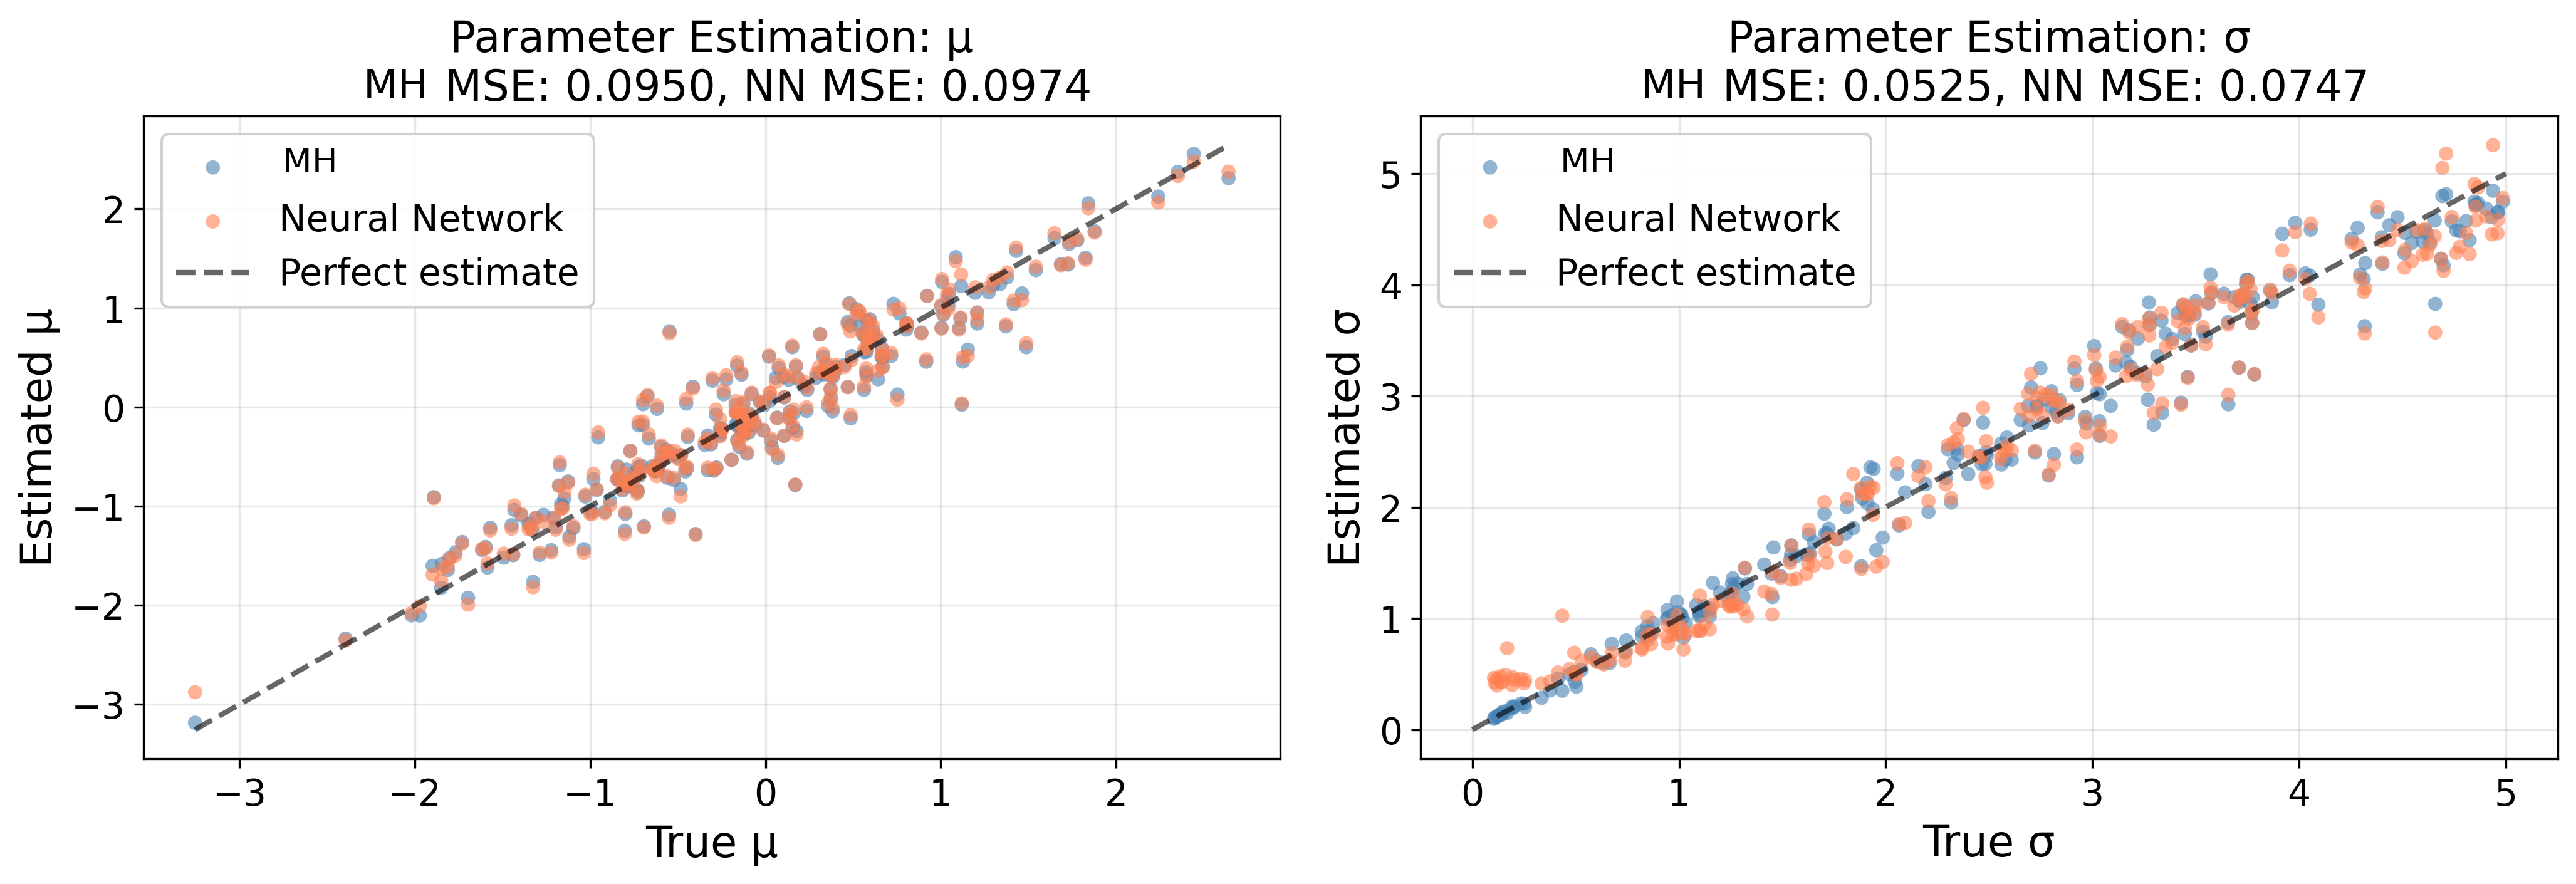
\includegraphics[width=\textwidth]{normal_model_estimates}
  \caption{Estimated against true parameter values for the normal
  model, across $256$ test datasets, for Metropolis--Hastings and
  the neural Bayes estimator. Both methods track the true parameters
  closely; the dashed line marks the hypothetical perfect estimation.}
  \label{fig:normal-model}
\end{figure}

\begin{table}[t]
  \centering
  \caption{Normal model: accuracy (mean squared error over the $256$
  test datasets) and per-dataset cost of the Metropolis--Hastings
  reference and the neural Bayes estimator. The two agree closely in
  accuracy, but the amortised network is faster per dataset by some
  three orders of magnitude (single-threaded CPU timing; $5{,}000$-step
  chains for Metropolis--Hastings).}
  \label{tab:normal-model}
  \begin{tabular}{l rr l}
    \toprule
    & $\mu$ (MSE) & $\sigma$ (MSE) & Cost per dataset \\
    \midrule
    Metropolis--Hastings   & $0.095$ & $0.053$ & $\approx 26$\,ms (re-run per dataset) \\
    Neural Bayes estimator & $0.097$ & $0.075$ & $\approx 9\,\mu$s (one forward pass) \\
    \bottomrule
  \end{tabular}
\end{table}

% ================================================================
%  CHAPTER 4 -- RAO-BLACKWELLISED LOSS FUNCTIONS  (CORE CHAPTER)
%  Experiment: tau-uniform sweep in final/sweeps2/ (+ floors_and_tables.py).
% ================================================================

\chapter{Rao-Blackwellised Loss Functions}
\label{ch:rao-blackwell}

Chapter~\ref{ch:amortization} established that training a neural Bayes
estimator is Monte Carlo integration of the Bayes risk, so the
training gradient is itself a Monte Carlo estimator with a variance.
This chapter reduces that variance by \emph{Rao-Blackwellisation}.
Rather than estimating the Bayes risk by sampling the whole parameter
vector, we integrate a conjugate block of it out of the loss
analytically and Monte Carlo approximate only what remains. Under
squared-error loss the construction is very simple: it
replaces the sampled target by its conditional posterior mean, and
the resulting training gradient is provably no noisier than the
standard one, for any model and any architecture. For the special case when the network is linear,
the guarantee strengthens further, from the gradient to the fitted
weights themselves.

The chapter has three sections.
Section~\ref{sec:rb-loss} develops the theory, Rao-Blackwellising the
loss function in general and then specialising to squared-error loss,
where the construction reduces to substituting a conditional posterior
mean and the training gradient it produces is provably no noisier than
the standard one.
Section~\ref{sec:rb-application} applies the method to Bayesian linear
regression, the simplest model with a non-trivial conjugate block.
Measured against a Gibbs-sampled Bayes-optimal reference, the
Rao-Blackwellised estimator attains a lower error than the standard
Monte Carlo estimator in every cell of a grid over parameter dimension
and batch size, closing about half of the gap to the Bayes-optimal
floor at the baseline, and matching the standard estimator at a quarter
of the minibatch size.
Section~\ref{sec:lr-discussion} discusses the result. This is the
unconditional improvement the theory predicts, and the central
empirical result of the thesis.


% ################################################################
% PART I -- THEORY
% ################################################################

% ----------------------------------------------------------------
\section{Rao-Blackwellising the loss function}
\label{sec:rb-loss}

% ----------------------------------------------------------------
\subsection{The Rao-Blackwell theorem}
\label{sec:rb-theorem}

The Rao-Blackwell theorem states that an estimator can always be
improved, under convex loss, by conditioning it on a sufficient
statistic~\citep{lehmann1998point}.

\begin{theorem}[Rao-Blackwell]
\label{thm:rao-blackwell}
Let $\hat{\bm{\theta}}(\mathbf{y})$ be an estimator of $\bm{\theta}$
under a loss $L(\bm{\theta}, \cdot)$ convex in its second argument and
with $\E_{\mathbf{y} \given \bm{\theta}}\big[L(\bm{\theta},
\hat{\bm{\theta}}(\mathbf{y}))\big] < \infty$, and let
$T = T(\mathbf{y})$ be a statistic sufficient for $\bm{\theta}$.
Define the conditioned estimator
%
\begin{equation}
  \hat{\bm{\theta}}_T(\mathbf{y})
  = \E\big[\hat{\bm{\theta}}(\mathbf{y}) \given T\big].
  \label{eq:rb-conditioned}
\end{equation}
%
Then $\hat{\bm{\theta}}_T$ is an estimator --- it does not depend on
the unknown $\bm{\theta}$ --- and its risk is no greater,
%
\begin{equation}
  R(\bm{\theta}, \hat{\bm{\theta}}_T)
  \;\le\;
  R(\bm{\theta}, \hat{\bm{\theta}})
  \qquad \text{for every } \bm{\theta}.
  \label{eq:rb-risk-inequality}
\end{equation}
\end{theorem}

\begin{proof}
Because $T$ is sufficient for $\bm{\theta}$, the conditional
distribution of $\mathbf{y}$ given $T$ does not depend on
$\bm{\theta}$; hence neither does the conditional expectation
defining $\hat{\bm{\theta}}_T$ in~\eqref{eq:rb-conditioned}, which is
therefore a genuine estimator rather than a function of the parameter
being estimated. Fix $\bm{\theta}$. Since $L(\bm{\theta}, \cdot)$ is
convex, the conditional form of Jensen's inequality gives, pointwise
in $T$,
%
\begin{equation}
  L\big(\bm{\theta}, \hat{\bm{\theta}}_T(\mathbf{y})\big)
  = L\big(\bm{\theta}, \E[\hat{\bm{\theta}}(\mathbf{y}) \given T]\big)
  \;\le\;
  \E\big[L(\bm{\theta}, \hat{\bm{\theta}}(\mathbf{y})) \given T\big].
\end{equation}
%
Take the expectation over $\mathbf{y} \given \bm{\theta}$ on both
sides; the tower property
$\E\big[\E[\,\cdot \given T]\big] = \E[\,\cdot\,]$ collapses the
right-hand side, giving
%
\begin{equation}
  R(\bm{\theta}, \hat{\bm{\theta}}_T)
  = \E\big[L(\bm{\theta}, \hat{\bm{\theta}}_T)\big]
  \le \E\big[\E[L(\bm{\theta}, \hat{\bm{\theta}}) \given T]\big]
  = \E\big[L(\bm{\theta}, \hat{\bm{\theta}})\big]
  = R(\bm{\theta}, \hat{\bm{\theta}}),
\end{equation}
%
which is~\eqref{eq:rb-risk-inequality}. When $L(\bm{\theta}, \cdot)$
is strictly convex the inequality is strict unless
$\hat{\bm{\theta}}(\mathbf{y})$ is already a function of $T$ alone, in
which case conditioning leaves it unchanged.
\end{proof}

The applications in this chapter use the theorem through the variance
it controls, and the mechanism is the \emph{law of total variance}: for
any random vector $Z$ and any conditioning variable $T$,
%
\begin{equation}
  \Var(Z)
  = \E\big[\Var(Z \given T)\big]
  + \Var\big(\E[Z \given T]\big),
  \label{eq:total-variance}
\end{equation}
%
and since $\E[\Var(Z \given T)] \succeq 0$ in the positive
semi-definite order,
%
\begin{equation}
  \Var\big(\E[Z \given T]\big) \;\preceq\; \Var(Z).
  \label{eq:rb-inequality}
\end{equation}
%
Replacing a random quantity by its conditional expectation cannot
increase its variance, for any conditioning variable, not
only a sufficient statistic, and strictly decreases it unless the
quantity is already a function of $T$. Every variance reduction below
is an instance of~\eqref{eq:rb-inequality}: in
Section~\ref{sec:gradients}, with $Z$ a Monte Carlo training gradient
and $T = (\mathbf{y}, \bm{\theta}_1)$; and in
Section~\ref{sec:linear-network}, with $Z$ the fitted weights.


% ----------------------------------------------------------------
\subsection{Rao-Blackwellising the Bayes risk}
\label{sec:rb-bayes-risk}

Let $\hat{\bm{\theta}}_{\bm{\gamma}}$ be a neural Bayes estimator with weights
$\bm{\gamma}$. By splitting the parameter vector into two blocks $\bm{\theta} =
(\bm{\theta}_1, \bm{\theta}_2)$, the Bayes risk can be written as:
%
\begin{equation}
  \begin{split}
    r(\bm{\gamma})
    &= \E_{\bm{\theta}, \mathbf{y}}
       \big[L(\bm{\theta},
       \hat{\bm{\theta}}_{\bm{\gamma}}(\mathbf{y}))\big] \\
    &= \int_{\Theta_1}\!\int_{\mathcal{Y}}\!\int_{\Theta_2}
       L(\bm{\theta},
       \hat{\bm{\theta}}_{\bm{\gamma}}(\mathbf{y}))\,
       p(\bm{\theta}_1, \mathbf{y}, \bm{\theta}_2)
       \dd\bm{\theta}_2 \dd\mathbf{y} \dd\bm{\theta}_1.
  \end{split}
  \label{eq:risk-integral}
\end{equation}
%
Factorising the joint density by the chain rule,
$p(\bm{\theta}_1, \mathbf{y}, \bm{\theta}_2) =
p(\bm{\theta}_2 \given \mathbf{y}, \bm{\theta}_1)\,
p(\mathbf{y} \given \bm{\theta}_1)\,p(\bm{\theta}_1)$, the
risk becomes a nested expectation,
%
\begin{equation}
  r(\bm{\gamma})
  = \E_{\bm{\theta}_1}\!\Big[
    \E_{\mathbf{y} \given \bm{\theta}_1}\!\big[
    \underbrace{\E_{\bm{\theta}_2 \given \mathbf{y}, \bm{\theta}_1}
    [L(\bm{\theta}, \hat{\bm{\theta}}_{\bm{\gamma}}(\mathbf{y}))]}
    _{=:\; f(\bm{\theta}_1, \mathbf{y})}\big]\Big].
  \label{eq:nested-risk}
\end{equation}
%
The inner expectation $f(\bm{\theta}_1, \mathbf{y})$ integrates
$\bm{\theta}_2$ out against its conditional posterior
$p(\bm{\theta}_2 \given \mathbf{y}, \bm{\theta}_1)$. The premise of
this chapter is that this inner integral is tractable, so that $f$ can
be evaluated in closed form, while the outer expectations over
$\bm{\theta}_1$ and $\mathbf{y}$ cannot, and must be estimated by
sampling.

The standard NBE training and the Rao-Blackwellised training differ in how much of~\eqref{eq:nested-risk}
they leave to that sampling. Both draw the same $K$ joint samples from
the model, each comprising parameters $\bm{\theta}_1^{(k)},
\bm{\theta}_2^{(k)}$ and the data $\mathbf{y}^{(k)}$ they generate.
The standard \emph{Monte Carlo} objective estimates the whole nested
expectation at once, feeding each sampled $\bm{\theta}_2^{(k)}$ into
the loss; the \emph{Rao-Blackwellised} objective uses
$\bm{\theta}_2^{(k)}$ only to simulate the data $\mathbf{y}^{(k)}$,
then discards it and evaluates the inner expectation $f$
analytically,
%
\begin{align}
  \hat{r}_{\MC}(\bm{\gamma})
  &= \frac{1}{K}\sum_{k=1}^{K}
     L\big(\bm{\theta}^{(k)},
     \hat{\bm{\theta}}_{\bm{\gamma}}(\mathbf{y}^{(k)})\big),
  \label{eq:rhat-mc} \\
  \hat{r}_{\RB}(\bm{\gamma})
  &= \frac{1}{K}\sum_{k=1}^{K}
     f\big(\bm{\theta}_1^{(k)}, \mathbf{y}^{(k)}\big),
  \label{eq:rhat-rb}
\end{align}
%
where $f(\bm{\theta}_1, \mathbf{y}) =
\E_{\bm{\theta}_2 \given \mathbf{y}, \bm{\theta}_1}
[L(\bm{\theta}, \hat{\bm{\theta}}_{\bm{\gamma}}(\mathbf{y}))]$ is the
inner integral of~\eqref{eq:nested-risk}, now evaluated in closed
form. The standard objective~\eqref{eq:rhat-mc} is exactly the
empirical Bayes risk of Chapter~\ref{ch:amortization}; the
Rao-Blackwellised
objective~\eqref{eq:rhat-rb} replaces each sampled loss term by its
conditional expectation given $(\bm{\theta}_1^{(k)},\mathbf{y}^{(k)})$, the draw $\bm{\theta}_2^{(k)}$ having served
only to generate the data. Both are unbiased estimators of the same
Bayes risk: taking the expectation of
either~\eqref{eq:rhat-mc} or~\eqref{eq:rhat-rb}
recovers~\eqref{eq:nested-risk}. The two objectives therefore share
the same minimiser, and differ only in variance.

When attempting to train the estimator by stochastic gradient descent, the variance of
the gradients we are using to train the estimator becomes important. Recall that the population gradient is the gradient of the Bayes risk, and so will be unchanged,
%
\begin{equation}
  g(\bm{\gamma}) = \nabla_{\bm{\gamma}} r(\bm{\gamma})
  = \nabla_{\bm{\gamma}} \E_{\bm{\theta}, \mathbf{y}}
    \big[ L(\bm{\theta}, \hat{\bm{\theta}}_{\bm{\gamma}}(\mathbf{y})) \big].
\end{equation}
%
The empirical training gradients $\hat{g}_{\MC}(\bm{\gamma})= \nabla_{\bm{\gamma}} \hat{r}_{\MC}(\bm{\gamma})$ and $\hat{g}_{\RB}(\bm{\gamma})= \nabla_{\bm{\gamma}} \hat{r}_{\RB}(\bm{\gamma})$, however, will differ between the two schemes, since they
are defined by the Monte Carlo estimates of the derivative of the Bayes risk with respect
to the neural network weights $\bm{\gamma}$.

% ----------------------------------------------------------------
\subsection{The squared-error case}
\label{sec:rb-mse}

Under squared-error loss $L(\bm{\theta}, \hat{\bm{\theta}}) = \|\bm{\theta} - \hat{\bm{\theta}}\|^2$, 
we can go further, and show the inner integral $f(\mathbf{y}, \bm{\theta}_1)$ always simplifies, regardless of the model.
If we write the estimator in block form
$\hat{\bm{\theta}}_{\bm{\gamma}}(\mathbf{y}) =
(\hat{\bm{\theta}}_{\bm{\gamma}}^{1}(\mathbf{y}),
\hat{\bm{\theta}}_{\bm{\gamma}}^{2}(\mathbf{y}))$ to match the partition of
$\bm{\theta}$, we can then separate the loss into components where only the
second term depends on $\bm{\theta}_2$.
%
\begin{align}
  f(\mathbf{y}, \bm{\theta}_1)
  &= \E_{\bm{\theta}_2 \given \mathbf{y}, \bm{\theta}_1}
     \big[\|\hat{\bm{\theta}}_{\bm{\gamma}}(\mathbf{y}) - \bm{\theta} \|^2\big]
   \notag \\[2pt]
   &= \E_{\bm{\theta}_2 \given \mathbf{y}, \bm{\theta}_1}
     \big[\ \|\hat{\bm{\theta}}_{\bm{\gamma}}^{1} - \bm{\theta}_1\|^2 + \|\hat{\bm{\theta}}_{\bm{\gamma}}^{2} - \bm{\theta}_2\|^2\big]
   \notag \\[2pt]
  &= \|\hat{\bm{\theta}}_{\bm{\gamma}}^{1} - \bm{\theta}_1\|^2
   + \E_{\bm{\theta}_2 \given \mathbf{y}, \bm{\theta}_1}
     \big[\|\hat{\bm{\theta}}_{\bm{\gamma}}^{2} - \bm{\theta}_2\|^2\big]
   \notag \\[2pt]
  &= \|\hat{\bm{\theta}}_{\bm{\gamma}}^{1} - \bm{\theta}_1\|^2
   + \big\|\hat{\bm{\theta}}_{\bm{\gamma}}^{2} - \E[\bm{\theta}_2 \given \mathbf{y}, \bm{\theta}_1]\big\|^2
   + \Tr\!\big(\Var(\bm{\theta}_2 \given \mathbf{y}, \bm{\theta}_1)
     \big),
  \label{eq:rb-mse}
\end{align}
%
where the final line applies the identity
$\E[\|Z - c\|^2] = \|\E[Z] - c\|^2 + \Tr(\Var(Z))$ to the random
vector $\bm{\theta}_2$ and the constant
$\hat{\bm{\theta}}_{\bm{\gamma}}^{2}$.

Two features of~\eqref{eq:rb-mse} drive everything that follows.
First, the sampled target $\bm{\theta}_2$ has been replaced by the
\emph{conditional posterior mean}
$\E[\bm{\theta}_2 \given \mathbf{y}, \bm{\theta}_1]$:
Rao-Blackwellising a squared-error loss simply substitutes the
conditional mean for the sampled value. Second, the trace term
$\Tr(\Var(\bm{\theta}_2 \given \mathbf{y}, \bm{\theta}_1))$ does not
depend on the weights $\bm{\gamma}$. It contributes nothing to the
gradient and need not be computed during training; it shifts the loss
by a constant but leaves the optimisation unchanged.

In practice, what has been done is that the training pairs $(\mathbf{y}, \bm{\theta})$ have been replaced with pairs $(\mathbf{y}, \bm{\theta}^{\mathrm{RB}})$, where $\bm{\theta}^{\mathrm{RB}}$ has the same posterior mean but less variance than $\bm{\theta}$. Intuitively, this should improve training of the neural network. In the limit, if one had the posterior mean of $\bm{\theta}$ already available, the network could be trained on $(\mathbf{y}, \E[\bm{\theta} \given \mathbf{y}])$ pairs. Of course, in this case, one would generally expect the neural network to be unnecessary except perhaps as a faster surrogate replacing direct analytical calculation of the posterior mean.

% ----------------------------------------------------------------
\subsection{The training gradients}
\label{sec:gradients}

Training minimises the objective by stochastic gradient descent
where each step moves the weights along
an estimate of the gradient of the objective with respect to
$\bm{\gamma}$. The objects to compare between the two schemes are
therefore not the objectives themselves but their gradients, and this
section derives them.

Both follow from differentiating their respective squared-error loss,
%
\begin{align}
  r_{\MC}(\bm{\gamma})
  &= \E_{\bm{\theta}}\Big[ \E_{\mathbf{y} \given \bm{\theta}}\big[
     \|\hat{\bm{\theta}}_{\bm{\gamma}}^{1}(\mathbf{y}) - \bm{\theta}_1\|^2
     + \|\hat{\bm{\theta}}_{\bm{\gamma}}^{2}(\mathbf{y}) - \bm{\theta}_2\|^2
     \big]\Big], \\
  r_{\RB}(\bm{\gamma})
  &= \E_{\bm{\theta}_1}\Big[ \E_{\mathbf{y} \given \bm{\theta}_1}\big[
     \|\hat{\bm{\theta}}_{\bm{\gamma}}^{1}(\mathbf{y}) - \bm{\theta}_1\|^2
     + \|\hat{\bm{\theta}}_{\bm{\gamma}}^{2}(\mathbf{y})
       - \E[\bm{\theta}_2 \given \mathbf{y}, \bm{\theta}_1]\|^2
     + \Tr\!\big(\Var(\bm{\theta}_2 \given \mathbf{y}, \bm{\theta}_1)\big)
     \big]\Big].
\end{align}
%
By differentiating each with respect to the weights $\bm{\gamma}$, we obtain the gradients for the two schemes:
%
\begin{align}
  g_{\MC}(\bm{\gamma})
  &= 2\,\E_{\bm{\theta}, \mathbf{y}}\big[
     (\nabla_{\bm{\gamma}} \hat{\bm{\theta}}_{\bm{\gamma}}^{1}(\mathbf{y}))^{\!\top}
     (\hat{\bm{\theta}}_{\bm{\gamma}}^{1}(\mathbf{y}) - \bm{\theta}_1) \big]
   + 2\,\E_{\bm{\theta}, \mathbf{y}}\big[
     (\nabla_{\bm{\gamma}} \hat{\bm{\theta}}_{\bm{\gamma}}^{2}(\mathbf{y}))^{\!\top}
     (\hat{\bm{\theta}}_{\bm{\gamma}}^{2}(\mathbf{y}) - \bm{\theta}_2) \big], \\
  g_{\RB}(\bm{\gamma})
  &= 2\,\E_{\bm{\theta}_1, \mathbf{y}}\big[
     (\nabla_{\bm{\gamma}} \hat{\bm{\theta}}_{\bm{\gamma}}^{1}(\mathbf{y}))^{\!\top}
     (\hat{\bm{\theta}}_{\bm{\gamma}}^{1}(\mathbf{y}) - \bm{\theta}_1) \big]
   + 2\,\E_{\bm{\theta}_1, \mathbf{y}}\big[
     (\nabla_{\bm{\gamma}} \hat{\bm{\theta}}_{\bm{\gamma}}^{2}(\mathbf{y}))^{\!\top}
     (\hat{\bm{\theta}}_{\bm{\gamma}}^{2}(\mathbf{y})
       - \E[\bm{\theta}_2 \given \mathbf{y}, \bm{\theta}_1]) \big].
\end{align}
%
To show that $g_{\RB}(\bm{\gamma})$ is less noisy than $g_{\MC}(\bm{\gamma})$, we examine the variance of the stochastic components inside the expectations. Specifically, we look at the second term of each gradient:
%
\begin{align}
  G_{\MC}^{(2)} &= 2\,J_{\bm{\gamma}}(\mathbf{y})^{\!\top}(\hat{\bm{\theta}}_{\bm{\gamma}}^{2}(\mathbf{y}) - \bm{\theta}_2),  \\
  G_{\RB}^{(2)} &= 2\,J_{\bm{\gamma}}(\mathbf{y})^{\!\top}(\hat{\bm{\theta}}_{\bm{\gamma}}^{2}(\mathbf{y})
     - \E[\bm{\theta}_2 \given \mathbf{y}, \bm{\theta}_1]), \qquad \text{where} \quad J_{\bm{\gamma}}(\mathbf{y}) \equiv \nabla_{\bm{\gamma}} \hat{\bm{\theta}}_{\bm{\gamma}}^{2}(\mathbf{y}).
\end{align}
%
Note here that $G^{(2)}_{\RB}=\E[G_{\MC}^{(2)} \given \mathbf{y}, \bm{\theta}_{1}]$:
conditional on $(\mathbf{y}, \bm{\theta}_1)$ the estimate
$\hat{\bm{\theta}}_{\bm{\gamma}}^{2}(\mathbf{y})$ and its Jacobian are fixed, and
the sampled $\bm{\theta}_2$ enters $G_{\MC}^{(2)}$ linearly, so conditioning
simply replaces $\bm{\theta}_2$ by its conditional mean. The Rao-Blackwellised
gradient term is thus the conditional expectation of the Monte Carlo one, and
by the tower property the two share the same mean,
$\E[G_{\RB}^{(2)}] = \E[G_{\MC}^{(2)}]$, so the substitution introduces no bias;
and the law of total variance~\eqref{eq:total-variance} gives a gap that is an
average of conditional covariances,
%
\begin{equation}
  \Var\big(G_{\MC}^{(2)}\big) - \Var\big(G_{\RB}^{(2)}\big)
  = \E\big[\Var\big(G_{\MC}^{(2)} \given \mathbf{y}, \bm{\theta}_1\big)\big]
  \;\succeq\; 0.
  \label{eq:variance-gap}
\end{equation}
%
This gap concerns only the second term. The first is unaffected:
\[
  G^{(1)} = 2\,(\nabla_{\bm{\gamma}} \hat{\bm{\theta}}_{\bm{\gamma}}^{1}(\mathbf{y}))^{\!\top}
  (\hat{\bm{\theta}}_{\bm{\gamma}}^{1}(\mathbf{y}) - \bm{\theta}_1)
\]
is already a function of $(\mathbf{y}, \bm{\theta}_1)$, so
$\E[G^{(1)} \given \mathbf{y}, \bm{\theta}_1] = G^{(1)}$. Combined with
$G^{(2)}_{\RB} = \E[G^{(2)}_{\MC} \given \mathbf{y}, \bm{\theta}_1]$, the entire
per-sample gradient is the conditional expectation of the standard one, and
averaging over the minibatch preserves this, so
$\hat{g}_{\RB} = \E[\hat{g}_{\MC} \given \mathbf{y}, \bm{\theta}_1]$. The law of
total variance~\eqref{eq:total-variance} therefore applies to the whole gradient
vector, not merely its second term:
%
\begin{equation}
  \Var(\hat{g}_{\MC}) - \Var(\hat{g}_{\RB})
  = \E\big[\Var(\hat{g}_{\MC} \given \mathbf{y}, \bm{\theta}_1)\big]
  \;\succeq\; 0.
  \label{eq:full-variance-gap}
\end{equation}
%
This is positive semi-definite. Rao-Blackwellisation can therefore never
increase the variance of the training gradient, and, since nothing in the
argument used any property of the network, the guarantee holds for every
model and every architecture.

To quantify this \emph{variance gap}, we can substitute $G_{\MC}^{(2)}$ into \eqref{eq:variance-gap} and apply the identity $\Var(AZ) = A \Var(Z) A^{\!\top}$ for random vector $Z$ and constant matrix $A$.
%
\begin{equation}
\Var\!\left( G_{\MC}^{(2)} \given \mathbf y,\bm{\theta}_1 \right) = 4\, J_{\bm{\gamma}}^{\!\top} \Var(\bm{\theta}_2\given \mathbf y,\bm{\theta}_1) J_{\bm{\gamma}},
\label{eq:general-gradient-cov-gap}
\end{equation}
%
This shows the reduction scales with two interpretable quantities. The first is the conditional posterior covariance $\Var(\bm{\theta}_2\given \mathbf y,\bm{\theta}_1)$, which is large exactly when $\bm{\theta}_2$ is weakly identified by the data --- the case where the sampled target is noisiest and stands to gain the most from being replaced. The second is the Jacobian $J_{\bm{\gamma}}$, which is generally largest early in training, when the network weights are far from optimal. Taken together, these suggest that the variance reduction is greatest precisely when the optimiser most needs a clean signal: early in training, and on weakly identified parameters.





% ----------------------------------------------------------------
\subsection{The linear network case}
\label{sec:linear-network}

Rao-Blackwellisation reduces the variance of the training gradient;
it is natural to ask what this implies for the estimator that
training produces. For a \emph{linear network}, one whose output is
linear in its weights, the question can be answered exactly.

A linear network passes the data through a fixed feature map
$z(\mathbf{y})$ and reads the estimate off as a linear combination of
the resulting features,
%
\begin{equation}
  \hat{\bm{\theta}}_{\bm{\gamma}}(\mathbf{y})
  = z(\mathbf{y})^{\!\top} \bm{\gamma},
  \label{eq:linear-net}
\end{equation}
%
with weight vector $\bm{\gamma}$. Because the feature map is fixed,
the estimate is linear in $\bm{\gamma}$.

Consider $K$ simulated datasets, dataset $k$ carrying the estimand
$\bm{\theta}^{(k)}$ and data $\mathbf{y}^{(k)}$. Collect the estimands
into the rows of a matrix $\Theta$ and the feature vectors
$z(\mathbf{y}^{(k)})$ into the rows of a matrix $Z$. Fitting the
linear network~\eqref{eq:linear-net} by least squares over the $K$
datasets gives the weight vector
%
\begin{equation}
  \hat{\bm{\gamma}}
  = (Z^{\!\top} Z)^{-1} Z^{\!\top}\, \Theta.
  \label{eq:ols}
\end{equation}
%
Both training schemes fit on the same $K$ datasets, so they share the
feature matrix $Z$ and hence the matrix
$A := (Z^{\!\top}Z)^{-1}Z^{\!\top}$ of~\eqref{eq:ols}; the schemes
differ only in the estimand matrix $\Theta$. Standard training stacks
the sampled estimands into $\Theta_{\MC}$; Rao-Blackwellised training
stacks the same rows with each $\bm{\theta}_2$-block replaced by its
conditional posterior mean. Writing
$T = \{(\mathbf{y}^{(k)}, \bm{\theta}_1^{(k)})\}_{k=1}^{K}$ for the
data and the $\bm{\theta}_1$-blocks of every dataset, and using the fact
the datasets are simulated independently, the two estimand matrices
are related, row by row, by a single conditional expectation,
%
\begin{equation}
  \Theta_{\RB} = \E[\Theta_{\MC} \given T].
  \label{eq:theta-rb}
\end{equation}
%
Column $j$ of the weight matrix is $\hat{\bm{\gamma}}_{(j)} =
A\,\Theta_{(j)}$. Because $A$ is built from the data alone it is fixed
given $T$; combining this with~\eqref{eq:theta-rb}, the constant
matrix passes straight through the conditional expectation,
%
\begin{equation}
  \hat{\bm{\gamma}}_{(j)}^{\RB}
  = A\,\Theta_{(j)}^{\RB}
  = A\,\E\big[\Theta_{(j)}^{\MC} \given T\big]
  = \E\big[A\,\Theta_{(j)}^{\MC} \given T\big]
  = \E\big[\hat{\bm{\gamma}}_{(j)}^{\MC} \given T\big].
  \label{eq:gamma-rb}
\end{equation}
%
The fitted Rao-Blackwellised weights are therefore the
Rao-Blackwellisation of the fitted standard weights, with $T$ the
conditioning variable. The law of total variance~\eqref{eq:rb-inequality}
applies again,
%
\begin{equation}
  \Var\big(\hat{\bm{\gamma}}_{(j)}^{\MC}\big)
  - \Var\big(\hat{\bm{\gamma}}_{(j)}^{\RB}\big)
  = \E\big[\Var(\hat{\bm{\gamma}}_{(j)}^{\MC} \given T)\big]
  \;\succeq\; 0.
  \label{eq:linear-result}
\end{equation}
%
For a linear network, then, Rao-Blackwellisation not only reduces the variance of the training gradient; it reduces the variance
of the fitted weights themselves, for any finite training set.
The Rao-Blackwellised estimator makes more efficient use of the same
simulated data.

A fully nonlinear network does not admit the closed
 form~\eqref{eq:ols}, and no such exact statement is available in general. However, the
linear result is suggestive of the nonlinear case: if
every layer but the last is held fixed, training the final layer is
exactly the linear problem above, with $z$ the feature map computed
by the fixed layers, so the
argument~\eqref{eq:linear-net}--\eqref{eq:linear-result} applies to
the final layer (with linear activation) of any network, be it linear or nonlinear. A complete treatment of the nonlinear
case is left to future work.


% ################################################################
% PART II -- EXPERIMENT: BAYESIAN LINEAR REGRESSION
% ################################################################

% ----------------------------------------------------------------
\section{Application to Bayesian linear regression}
\label{sec:rb-application}

% ----------------------------------------------------------------
\subsection{The Bayesian linear regression model}
\label{sec:lr-model}

We tested the method on Bayesian linear regression, Example~2 from Section~\ref{sec:cs-linreg}. The
model~\eqref{eq:lr-model} is
$\bm{\beta} \sim \Normal(\mathbf{0}, \sigma_0^2 I_p)$,
$\tau \sim \Uniform(\tau_{\text{low}}, \tau_{\text{high}})$, and
$\mathbf{y} \given \bm{\beta}, \tau \sim
\Normal(X\bm{\beta}, \tau^{-1} I_{n})$ for a fixed design matrix
$X \in \reals^{n \times p}$. This model is an ideal test case for Rao-Blackwellisation because it is simple and well-understood. The estimand is $\bm{\theta} = (\bm{\beta}^{\!\top}, \sigma)^{\!\top}$,
of dimension $p+1$. In the notation of Section~\ref{sec:rb-loss},
$\bm{\theta}_2 = \bm{\beta}$ is the conjugate block to be integrated
out and $\bm{\theta}_1 = \sigma$ is the sampled block.

The model is conditionally conjugate in both blocks, as
Section~\ref{sec:conj-linreg} derives. Two of those conditionals matter
here. Given the precision, the coefficients have the Gaussian
conditional
$\bm{\beta} \given \mathbf{y}, \tau \sim
\Normal(\bm{\beta}_n, \Sigma_n)$ of~\eqref{eq:lr-conditional}, with
covariance and mean
$\Sigma_n = (\sigma_0^{-2} I_p + \tau X^{\!\top}X)^{-1}$ and
$\bm{\beta}_n = \Sigma_n\,\tau X^{\!\top}\mathbf{y}$
of~\eqref{eq:lr-defs}; given the coefficients, the precision has the
truncated-Gamma conditional~\eqref{eq:lr-tau-posterior}. The Gaussian
$\bm{\beta}$-conditional is the structure that the Rao-Blackwellised
loss of Section~\ref{sec:lr-losses} exploits, and both conditionals
drive the Gibbs sampler used for the Bayes floor in
Section~\ref{sec:bayes-floor}.

% ----------------------------------------------------------------
\subsection{Monte Carlo and Rao-Blackwellised training losses}
\label{sec:lr-losses}

The standard (Monte Carlo) per-sample loss is the squared error
against the sampled parameters,
%
\begin{equation}
  \ell_{\MC}(\bm{\gamma})
  = \|\hat{\bm{\theta}}_{\bm{\gamma}}^{\beta}(\mathbf{y}) - \bm{\beta}\|^2
  + (\hat{\bm{\theta}}_{\bm{\gamma}}^{\sigma}(\mathbf{y}) - \sigma)^2.
  \label{eq:lr-mc-loss}
\end{equation}
%
Applying the squared-error construction of
Section~\ref{sec:rb-mse} with the conjugate
posterior~\eqref{eq:lr-conditional} gives the Rao-Blackwellised loss
%
\begin{equation}
  \ell_{\RB}(\bm{\gamma})
  = \|\hat{\bm{\theta}}_{\bm{\gamma}}^{\beta}(\mathbf{y})
      - \bm{\beta}_n(\sigma, \mathbf{y})\|^2
  + \Tr(\Sigma_n)
  + (\hat{\bm{\theta}}_{\bm{\gamma}}^{\sigma}(\mathbf{y}) - \sigma)^2,
  \label{eq:lr-rb-loss}
\end{equation}
%
in which the sampled $\bm{\beta}$ is replaced by the conditional mean
$\bm{\beta}_n$ and the trace term $\Tr(\Sigma_n)$, being independent
of $\bm{\gamma}$, contributes no gradient. The two losses have the
same population minimiser; they differ only in the variance of the
stochastic gradient, exactly as Section~\ref{sec:rb-loss} describes.

% ----------------------------------------------------------------
\subsection{Quantifying the variance reduction}
\label{sec:lr-variance-reduction}

The trace term in~\eqref{eq:lr-rb-loss} is constant in the network
weights, so it does not enter the optimisation. It is nevertheless
the quantity that explains when Rao-Blackwellisation should be most
effective. Conditional on $(\mathbf{y},\tau)$, the sampled coefficient
target decomposes as
%
\begin{equation}
  \bm{\beta}
  =
  \bm{\beta}_n
  +
  \bm{\varepsilon},
  \qquad
  \bm{\varepsilon} \given \mathbf{y},\tau
  \sim
  \Normal(\mathbf{0},\Sigma_n).
\end{equation}
%
Thus the Monte Carlo target differs from the Rao-Blackwellised target
by a zero-mean posterior fluctuation with covariance $\Sigma_n$. For
any beta-head prediction
$\hat{\bm{\theta}}_{\bm{\gamma}}^\beta(\mathbf{y})$, the conditional
squared-error risk satisfies
%
\begin{equation}
  \E\!\left[
  \|\hat{\bm{\theta}}_{\bm{\gamma}}^\beta(\mathbf{y})-\bm{\beta}\|^2
  \given \mathbf{y},\tau
  \right]
  =
  \|\hat{\bm{\theta}}_{\bm{\gamma}}^\beta(\mathbf{y})-\bm{\beta}_n\|^2
  +
  \Tr(\Sigma_n).
  \label{eq:lr-target-noise}
\end{equation}
%
The term $\Tr(\Sigma_n)$ is therefore the conditional target variance
seen by the Monte Carlo loss and removed by the Rao-Blackwellised loss.

The same quantity controls the gradient noise. Let
$J_{\bm{\gamma}}(\mathbf{y}) =
\nabla_{\bm{\gamma}}\hat{\bm{\theta}}_{\bm{\gamma}}^\beta(\mathbf{y})$
denote the Jacobian of the beta-head with respect to the network
weights. The beta part of the Monte Carlo gradient is
%
\begin{equation}
  G_{\MC}^{\beta}
  =
  2J_{\bm{\gamma}}(\mathbf{y})^{\!\top}
  \left(
  \hat{\bm{\theta}}_{\bm{\gamma}}^\beta(\mathbf{y})-\bm{\beta}
  \right),
\end{equation}
%
while the Rao-Blackwellised gradient replaces $\bm{\beta}$ by
$\bm{\beta}_n$. Conditional on $(\mathbf{y},\tau)$, the latter is
fixed and the only remaining randomness in $G_{\MC}^{\beta}$ is the
posterior fluctuation $\bm{\beta}-\bm{\beta}_n$. Hence
%
\begin{equation}
  \Var\!\left(
  G_{\MC}^{\beta}
  \given \mathbf{y},\tau
  \right)
  =
  4J_{\bm{\gamma}}(\mathbf{y})^{\!\top}
  \Sigma_n
  J_{\bm{\gamma}}(\mathbf{y}),
  \label{eq:lr-gradient-cov-gap}
\end{equation}
%
which is precisely the conditional gradient variance removed by
Rao-Blackwellisation.

The size of this removed component can be read directly from the
spectrum of the design matrix. If
$\lambda_1,\ldots,\lambda_p$ are the eigenvalues of $X^{\!\top}X$, then
%
\begin{equation}
  \Tr(\Sigma_n)
  =
  \sum_{j=1}^{p}
  \frac{1}{\sigma_0^{-2}+\tau\lambda_j}
  =
  \sigma_0^2
  \sum_{j=1}^{p}
  \frac{1}{1+\tau\sigma_0^2\lambda_j}.
  \label{eq:lr-trace-spectrum}
\end{equation}
%
Each summand corresponds to one coefficient direction. Directions with
large $\lambda_j$ are well identified by the data and contribute
little posterior variance; directions with small $\lambda_j$ remain
uncertain and contribute close to the prior variance $\sigma_0^2$.
Thus Rao-Blackwellisation should be most effective in regimes where
many coefficient directions are weakly identified: high-dimensional
problems, ill-conditioned designs, noisy observations, or small
sample sizes.

Under the uniform precision prior used in the experiment,
$\tau\sim\Uniform(\tau_{\mathrm{low}},\tau_{\mathrm{high}})$, the
expected removed target variance has the closed form
%
\begin{equation}
  \E_{\tau}\!\left[\Tr(\Sigma_n)\right]
  =
  \frac{1}{\tau_{\mathrm{high}}-\tau_{\mathrm{low}}}
  \sum_{j=1}^{p}
  \frac{
  \log(\sigma_0^{-2}+\tau_{\mathrm{high}}\lambda_j)
  -
  \log(\sigma_0^{-2}+\tau_{\mathrm{low}}\lambda_j)
  }{\lambda_j},
  \label{eq:lr-expected-trace}
\end{equation}
%

% ----------------------------------------------------------------
\subsection{The Gibbs benchmark}
\label{sec:bayes-floor}

To provide us with a reference for both neural networks' training performance,
 the natural yardstick is the lowest loss that any
estimator can attain, the \emph{Bayes-optimal floor},
%
\begin{align}
  L^{*}
  &= \E_{\mathbf{y}}\!\Big[
     \E_{\bm{\theta} \given \mathbf{y}}
     \big[\|\bm{\theta}
     - \E[\bm{\theta} \given \mathbf{y}]\|^2\big]\Big]
   \notag\\[2pt]
  &= \E_{\mathbf{y}}\!\big[\Tr\Var(\bm{\theta} \given \mathbf{y})\big],
  \label{eq:floor-def}
\end{align}
%
attained by the posterior mean, so the floor is
the expected posterior variance: the irreducible uncertainty that
remains once the data have been seen. A network whose loss reaches
$L^{*}$ is doing as well as any estimator could.

The floor cannot be evaluated directly: neither the posterior mean
nor the posterior variance in~\eqref{eq:floor-def} is available in
closed form, because the joint posterior
$p(\bm{\beta}, \tau \given \mathbf{y})$ is not a standard
distribution. Its two conditionals are, however, standard
(Section~\ref{sec:conj-linreg}), so it can be sampled by the Gibbs
sampler of Example~2 (Section~\ref{sec:cs-linreg}): each sweep draws
$\bm{\beta}$ from the
Gaussian conditional~\eqref{eq:lr-conditional} through the Cholesky
factor of $\Sigma_n^{-1}$, and $\tau$ from the truncated-Gamma
conditional~\eqref{eq:lr-tau-posterior} by inverse-CDF sampling.

\paragraph{Gibbs as a benchmark.}
The sampler is run on a held-out test set of problems. After a
burn-in of discarded sweeps, the retained draws
$\{(\bm{\beta}^{(s)}, \tau^{(s)})\}_{s=1}^{S}$ are post-processed: the
noise scale of each draw is recovered as
$\sigma^{(s)} = (\tau^{(s)})^{-1/2}$ before averaging. The chain average then converges to the posterior mean as
$S \to \infty$.
\begin{align}
  \tfrac{1}{S}\sum_s (\bm{\beta}^{(s)}, \sigma^{(s)}) \longrightarrow \E[\bm{\theta} \given \mathbf{y}]
\end{align}

With the posterior mean in hand for each test problem, the benchmark
$L^{*}$ is estimated as the mean squared error of that estimate
against the true $\bm{\theta}$, averaged over the test set. It is
therefore computed in exactly the way the test loss of the neural
estimators is, so the comparison of Section~\ref{sec:lr-results} is
like-for-like.

% ----------------------------------------------------------------
\subsection{Experimental design}
\label{sec:lr-design}

We train both the standard Monte Carlo estimator and the Rao-Blackwellised estimator
on simulated datasets from the Bayesian linear regression model.

For each value of $p$, a single design matrix $X \in \mathbb{R}^{n \times p}$ is drawn once 
and then fixed across all training and testing simulations. Its entries are sampled independently 
from a standard normal distribution and the columns are standardised to have comparable 
scale. This ensures that differences between Monte Carlo and Rao-Blackwellised training are 
not confounded by changing the regression design across runs.

The estimator is a three-layer multilayer perceptron of hidden width
$128$ with ReLU activations and a softplus output on the $\sigma$-head
to enforce positivity, trained with Adam~\citep{kingma2015adam} at
learning rate $10^{-3}$. The two schemes are trained from identical
initialisations on the same simulated batches, so that any difference
between them is attributable to the loss alone. The experiment sweeps
the parameter dimension $p \in \{2, 5, 10, 20, 30\}$ and the minibatch
size $\{4, 16, 64, 256\}$ at a fixed sample size $n = 50$, training
each cell for $200$ epochs over ten seeds. The precision prior is
$\tau = \sigma^{-2} \sim \Uniform(0.01, 1)$, placing the noise scale in
$\sigma \in (1, 10)$.

A single design matrix $X$ is fixed per dimension. Because the
population loss depends on $X$, each panel of
Figure~\ref{fig:curves} corresponds to one inference task and results
are aggregated only over training seeds, never pooled across design
matrices. The Bayes-optimal floor $L^{*}$ for each dimension is
computed by the Gibbs sampler of Section~\ref{sec:bayes-floor} on a
held-out test set, in exactly the way the test loss of the neural
estimators is, so the comparison of Section~\ref{sec:lr-results} is
like-for-like.

% ----------------------------------------------------------------
\subsection{Results}
\label{sec:lr-results}

\paragraph{Rao-Blackwellisation beats Monte Carlo in every cell.}
\label{sec:lr-main-grid}
Figure~\ref{fig:curves} shows the training curves of the two
estimators across the grid of parameter dimension $p$ and batch size,
at the baseline sample size $n = 50$, as the seed mean with a
$\pm 1$ standard-deviation band. The Rao-Blackwellised runs sit below
the Monte Carlo runs in every panel, and the separation persists
across all four batch sizes: a larger batch lowers both methods
but does not close the gap between them.

\begin{figure}[H]
  \centering
  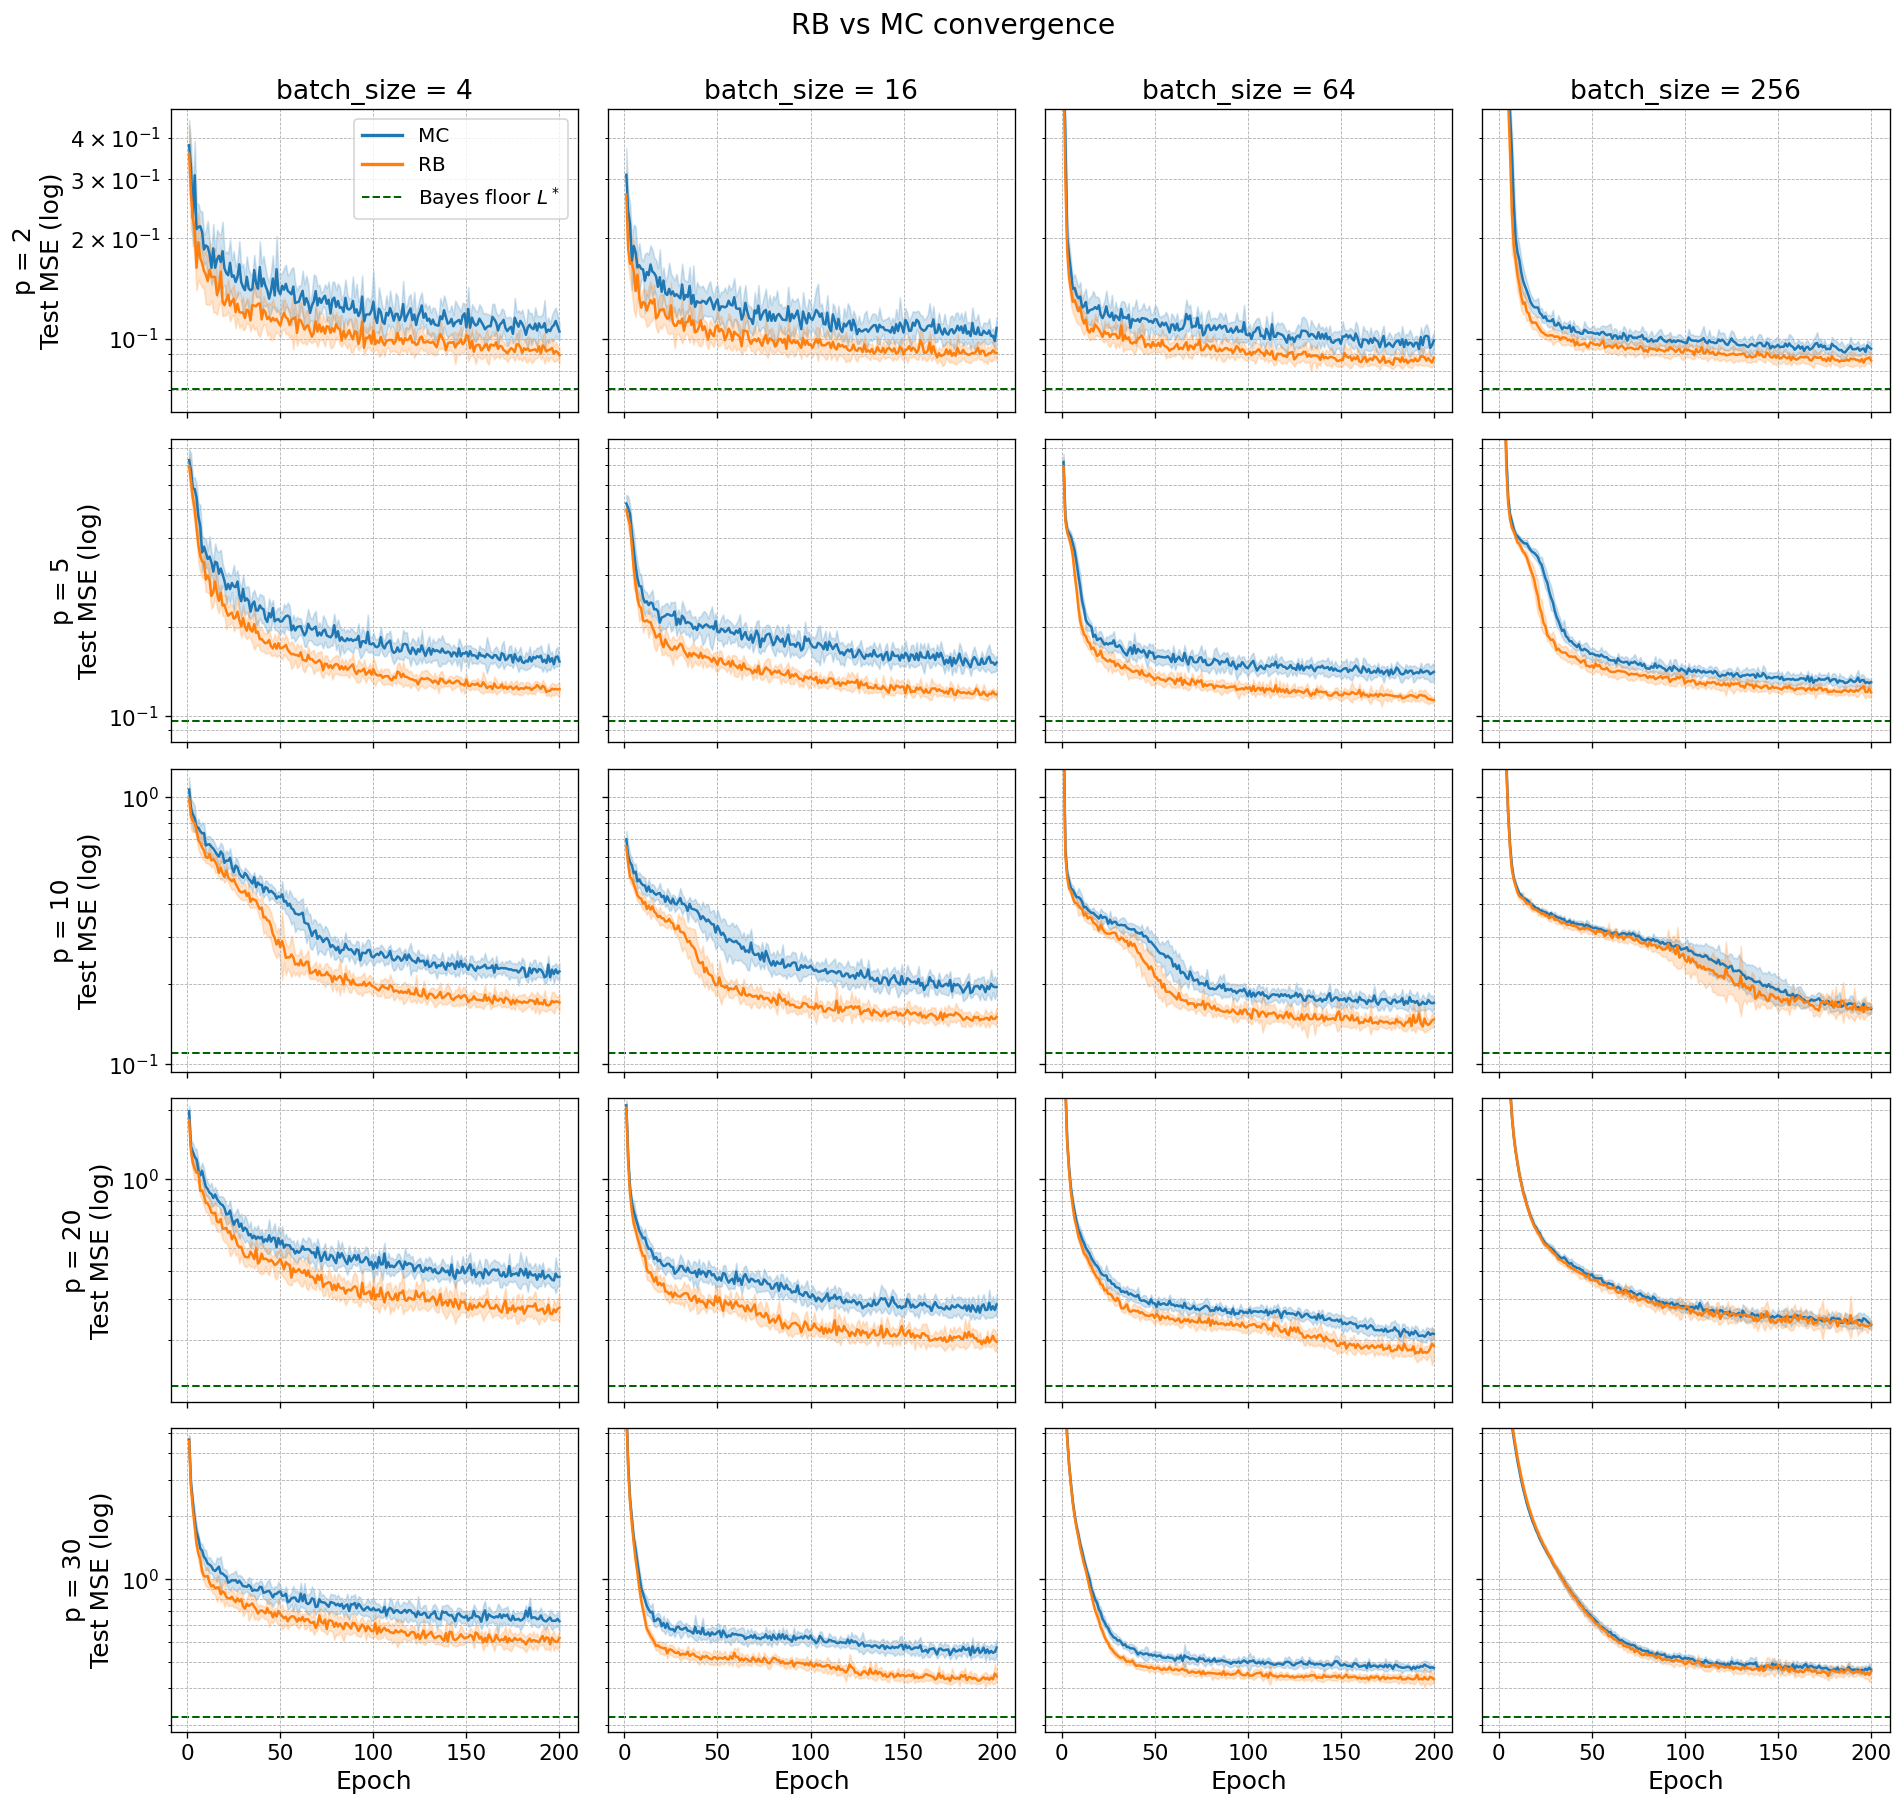
\includegraphics[width=\textwidth]{rb_tau_curves}
  \caption{Training curves across parameter dimension
  $p \in \{2, 5, 10, 20, 30\}$ (rows) and batch size
  $\{4, 16, 64, 256\}$ (columns), at sample size $n = 50$ under the
  precision prior $\tau = \sigma^{-2} \sim \Uniform(0.01, 1)$
  (equivalently $\sigma \in (1, 10)$). Each panel shows the mean over
  seeds with a $\pm 1$ standard-deviation band --- Monte Carlo (MC) in
  blue, Rao-Blackwellised (RB) in orange. The dark green dashed line in
  each panel marks the Bayes-optimal floor $L^{*}(p)$ for that dimension. RB
  tracks at or below MC in every panel, at every batch size, and nearer
  the floor.}
  \label{fig:curves}
\end{figure}

This pattern holds across the whole grid: the Rao-Blackwellised
estimator attains a lower final loss than the Monte Carlo estimator in
all twenty $(p, \text{batch})$ cells (Appendix~\ref{app:main-grid}), and
the advantage persists on a second, independent design matrix
(Appendix~\ref{app:second-design}).
This is consistent with the covariance calculation of
Section~\ref{sec:lr-variance-reduction}. Increasing the parameter
dimension adds coefficient directions to the sum
\eqref{eq:lr-trace-spectrum}; when these directions are weakly
identified, they contribute additional posterior target variance to
the Monte Carlo gradient. Increasing the batch size has the opposite
effect on the observed gap: it does not change $\Tr(\Sigma_n)$ for an
individual simulated problem, but it averages that target noise over
more simulations, giving a $1/B$ scaling.


\paragraph{Approaching the Bayes floor.}
\label{sec:lr-asymptotic}
We can compare the neural estimators to the Bayes-optimal floor. At the
baseline cell ($p = 20$, batch $16$) the Monte Carlo estimator reaches
a final loss of $0.276$ and the Rao-Blackwellised estimator $0.198$,
against a floor of $L^{*} = 0.126$: the Rao-Blackwellised estimator
closes about half (some $52\%$) of the gap between the Monte Carlo
loss and the unreachable floor. The size of the gain varies across the
grid with the excess-over-floor ratio
$(\mathcal{L}_{\MC} - L^{*})/(\mathcal{L}_{\RB} - L^{*})$, which runs
from near one at the largest batch, where both estimators have nearly
exhausted the Monte Carlo noise, to above two at the smaller batches
(Appendix~\ref{app:main-grid}).

In some of the training curves, we observe both training curves coming asymptotically to different levels. Although, RB and MC have the same population asymptote, under finite-batch fixed-step optimisation they can have different effective asymptotes; RB's is lower because it removes a positive semi-definite component of the gradient covariance. This phenomenon could be minimised by applying a \emph{learning rate scheduler}, a standard neural network technique which dynamically adjusts the learning rate as training progresses.

\paragraph{Rao-Blackwellisation versus larger batches.}
\label{sec:lr-batch}
Both Rao-Blackwellisation and a larger minibatch reduce the noise in
the training gradient (the former by removing the sampled-coefficient
variance analytically, the latter by averaging it over more samples),
so it is natural to ask whether Rao-Blackwellisation is simply a larger
batch in disguise. A batch-size sweep at $p = 20$ over
$\{4, 16, 64, 256\}$ shows that the two are related but not identical.
The Rao-Blackwellised estimator at batch $4$ matches the Monte Carlo
estimator at batch $16$: its analytic variance reduction is worth a
fourfold increase in batch size. At every batch size its excess over
the floor is the smaller of the two, and only at the largest batch,
where both estimators have nearly exhausted the Monte Carlo noise, do
they nearly coincide (Appendix~\ref{app:batch-sweep}).

The cleanest way to see the gain is to plot the test error against the
total number of simulated samples seen, rather than against epochs
(Figure~\ref{fig:vs-samples}). Because each gradient step consumes a
fresh batch of simulations, and simulation is the dominant cost of
training, samples seen is the natural measure of computational effort.
At every dimension and every batch size the Rao-Blackwellised estimator
(solid) tracks below the Monte Carlo estimator (dashed): it reaches any
given accuracy from fewer simulated samples. The advantage is a genuine
saving in simulation, not an artefact of how the budget is split into
steps.

\begin{figure}[H]
  \centering
  \IfFileExists{figures/rb_tau_vs_samples.png}
    {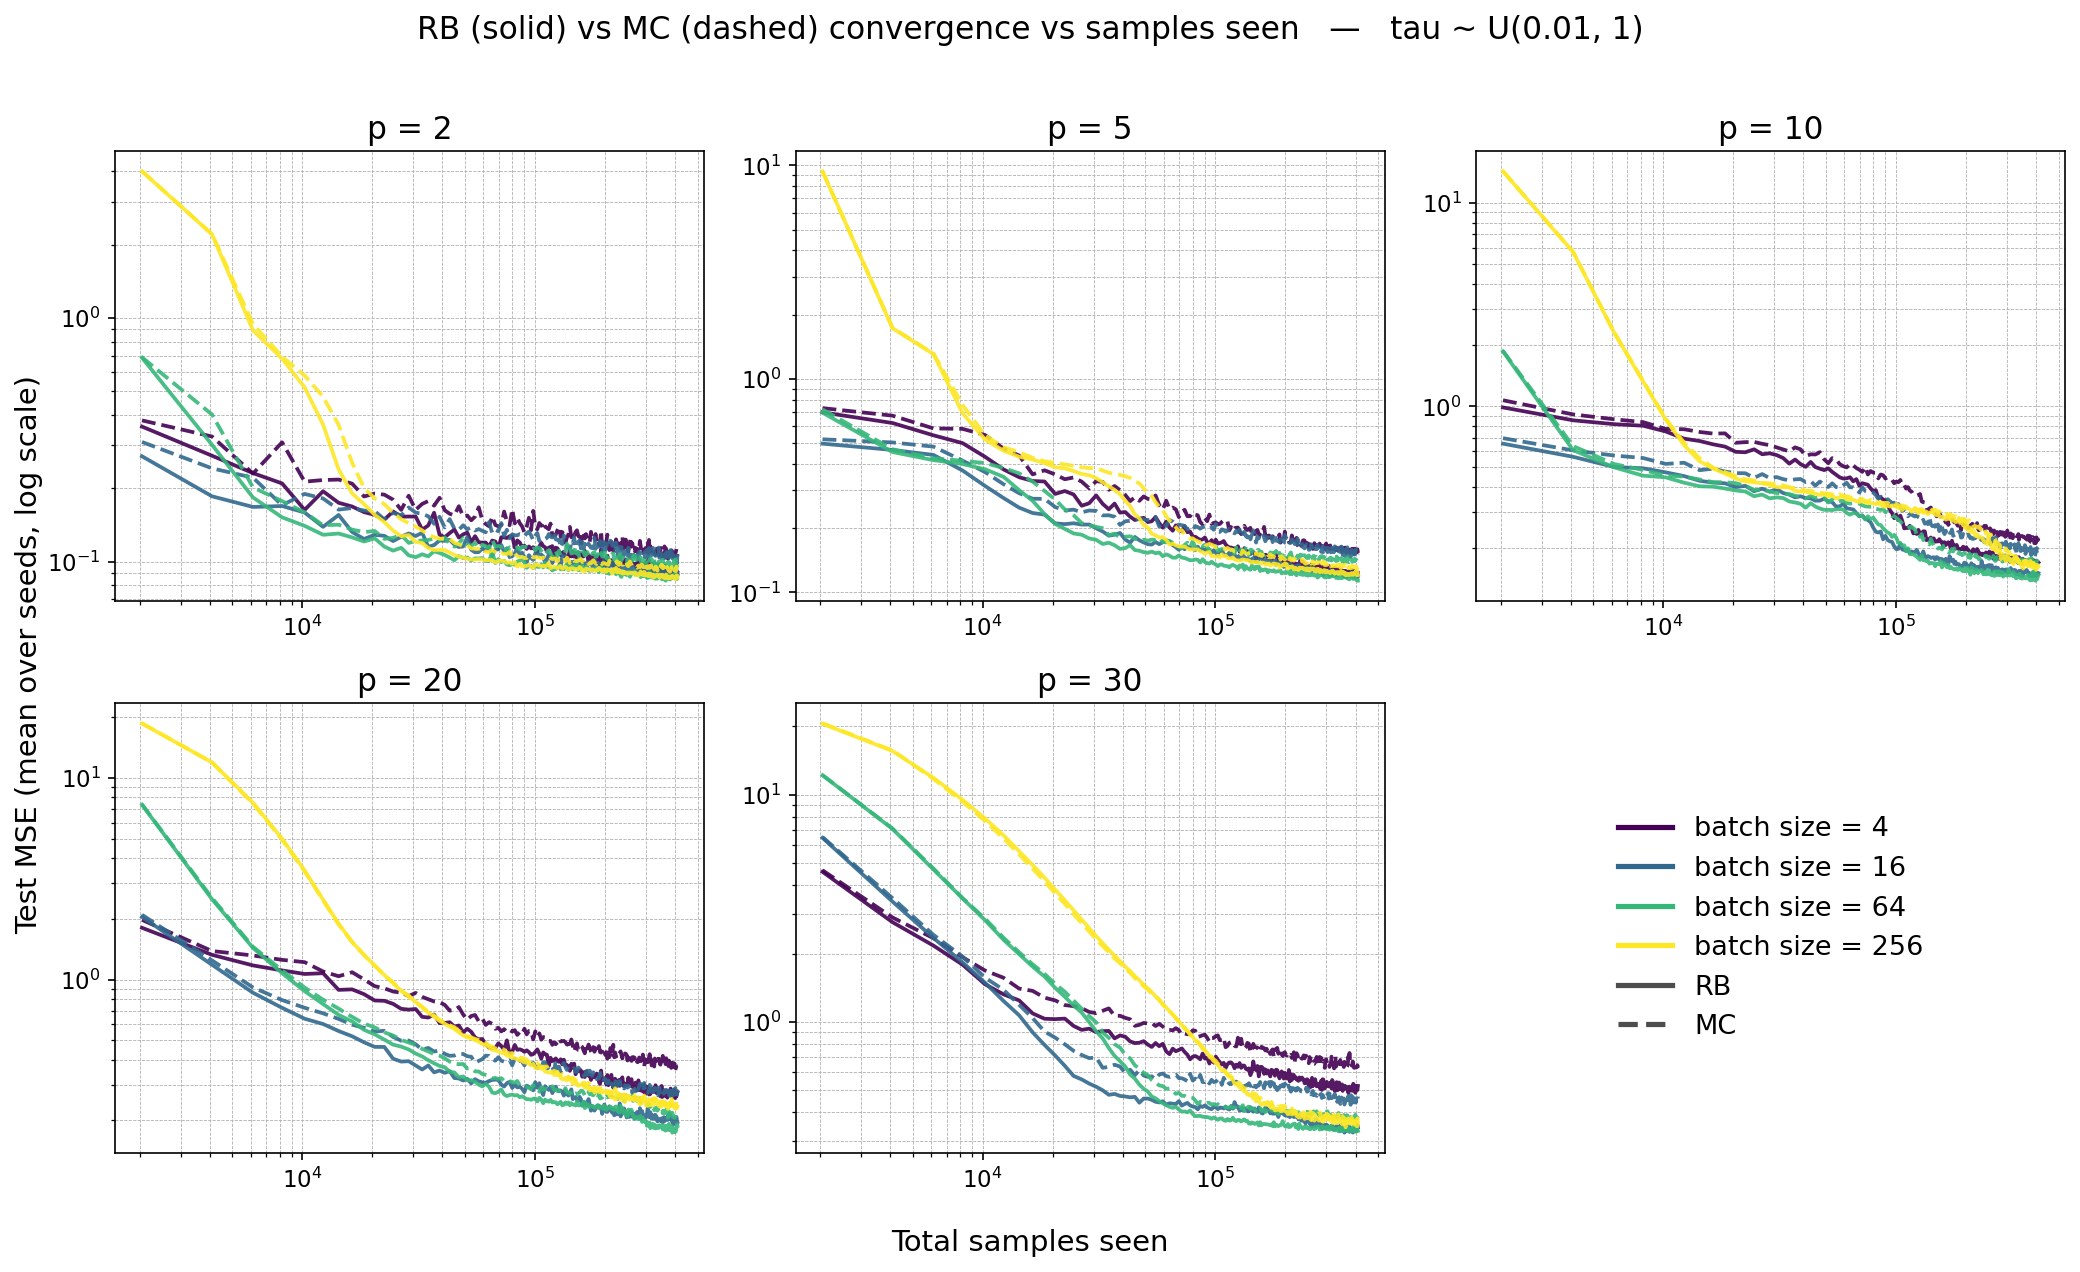
\includegraphics[width=\textwidth]{rb_tau_vs_samples}}
    {\fbox{\parbox[c][4.5cm][c]{\textwidth}{\centering\itshape
      Figure pending: test MSE vs total samples seen
      (re-export \texttt{rb\_tau\_vs\_samples}).}}}
  \caption{Test MSE against the total number of simulated samples seen
  (both axes logarithmic), for parameter dimension
  $p \in \{2, 5, 10, 20, 30\}$ and batch sizes $\{4, 16, 64, 256\}$
  (colours), under $\tau \sim \Uniform(0.01, 1)$. The Rao-Blackwellised
  estimator (solid) lies below the Monte Carlo estimator (dashed) at
  every batch size: it reaches a given accuracy from fewer simulated
  samples, a saving in the dominant cost of training.}
  \label{fig:vs-samples}
\end{figure}

% \subsection{Confirming the noise-level scaling}
% \label{sec:lr-sigma-scaling}

% Equation~\eqref{eq:plateau-gap} predicts that the plateau gap scales
% linearly with $\E[\sigma^2]$. This is tested by comparing two priors
% on $\tau$: the high-noise prior used here and a lower-noise prior used
% in earlier runs. The two differ in $\E[\sigma^2]$ by a factor of
% approximately $55$, and the analysis predicts the plateau gaps to
% differ by the same factor. The measured gaps differ by a factor of
% about $55$ - agreement to one significant figure, which is the
% precision the leading-order analysis of Section~\ref{sec:sgd-plateau}
% can be expected to deliver.

% ----------------------------------------------------------------

\section{Plug-in versus Rao-Blackwellised estimators}
\label{sec:rb-vs-plugin}

Our above analysis of the Rao-Blackwellised loss is built on the existence of an analytical conditional, in the case of linear regression this is $\beta_n(\sigma, \mathbf{y}) = \E[\beta \given \mathbf{y}, \sigma]$. Since this conditional mean is available in closed
form, it is natural to ask whether the network needs a $\beta$-head at all: one
could train it to estimate only the noise scale $\hat{\sigma}_\gamma(\bm y) \approx \E[\sigma \given \mathbf{y}]$ and recover the
coefficients by substitution. This is the \emph{plug-in} estimator,
\begin{equation}
  \tilde{\beta}(\mathbf{y}) = \beta_n\big(\hat{\sigma}_\gamma(\mathbf{y}), \mathbf{y}\big),
\end{equation}
the conditional mean evaluated at a point estimate of $\sigma$. While this estimator will also remove the noise introduced from sampling $\beta$, as we will now show, it is biased.

Let us first define the true posterior mean of the noise scale as $\bar{\sigma} = \E[\sigma \given \mathbf{y}]$ and note the first two moments of the posterior of $\sigma$:
%
\begin{equation*}
  \E_{\sigma\given\mathbf{y}}[\sigma - \bar\sigma] = 0,
  \qquad
  \E_{\sigma\given\mathbf{y}}\big[(\sigma - \bar\sigma)^2\big]
  = \Var(\sigma \given \mathbf{y})
  \label{eq:posterior-moments}.
\end{equation*}
%
Now let us fix $\mathbf{y}$ and expand $\beta_n(\sigma, \mathbf{y})$ to second order about $\bar{\sigma}$:
%
\begin{equation}
  \beta_n(\sigma)
  = \beta_n(\bar\sigma)
    + \beta_n'(\bar\sigma)\,(\sigma - \bar\sigma)
    + \tfrac{1}{2}\,\beta_n''(\bar\sigma)\,(\sigma - \bar\sigma)^2
    + \cdots.
  \label{eq:taylor}
\end{equation}
%
Using \eqref{eq:posterior-moments} and \eqref{eq:taylor}, the bias can be approximated as:
%
\begin{equation}
  \E[\beta \given \mathbf{y}] - \tilde{\beta}(\mathbf{y})
  \;=\;
  \E_{\sigma\given\mathbf{y}}[\beta_n(\sigma)] - \beta_n(\bar\sigma)
  \;\approx\;
  \tfrac{1}{2}\,\beta_n''(\bar\sigma, \mathbf{y})\,\Var(\sigma \given \mathbf{y}),
  \label{eq:plugin-bias}
\end{equation}
%
dropping higher-order terms and treating $\hat\sigma = \bar\sigma$ to
isolate the substitution error. The bias vanishes when $\beta_n$
is affine in $\sigma$ or the posterior of $\sigma$ is degenerate, and otherwise
scales with the curvature of $\beta_n$ and the posterior variance of $\sigma$: it
is the cost of conditioning on a point estimate of $\sigma$ rather than
integrating it out.

In the Bayesian linear regression model that curvature is genuinely present. The conditional mean
\begin{equation*}
  \beta_n(\sigma, \mathbf{y})
  = \big(\sigma_0^{-2} I_p + \sigma^{-2} X^\top X\big)^{-1}
    \sigma^{-2} X^\top \mathbf{y}
\end{equation*}
is a nonlinear, saturating function of the noise scale --- approaching the
least-squares solution $(X^\top X)^{-1} X^\top \mathbf{y}$ as $\sigma \to 0$ and
shrinking towards the prior mean $0$ as $\sigma$ grows --- so
$\beta_n'' \neq 0$ and~\eqref{eq:plugin-bias} does not vanish.

The Rao-Blackwellised estimator does not pay this price, because its
$\beta$-head performs the average in~\eqref{eq:nested-risk} for free. Its
target is the posterior mean $\E[\beta \given \mathbf{y}]$ --- the same as the
standard Monte Carlo head, with which it shares a minimiser by construction
(Section~\ref{sec:rb-bayes-risk}) --- and squared-error training realises that
minimiser as the conditional mean of the target given $\mathbf{y}$. The
marginalisation over $\sigma$ that the plug-in skips is carried out by the
regression itself: across training each $\mathbf{y}$ is paired with the spread of
$\sigma$ its posterior allows, and the fitted value is their average; a point
estimate $\hat\sigma$ carries none of that spread. How much the plug-in loses
therefore depends on how sharply the posterior of $\sigma$ concentrates --- small
where $\sigma$ is well identified, larger where it is not.


\section{Discussion}
\label{sec:lr-discussion}

The experiments support a strong conclusion, that Rao-Blackwellisation of the 
Bayes risk loss does indeed improve training efficiency. The Monte Carlo estimator carries the full gradient
variance, including the large component contributed by the sampled
coefficients $\bm{\beta}$ in the high-noise regime; the
Rao-Blackwellised estimator removes that component analytically,
substituting the conditional posterior mean, and settles markedly
lower. At the baseline cell the Monte Carlo estimator's final loss
sits $119\%$ above the floor and the Rao-Blackwellised estimator's only
$57\%$ above it, closing about half of the Monte Carlo estimator's
excess.

This is the behaviour Section~\ref{sec:rb-loss} predicts. Its gradient-variance result
guarantees that Rao-Blackwellisation cannot raise the variance of the
training gradient, for any model and any architecture, and a
lower-variance gradient is a cleaner signal for the optimiser. The
grid bears this out without exception: across every combination of
seed, parameter dimension, and batch size, the Rao-Blackwellised
estimator reached a lower final loss than the Monte Carlo estimator.

Section~\ref{sec:linear-network} shows that when the network is
linear in its weights, Rao-Blackwellisation reduces the variance not
only of the gradient but of the fitted weights themselves; for a
nonlinear network no such closed-form statement is available. The
estimator trained here is nonlinear, a multilayer perceptron, so that
stronger weight-level guarantee does not formally apply to it. That
Rao-Blackwellisation nonetheless lowers its loss in every cell is
empirical evidence that the linear-case mechanism carries over,
consistent with reading the final layer of the network as a linear
map of fixed features, the regime in which
Section~\ref{sec:linear-network} does apply. 
% ================================================================
%  CHAPTER 5 -- IMPORTANCE SAMPLING: AN AR(1) CASE STUDY
%  Rewrite v4 (discovery-narrative order): bridge from RB -> empirical
%  origin (architecture play, uneven fit) -> the IS idea -> mechanics
%  -> negative result -> diagnosis (why) -> conditions (when) -> contrast.
% ================================================================
\chapter{Importance Sampling}
\label{ch:importance-sampling}

Chapter~\ref{ch:rao-blackwell} reduced the variance of the training
gradient by integrating a conjugate block of the parameter vector out
of the loss. That construction came with a guarantee. The
Rao-Blackwell variance gap~\eqref{eq:variance-gap} is positive
semi-definite, so the construction can never make the gradient noisier,
for any model and any architecture; on Bayesian linear regression it
gave faster convergence and a lower error in every cell of the grid.
This chapter asks whether a second Monte Carlo variance-reduction
technique, \emph{importance sampling}, can help training in the same
way.

The idea came from an experiment rather than from theory. While testing
estimator architectures on a first-order autoregressive model, we
compared the trained network against an exact-posterior reference, and
its accuracy looked uneven across the parameter space. The network
seemed to do worst on the near-non-stationary series at the edges of
the autoregressive coefficient, and on the faint, low-amplitude series
at small noise scale. These are the regions where the realisations are
most distinctive and the process is hardest to simulate, so we suspected
they were also the hardest to estimate. Under a uniform prior, though,
the network sees them no more often than any other part of the
parameter space. Importance sampling offered a way to change that: draw
the training parameters from a proposal that oversamples the difficult
regions, then reweight the loss so that it stays unbiased for the
original prior. If the network's error were concentrated in those
regions, spending more of the simulation budget there should buy
accuracy for the same number of training steps.

The result is negative. Across a family of proposals that oversample
the edges of the parameter space ever more aggressively, the test error
of the trained estimator does not fall; under the most aggressive
proposal it rises, while the effective sample size collapses by more
than an order of magnitude. The negative result is worth reporting
because its cause is specific, and because it contrasts with the
previous chapter. Section~\ref{sec:why} traces the cause to two facts
about the experiment: the trained estimator is already close to the
exact posterior across the whole prior, so little reducible error
remains for any proposal to recover, and the regions we oversampled are
not the ones where its error is largest. Section~\ref{sec:when} sets out
the conditions under which importance sampling does help training, and
why none of them held here. Rao-Blackwellisation never makes training variance worse, for any model and
architecture; importance sampling helps only when the proposal matches
the structure of the problem, and when it does not, the best it can do
is leave the error unchanged.



% ----------------------------------------------------------------
\section{Importance sampling}
\label{sec:is-basics}

Importance sampling is a Monte Carlo technique for estimating an
expectation $\E_{\bm{\theta} \sim p}[f(\bm{\theta})]$ by drawing from a
different distribution $q$ and reweighting:
%
\begin{equation}
  \E_{\bm{\theta} \sim p}[f(\bm{\theta})]
  = \int f(\bm{\theta})\, p(\bm{\theta}) \dd\bm{\theta}
  = \int f(\bm{\theta})\,
      \frac{p(\bm{\theta})}{q(\bm{\theta})}\, q(\bm{\theta}) \dd\bm{\theta}
  = \E_{\bm{\theta} \sim q}\!\left[
      f(\bm{\theta})\,\frac{p(\bm{\theta})}{q(\bm{\theta})}\right].
  \label{eq:is-basic-identity}
\end{equation}
%
The two Monte Carlo estimators,
%
\begin{align}
  \hat{L}_{\mathrm{MC}} &= \frac{1}{N} \sum_{i=1}^{N} f(\bm{\theta}_i), \qquad \bm{\theta}_i \sim p(\bm{\theta}), \\
  \hat{L}_{\mathrm{IS}} &= \frac{1}{N} \sum_{i=1}^{N} w(\bm{\theta}_i)\, f(\bm{\theta}_i), \qquad \bm{\theta}_i \sim q(\bm{\theta}),
\end{align}
%
where $w(\bm{\theta}) = p(\bm{\theta})/q(\bm{\theta})$ is the
\emph{importance weight}, are both unbiased for the same expectation.
The reweighted estimator $\hat{L}_{\mathrm{IS}}$ can have lower variance
than the ordinary estimator $\hat{L}_{\mathrm{MC}}$ when
%
\begin{equation}
  \Var_{\bm{\theta} \sim q}\!\big[w(\bm{\theta})\,f(\bm{\theta})\big]
  < \Var_{\bm{\theta} \sim p}\!\big[f(\bm{\theta})\big].
\end{equation}
%
For a non-negative integrand the proposal that minimises the variance of
$\hat{L}_{\mathrm{IS}}$ is
%
\begin{equation}
  q^{*}(\bm{\theta}) \propto f(\bm{\theta})\,p(\bm{\theta}),
  \label{eq:is-optimal-scalar}
\end{equation}
%
which follows from a Cauchy--Schwarz bound on the second moment of the
reweighted integrand (Appendix~\ref{app:is-optimal-proposal}); under
this proposal the weighted integrand $w(\bm{\theta})f(\bm{\theta})$ is
constant and the variance is zero. Equation~\eqref{eq:is-optimal-scalar}
says to put the proposal mass where the integrand is large, which is
exactly the intuition behind oversampling the hard regions.
Section~\ref{sec:when} returns to this to ask which problems importance
sampling can help; for now it serves as motivation.

In practice the normalising constants of $p$ and $q$ may be unknown, and
the \emph{self-normalised} estimator
%
\begin{equation}
  \hat{r}_{\text{SNIS}}(\bm{\gamma})
  = \frac{\sum_{i=1}^{N} w(\bm{\theta}_i)\,
          L(\bm{\theta}_i, \hat{\bm{\theta}}_{\bm{\gamma}}(\mathbf{y}_i))}
         {\sum_{i=1}^{N} w(\bm{\theta}_i)}
  \label{eq:snis}
\end{equation}
%
is used instead; it is biased at finite $N$ but consistent. To monitor
what a proposal costs we track its \emph{effective sample size}
%
\begin{equation}
  \mathrm{ESS}
  = \frac{\big(\sum_i w(\bm{\theta}_i)\big)^2}{\sum_i w(\bm{\theta}_i)^2}
  = \Big(\textstyle\sum_i \tilde{w}_i^2\Big)^{-1},
  \label{eq:ess}
\end{equation}
%
where $\tilde{w}_i = w(\bm{\theta}_i)/\sum_j w(\bm{\theta}_j)$ are the
normalised weights. It lies between $1$ and $N$ and counts, loosely, how
many of the $N$ reweighted draws carry real weight in the sum. Strictly,
this is the Kish effective sample size of the self-normalised mean: a
convenient proxy for the noise a proposal injects rather than an exact
count of the gradient's effective draws, which
Section~\ref{sec:grad-variance} measures directly. Still, it captures
the price of tilting the proposal away from the prior: when the
effective sample size falls well below $N$, a few draws dominate the
sum, a warning sign that the proposal has been pushed too far from the
prior and may inject more gradient noise than its reweighting removes.

Training a neural Bayes estimator is itself a Monte Carlo integration:
the population loss is the Bayes risk
$r(\bm{\gamma}) = \E_{\bm{\theta}, \mathbf{y}}
[L(\bm{\theta}, \hat{\bm{\theta}}_{\bm{\gamma}}(\mathbf{y}))]$, and each
minibatch estimates its gradient by drawing parameters from the prior.
Drawing $\bm{\theta}$ from a proposal $q$ and reweighting gives the same
risk,
%
\begin{equation}
  r(\bm{\gamma})
  = \int p(\bm{\theta})\,
      \E_{\mathbf{y} \given \bm{\theta}}[L]\dd\bm{\theta}
  = \int \frac{p(\bm{\theta})}{q(\bm{\theta})}\, q(\bm{\theta})\,
      \E_{\mathbf{y} \given \bm{\theta}}[L]\dd\bm{\theta}
  = \E_{\bm{\theta} \sim q}\!\big[w(\bm{\theta})\,
      \E_{\mathbf{y} \given \bm{\theta}}[L]\big].
  \label{eq:is-identity}
\end{equation}
%
The reweighted objective on the right of~\eqref{eq:is-identity} has the
same expectation as the original for every proposal $q$, so the trained
estimator still targets the posterior under the original prior $p$;
reweighting only concentrates the simulation budget where $q$ places
mass. The same identity holds for the gradient that stochastic gradient
descent actually uses, so a proposal changes which parameter values the
gradient is averaged over, not what it estimates.
Section~\ref{sec:when} returns to the question of when this helps.

\section{Application to an AR(1) model}
% ----------------------------------------------------------------
\subsection{The AR(1) model and a recurrent estimator}
\label{sec:ar1-model}

The test model is the first-order autoregressive process of
Example~3, equation~\eqref{eq:ar1}:
$x_t = \rho\,x_{t-1} + \varepsilon_t$ with
$\varepsilon_t \sim \Normal(0, \sigma^2)$, estimand
$\bm{\theta} = (\rho, \sigma)$, priors $\rho \sim \Uniform(-1, 1)$ and
$\sigma \sim \Uniform(0, A)$, and the process initialised from its
stationary distribution $\Normal(0, \sigma^2/(1-\rho^2))$. As
$|\rho| \to 1$ the process approaches non-stationarity, and at
$\rho = 1$ it is a random walk.

Figure~\ref{fig:ar1-examples} shows how the realisations change across
the prior. Persistence grows with the autoregressive coefficient: at
$\rho = 0$ the series is white noise, while near $|\rho| = 1$ it wanders
far from the mean, and the noise scale $\sigma$ sets the amplitude. The
corners of the $(\rho, \sigma)$ box thus produce qualitatively
different, harder-\emph{looking} series than the bulk of the prior. As
the introduction noted, these corners look like where the estimator
should struggle, which makes them the obvious place to spend extra
training draws; Section~\ref{sec:why} shows that for $\rho$ the
appearance is deceptive.

\begin{figure}[t]
  \centering
  \IfFileExists{figures/ar1_examples.png}
    {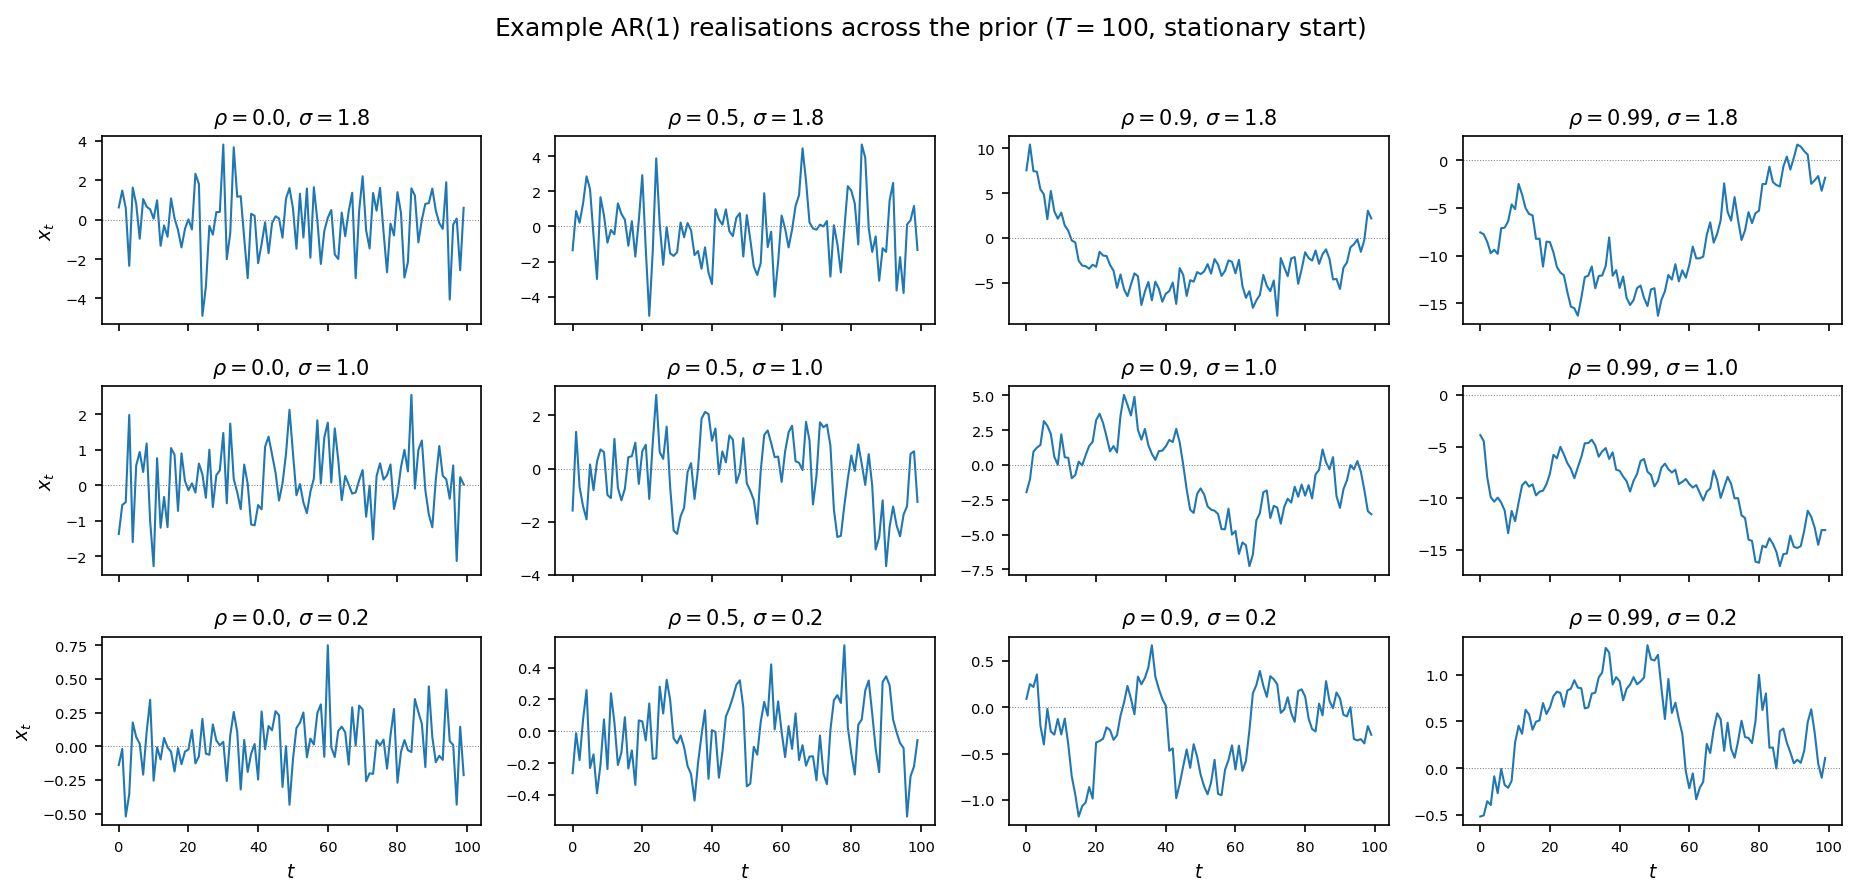
\includegraphics[width=\textwidth]{ar1_examples}}
    {\fbox{\parbox[c][5cm][c]{\textwidth}{\centering\itshape
      Figure pending: example AR(1) realisations
      (run \texttt{ar1\_examples.py}).}}}
  \caption{Example AR(1) realisations across the prior ($T = 100$, from
  the stationary distribution). Persistence grows with $\rho$ (columns):
  white noise at $\rho = 0$, a near-random-walk at $\rho = 0.99$. The
  noise scale $\sigma$ (rows) sets the amplitude.}
  \label{fig:ar1-examples}
\end{figure}

Because the data~\eqref{eq:ar1} are a time series rather than a set of
exchangeable observations, the permutation-invariant DeepSets
architecture of Section~\ref{sec:deepsets} is inappropriate. The
estimator is instead a gated recurrent unit~\citep{cho2014gru}: a
recurrent encoder processes the series, its hidden states are mean
pooled, and a small multilayer perceptron maps the pooled
representation to $(\hat{\rho}, \hat{\sigma})$, with a $\tanh$ output on
the $\rho$-head and a softplus output on the $\sigma$-head to enforce
the parameter constraints. The estimator is trained under squared-error
loss, so by Proposition~\ref{prop:squared-error} it targets the
posterior mean. The series is fed to the encoder on its raw scale,
without standardisation: the amplitude of an AR(1) realisation is set by
$\sigma$, so rescaling each series to unit variance would erase the
scale that identifies $\sigma$, whereas the raw series lets
the network read $\sigma$ off the amplitude and $\rho$ off the
autocorrelation. Both parameters are then identifiable from the input.

To judge the estimator we need a per-dataset gold standard, and the
AR(1) model supplies one: it is conditionally conjugate in both
parameters, so the Gibbs sampler of Section~\ref{sec:cs-ar1} draws from
the exact posterior, and its post-burn-in average is the posterior-mean
reference against which the trained estimator is judged. Comparing the
two is what makes the loss interpretable: it
separates the error the network could in principle train away from the
error that any estimator on the same data must incur.


% ----------------------------------------------------------------
\subsection{A family of proposals}
\label{sec:is-proposals}

With the goal of training our neural network to better fit the edges of the prior, we need a family of proposals that oversample those edges and a single knob that controls how aggressively. For a parameter with bounded support the Beta
distribution provides exactly this. The $\mathrm{Beta}(\alpha, \alpha)$
density on $[0,1]$ is symmetric, and the single parameter $\alpha$
controls where it places mass: $\alpha = 1$ is uniform, $\alpha < 1$ is
U-shaped and concentrates mass at the boundaries, and $\alpha > 1$ is
bell-shaped and concentrates it in the centre. The proposals that target
the difficult-looking boundary take $\alpha < 1$, with $\alpha = 1$ as
the uniform baseline. We also include two proposals on the opposite tilt,
at $\alpha = 1.5$ and $\alpha = 2$; what they do to each coordinate is set
out below.

For the autoregressive coefficient, a draw
$\tilde{\rho} \sim \mathrm{Beta}(\alpha, \alpha)$ on $(0,1)$ is mapped to
$(-1,1)$ by $\rho = 2\tilde{\rho} - 1$; by the change-of-variables
formula the proposal density and importance weight are
%
\begin{equation}
  q(\rho) = \tfrac{1}{2}\,
    \mathrm{Beta}\!\Big(\tfrac{\rho+1}{2};\, \alpha, \alpha\Big),
  \qquad
  w(\rho) = \frac{p(\rho)}{q(\rho)}
  = \frac{1}{\mathrm{Beta}\!\big(\tfrac{\rho+1}{2};\, \alpha, \alpha\big)}.
  \label{eq:is-weight}
\end{equation}
%
At $\alpha = 1$ the Beta density is identically one and $w \equiv 1$,
recovering uniform training. The noise scale is treated differently.
Small $\sigma$ gives a faint, near-white-noise series that looks hard to
pin down, so we oversample only that low-noise tail, as a one-sided test
of whether concentrating draws on a plausibly hard region buys accuracy
there. An asymmetric proposal
$\tilde{\sigma} \sim \mathrm{Beta}(\alpha, 1)$, mapped by
$\sigma = A\tilde{\sigma}$, does this:
%
\begin{equation}
  q(\sigma) = \tfrac{1}{A}\,
    \mathrm{Beta}\!\Big(\tfrac{\sigma}{A};\, \alpha, 1\Big),
  \qquad
  w(\sigma) = \frac{1}{\mathrm{Beta}\!\big(\tfrac{\sigma}{A};\, \alpha, 1\big)},
  \label{eq:is-weight-sigma}
\end{equation}
%
and the joint weight is the product of the two factors. Run at
$\alpha > 1$ instead, the two proposals reverse: the $\rho$-proposal
concentrates on the interior near $\rho = 0$ and the $\sigma$-proposal on
large $\sigma$. We include two such cases, at $\alpha = 1.5$ and
$\alpha = 2$, as the opposite tilt, to
check whether aiming at those regions does any better than aiming at the
boundary. Smaller $\alpha$
oversamples the targeted regions more aggressively but makes $w$ more
variable, which lowers the effective sample size through~\eqref{eq:ess}.
That tension, between concentrating the draws and keeping enough of them
informative, is what the sweep below probes.
Figure~\ref{fig:is-proposals} shows the mechanism: as $\alpha$ falls the
$\rho$-proposal piles mass at both ends $|\rho| \to 1$ and the
$\sigma$-proposal piles mass at small $\sigma$, while the compensating
weights spread over more orders of magnitude.
Figure~\ref{fig:is-samples} makes the same reshaping concrete in the
$(\rho, \sigma)$ plane.

\begin{figure}[t]
  \centering
  \IfFileExists{figures/proposals.png}
    {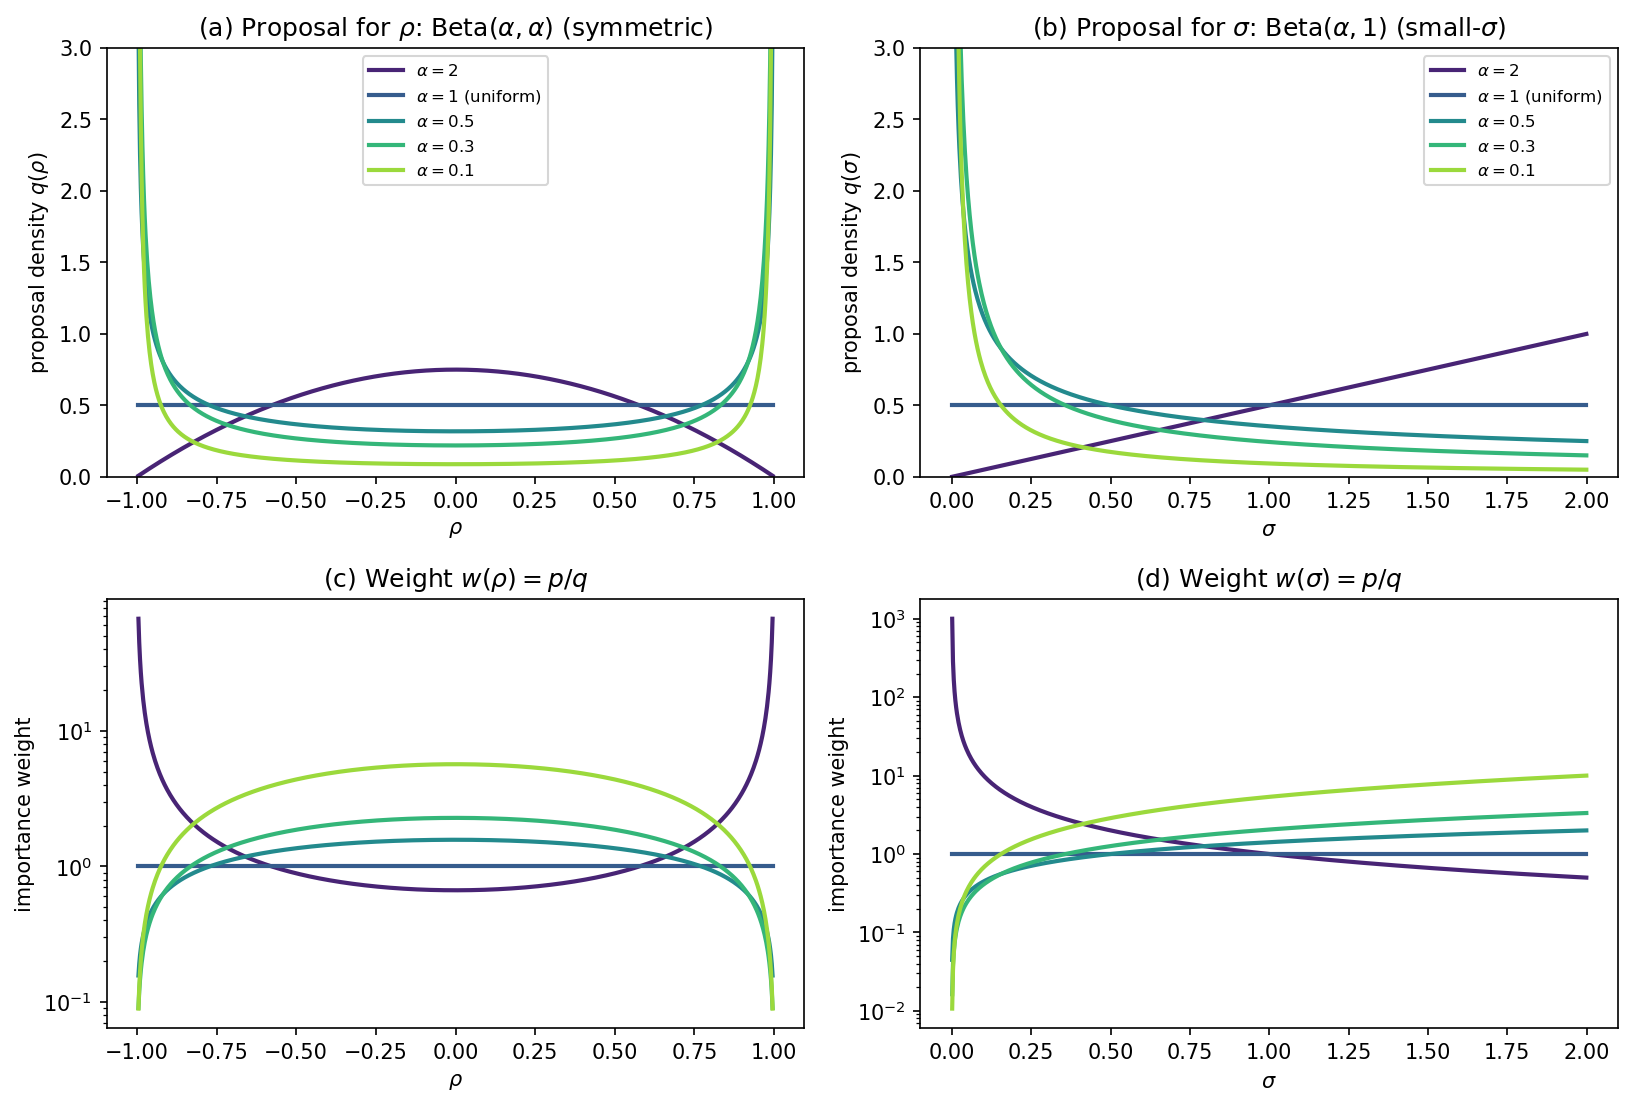
\includegraphics[width=\textwidth]{proposals}}
    {\fbox{\parbox[c][5cm][c]{\textwidth}{\centering\itshape
      Figure pending: proposal densities and importance weights
      (run \texttt{plot\_proposals.py}).}}}
  \caption{The Beta proposal family. \textbf{(a)} The $\rho$-proposal
  $\mathrm{Beta}(\alpha,\alpha)$: $\alpha < 1$ oversamples the boundaries
  $|\rho| \to 1$, $\alpha > 1$ the interior, $\alpha = 1$ is uniform.
  \textbf{(b)} The $\sigma$-proposal $\mathrm{Beta}(\alpha,1)$:
  $\alpha < 1$ oversamples small $\sigma$, $\alpha > 1$ large $\sigma$.
  \textbf{(c, d)} The corresponding importance weights $w = p/q$.}
  \label{fig:is-proposals}
\end{figure}

\begin{figure}[t]
  \centering
  \IfFileExists{figures/samples_weighted.png}
    {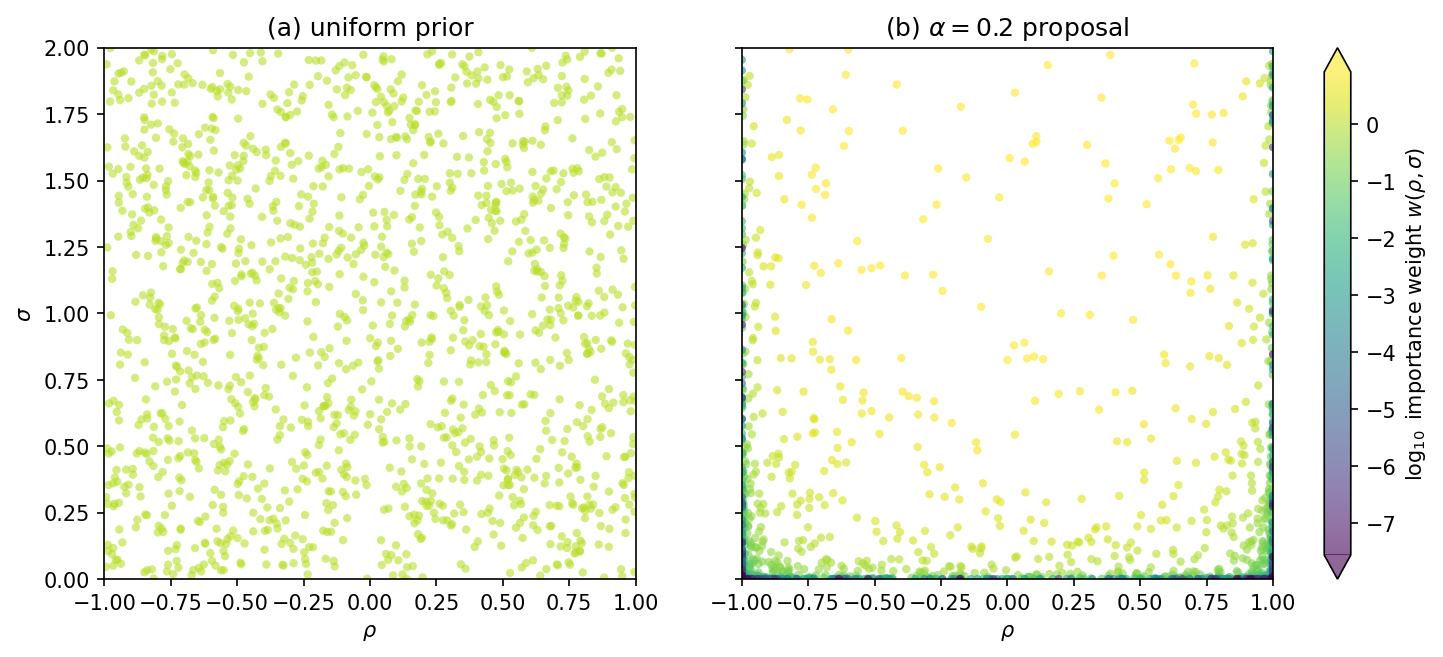
\includegraphics[width=\textwidth]{samples_weighted}}
    {\fbox{\parbox[c][5cm][c]{\textwidth}{\centering\itshape
      Figure pending: $(\rho,\sigma)$ draws coloured by weight
      (run \texttt{plot\_proposals.py}).}}}
  \caption{Training draws in the $(\rho,\sigma)$ plane, coloured by
  importance weight $w$ (log scale). \textbf{(a)} The uniform prior
  ($\alpha = 1$): even draws, unit weights. \textbf{(b)} An aggressive
  proposal ($\alpha = 0.2$): draws cluster on the $|\rho| \to 1$ edges and
  the small-$\sigma$ floor (small weights, dark), leaving the interior and
  large $\sigma$ sparse (large weights, bright).}
  \label{fig:is-samples}
\end{figure}


% ----------------------------------------------------------------
\subsection{Results}
\label{sec:is-results}

Estimators were trained at six proposal strengths,
$\alpha \in \{2.0, 1.5, 1.0, 0.5, 0.3, 0.1\}$: the uniform baseline at
$\alpha = 1$, three increasingly aggressive boundary proposals at
$\alpha < 1$, and two proposals on the opposite tilt at $\alpha = 1.5$ and
$\alpha = 2$. The test error was
broken down over the whole prior and over three regions of interest: the
near-non-stationary boundary $|\rho| > 0.8$, the low-noise region
$\sigma < 0.25A$, and the high-noise region $\sigma > 0.75A$.
Table~\ref{tab:is-sweep} reports the mean squared error in each region
together with the mean effective sample size at each $\alpha$.

\begin{table}[t]
  \centering
  \caption{Test MSE by proposal strength $\alpha$ and region, with the
  mean effective sample size (batch size $256$). Regions: the
  near-non-stationary boundary $|\rho| > 0.8$, low noise
  $\sigma < 0.25A$, and high noise $\sigma > 0.75A$.}
  \label{tab:is-sweep}
  \begin{tabular}{c rrrr r}
    \toprule
    $\alpha$ & all & $|\rho|>0.8$ & low $\sigma$ & high $\sigma$ & ESS \\
    \midrule
    $2.0$ & $0.0181$ & $0.0196$ & $0.0161$ & $0.0245$ & $\phantom{0}93.1$ \\
    $1.5$ & $0.0152$ & $0.0123$ & $0.0121$ & $0.0198$ & $172.7$ \\
    $1.0$ & $0.0136$ & $0.0100$ & $0.0087$ & $0.0187$ & $256.0$ \\
    $0.5$ & $0.0141$ & $0.0102$ & $0.0099$ & $0.0188$ & $155.9$ \\
    $0.3$ & $0.0139$ & $0.0100$ & $0.0084$ & $0.0181$ & $\phantom{0}78.8$ \\
    $0.1$ & $0.0163$ & $0.0128$ & $0.0112$ & $0.0217$ & $\phantom{0}13.4$ \\
    \bottomrule
  \end{tabular}
\end{table}

The result is negative. Across the whole prior the test error is
essentially flat for the baseline and the two milder boundary proposals
($0.0136$, $0.0141$, $0.0139$) and rises at both extremes: climbing through
$\alpha = 1.5$ ($0.0152$) to $0.0181$ at $\alpha = 2$ on one side, and to
$0.0163$ at $\alpha = 0.1$ on the other. No proposal improves on the
uniform baseline. The
regional breakdown (Figure~\ref{fig:is-region}) shows why there is
nothing to redistribute. The low-$\sigma$ region the boundary proposals
oversample is already the easiest at baseline ($0.0087$, the smallest of
the four), and flooding it with draws leaves it there; the high-$\sigma$
region they starve is the hardest ($0.0187$) and stays so; and the
$|\rho| > 0.8$ boundary the $\rho$-proposal targets is among the regions
where the $\rho$-error is smallest. The interior tilts at $\alpha = 1.5$
and $\alpha = 2$ aim the other way, towards the $\rho$-interior and high
$\sigma$, and fare no better: their error is higher in every region, the
high-$\sigma$ region they now oversample included ($0.0245$ at
$\alpha = 2$). The estimator already handles every
region about as well as it can, so reweighting finds no slack to recover,
whichever way it aims. At $\alpha = 0.1$ this is starkest: every region
degrades together, the flooded low-$\sigma$ tail included (it rises from
$0.0087$ to $0.0112$), as the collapsed effective sample size leaves the
gradient too noisy to train well.

\begin{figure}[t]
  \centering
  \IfFileExists{figures/region_breakdown.png}
    {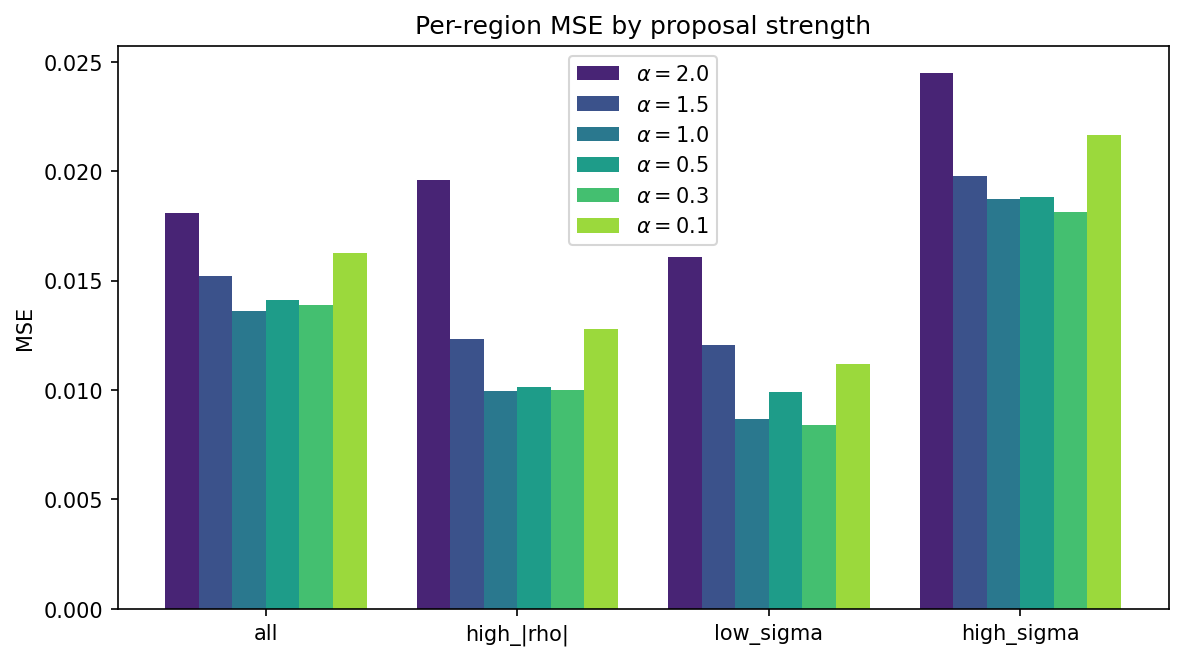
\includegraphics[width=0.85\textwidth]{region_breakdown}}
    {\fbox{\parbox[c][6cm][c]{0.85\textwidth}{\centering\itshape
      Figure pending: per-region MSE bars
      (re-export \texttt{region\_breakdown} from the AR(1) sweep).}}}
  \caption{Test MSE by region for each proposal strength $\alpha$. The
  baseline and the two milder boundary proposals ($\alpha = 1, 0.5, 0.3$)
  sit lowest and together; the interior tilt $\alpha = 1.5$ is intermediate,
  and the extremes $\alpha = 0.1$ and $\alpha = 2$ are worse in every
  region.}
  \label{fig:is-region}
\end{figure}

What does fall is the effective sample size: it peaks at $256$ for the
uniform baseline and drops away as the proposal tilts in either
direction, to $173$ at $\alpha = 1.5$ and $93$ at $\alpha = 2$ on one side
and $13$ at $\alpha = 0.1$ on the other, as the
increasingly variable weights~\eqref{eq:is-weight} let a handful of draws
dominate the reweighted sum. This is the proposal's one reliable effect,
and it is a cost, not a benefit. The training curves
(Figure~\ref{fig:is-curves}) show its consequence: the three milder
proposals converge together near the floor, while $\alpha = 1.5$ settles a
little above them and the two extremes, $\alpha = 0.1$ and $\alpha = 2$,
sit higher still throughout, jitterier and settling at a
higher loss rather than the same one.

\begin{figure}[t]
  \centering
  \IfFileExists{figures/training_curves.png}
    {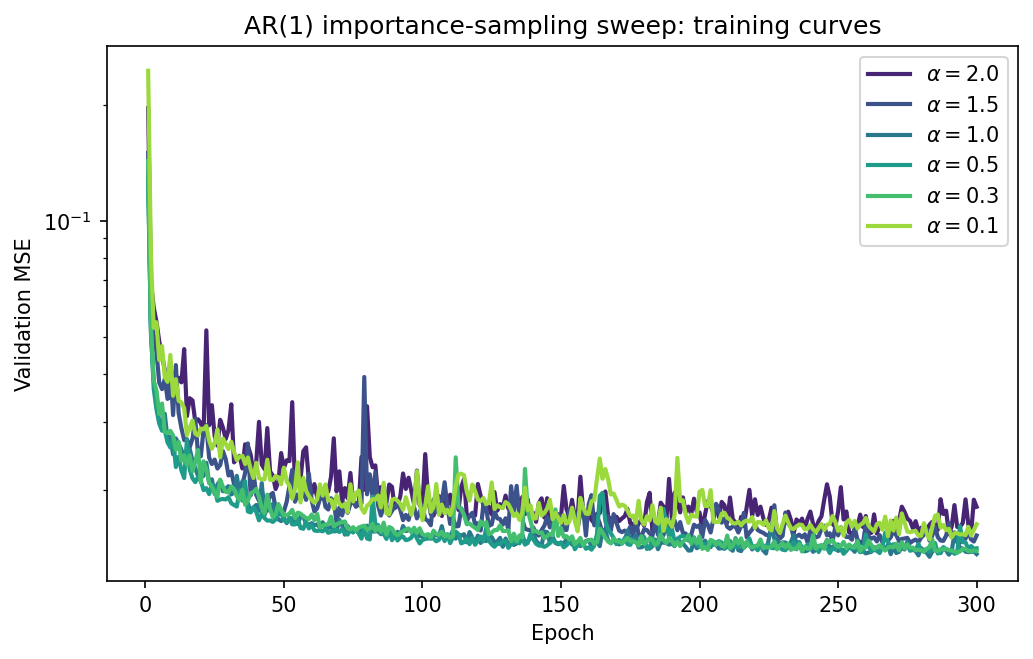
\includegraphics[width=0.8\textwidth]{training_curves}}
    {\fbox{\parbox[c][6cm][c]{0.8\textwidth}{\centering\itshape
      Figure pending: validation MSE training curves
      (re-export \texttt{training\_curves} from the AR(1) sweep).}}}
  \caption{Seed-averaged validation MSE over training for the six
  proposals. The three milder settings ($\alpha = 1, 0.5, 0.3$) converge
  together near the floor; the interior tilt $\alpha = 1.5$ sits a little
  above them, and the extremes $\alpha = 0.1$ and $\alpha = 2$ stay higher
  still, jitterier and settling higher.}
  \label{fig:is-curves}
\end{figure}
\subsection{The gradient variance, measured directly}
\label{sec:grad-variance}

The previous section read the negative result off two indirect quantities: the
test error of the trained estimator, which no proposal lowered, and the
effective sample size, which every proposal lowered. Neither is the quantity
importance sampling is meant to reduce. What training actually consumes is the
gradient: by~\eqref{eq:is-identity} each minibatch estimates
$\nabla_{\bm{\gamma}} r$ by reweighting draws from the proposal, and the
speed of stochastic gradient descent is governed by the variance of that
estimate, not by the variance of the loss nor by the effective sample size on its
own. This section measures the gradient variance directly, and so asks of each
proposal the question the chapter has thus far answered only by proxy: did
reweighting make the gradient less noisy, or more?

The measurement holds the estimator fixed. At a frozen set of weights
$\bm{\gamma}$ and a proposal $q_{\alpha}$, a single minibatch of the common size
$B = 256$ produces the self-normalised gradient
%
\begin{equation}
  \mathbf{g}
  = \nabla_{\bm{\gamma}} \sum_{i=1}^{B} \tilde{w}_i\,
      L(\bm{\theta}_i, \hat{\bm{\theta}}_{\bm{\gamma}}(\mathbf{y}_i)),
  \qquad \bm{\theta}_i \sim q_{\alpha},
  \label{eq:grad-est}
\end{equation}
%
exactly the estimator the training loop applies in~\eqref{eq:snis}. Drawing $M$
independent minibatches, each of the same size $B$ so that every $\alpha$ spends
the identical simulation budget per step, the total gradient variance is
estimated by
%
\begin{equation}
  V(\alpha)
  = \Tr\bigl(\Cov(\mathbf{g})\bigr)
  = \frac{1}{M} \sum_{m=1}^{M}
      \big\lVert \mathbf{g}^{(m)} - \bar{\mathbf{g}} \big\rVert_2^2,
  \qquad
  \bar{\mathbf{g}} = \frac{1}{M} \sum_{m=1}^{M} \mathbf{g}^{(m)},
  \label{eq:grad-var}
\end{equation}
%
the spread of the minibatch gradient about its own mean, summed over every weight
of the network. The quantity reported is the ratio $V(\alpha)/V(1)$ to the
uniform baseline: a value below one is a genuine variance reduction, a value
above one is added noise, and the baseline sits at one by construction. Because
the variance depends on the weights at which it is taken, the comparison is made
at the same network for every proposal: a fresh random initialisation, fixed and
identical across the sweep. Each ratio is averaged over three measurement seeds.

The result is unambiguous (Figure~\ref{fig:grad-variance}). The gradient variance
is smallest at the uniform baseline and rises under every proposal; no setting of
$\alpha$ reduces it, and the inflation grows monotonically as the proposal tilts
further from uniform in either direction. The milder proposals raise it only
gently --- by a factor of about $1.3$ at $\alpha = 0.5$, $2.2$ at $\alpha = 0.3$,
and $2.3$ at the opposite tilt $\alpha = 1.5$ --- while the extremes raise it
sharply, by roughly $14\times$ at $\alpha = 0.1$ and $8.6\times$ at $\alpha = 2$.
This is the direct counterpart of the test-error and effective-sample-size
findings of Section~\ref{sec:is-results}: the one reliable effect of reweighting
here is to make the gradient noisier. No proposal in the Beta family reduced the
variance that training consumes; Section~\ref{sec:why} explains why none
could.
%
\begin{figure}[t]
  \centering
  \IfFileExists{figures/grad_variance.png}
    {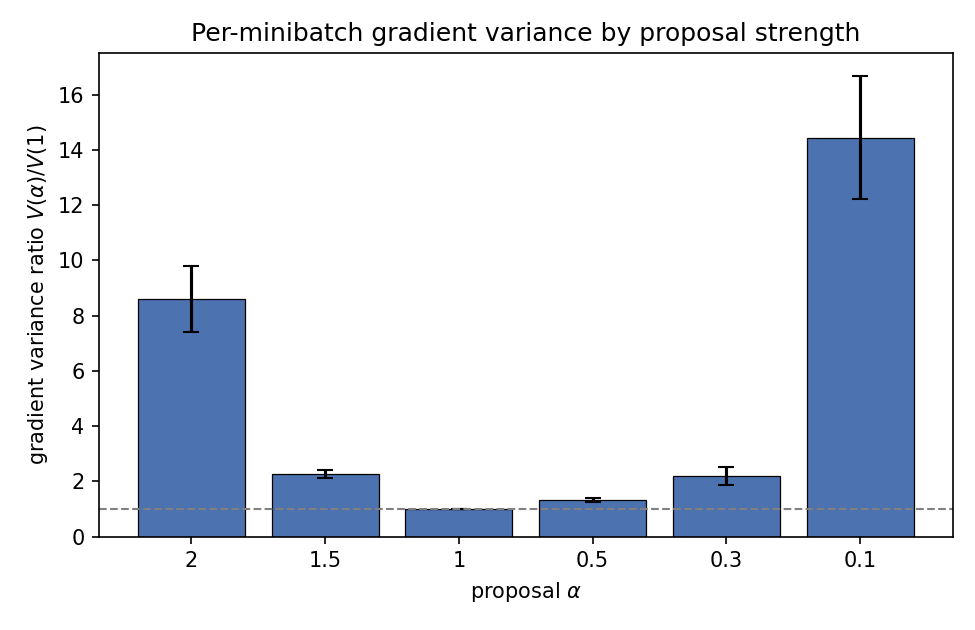
\includegraphics[width=0.8\textwidth]{grad_variance}}
    {\fbox{\parbox[c][6cm][c]{0.8\textwidth}{\centering\itshape
      Figure pending: gradient-variance ratio $V(\alpha)/V(1)$ vs $\alpha$
      (run \texttt{grad\_variance.py}).}}}
  \caption{Per-minibatch gradient variance by proposal strength, as the ratio
  $V(\alpha)/V(1)$ to the uniform baseline, measured at a fresh random
  initialisation and averaged over three seeds (error bars show the seed spread).
  The dashed line marks the uniform baseline at one; every proposal lies above
  it, so none reduces the variance, and the two extremes ($\alpha = 0.1$ and
  $\alpha = 2$) inflate it by roughly an order of magnitude.}
  \label{fig:grad-variance}
\end{figure}


% ----------------------------------------------------------------
\subsection{Why reweighting cannot help here}
\label{sec:why}

Reweighting does not change what the training
objective is, only how noisily each minibatch estimates
it~\eqref{eq:is-identity}, so it can speed training only by making the
gradient less noisy. For that to buy anything, two things must hold: the
estimator must have error left to remove, and the proposal must put its
draws where that error is. On the AR(1) problem neither holds, and both
facts come from comparing the trained network with the exact posterior.

The estimator is already about as accurate as any estimator could be.
Table~\ref{tab:gru-vs-gibbs} compares the GRU with the Gibbs posterior
mean, the Bayes-optimal estimator for this model, on the same test sets.
The GRU's error exceeds the Gibbs error by $22\%$ on the autoregressive
coefficient and $13\%$ on the noise scale.

\begin{table}[t]
  \centering
  \caption{Test MSE of the GRU estimator and the Gibbs posterior-mean
  (Bayes) reference, by parameter, on a held-out test set.}
  \label{tab:gru-vs-gibbs}
  \begin{tabular}{l rr}
    \toprule
             & MSE in $\rho$ & MSE in $\sigma$ \\
    \midrule
    Gibbs posterior mean (Bayes) & $0.0073$ & $0.0056$ \\
    GRU estimator                & $0.0089$ & $0.0063$ \\
    \bottomrule
  \end{tabular}
\end{table}

The error on any one dataset has two parts. One is the posterior
uncertainty that no estimator can remove: even the Bayes-optimal
posterior mean misses, because the data do not pin the parameters down
exactly. The other is the excess the network carries on top, the gap
between it and that optimum. Reweighting cannot touch the first part, and
it recovers the second only where training is held back by gradient
noise, the one thing a cleaner gradient improves. That excess is small in
absolute terms (Table~\ref{tab:gru-vs-gibbs}), and
Figure~\ref{fig:sigma-failure} shows what it is: on the hardest series the
GRU and the Gibbs sampler miss together, so the error there is posterior
uncertainty, not a deficit a better-aimed gradient could close. Little of
the error anywhere is the kind a proposal could recover.

\begin{figure}[t]
  \centering
  \IfFileExists{figures/gibbs_vs_nn.png}
    {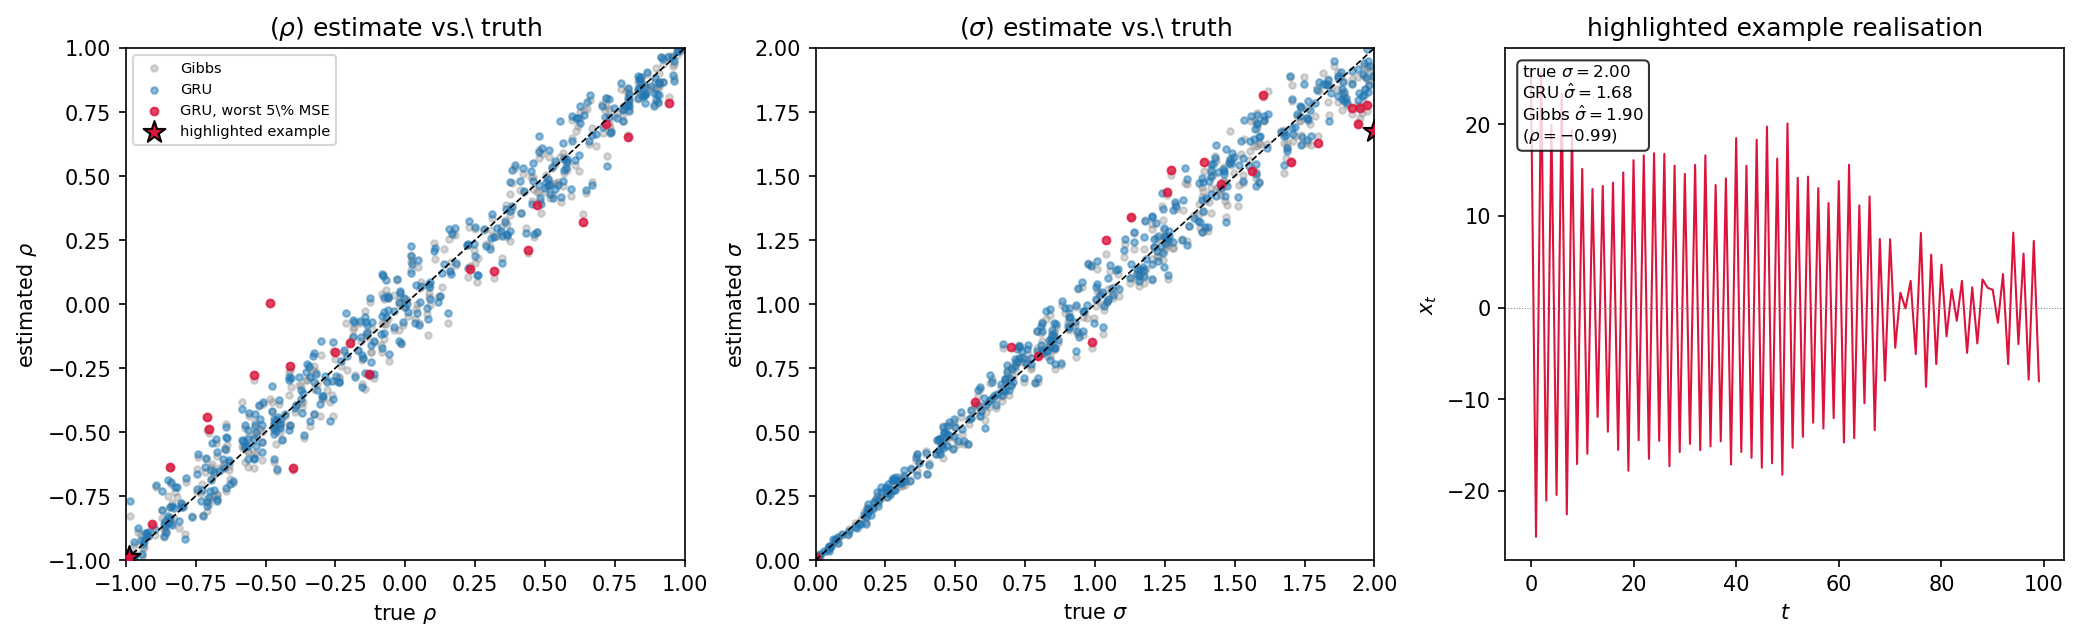
\includegraphics[width=\textwidth]{gibbs_vs_nn}}
    {\fbox{\parbox[c][5.5cm][c]{\textwidth}{\centering\itshape
      Figure pending: GRU versus Gibbs estimates by parameter
      (run \texttt{gibbs\_vs\_nn.py}).}}}
  \caption{Estimates from the baseline GRU (blue) and the Gibbs posterior
  mean (grey) against the truth, for $\rho$ (left) and $\sigma$ (centre);
  the worst-MSE cases are red. Right: one of them as a realisation, an
  extreme series with $\rho \approx -0.99$ and $\sigma$ at the top of its
  range. The GRU recovers $\rho$ exactly, though the series looks the
  hardest of all; both it and Gibbs underestimate the extreme $\sigma$, so
  that residual is shared with the Bayes-optimal sampler, not something the
  network could train away.}
  \label{fig:sigma-failure}
\end{figure}

The little error that remains sits in the opposite place from where the
proposals aim. Figure~\ref{fig:binned-mse}
bins the test error by each parameter. The error in $\rho$ is largest in
the interior, near $\rho = 0$, and smallest at the boundaries
$|\rho| \to 1$, the very edge the $\rho$-proposal floods; it is also
raised where $\sigma$ is small. The error in $\sigma$ runs the other way,
growing with $\sigma$, so the high-noise end carries most of it while the
low-$\sigma$ tail the $\sigma$-proposal floods is the cleanest part.

There is a clean reason the boundary is the easy end for $\rho$.
Estimating $\rho$ is a regression of each $x_t$ on its lag $x_{t-1}$, so
the posterior variance of the slope is the noise variance over the spread
of the predictor, $\Var(\rho \mid \sigma^2, \mathbf{x}) = \sigma^2/S$ with
$S = \sum_t x_{t-1}^2$ (Section~\ref{sec:cs-ar1}). The series starts from
its stationary distribution, of variance $\sigma^2/(1-\rho^2)$, so
$S \approx T\sigma^2/(1-\rho^2)$ and the posterior variance is
$\approx (1-\rho^2)/T$. As $|\rho| \to 1$ the series makes larger, more
persistent excursions, and this variance vanishes: the data pin $\rho$
down most tightly exactly where the series looks most dramatic. The
motivating intuition mistook one kind of difficulty for another: a
near-non-stationary series has large
swings that carry the most information about $\rho$, so it is the
\emph{easiest} to estimate $\rho$ from. The hard-to-simulate end and the
hard-to-estimate end are opposite.

\begin{figure}[t]
  \centering
  \IfFileExists{figures/binned_mse.png}
    {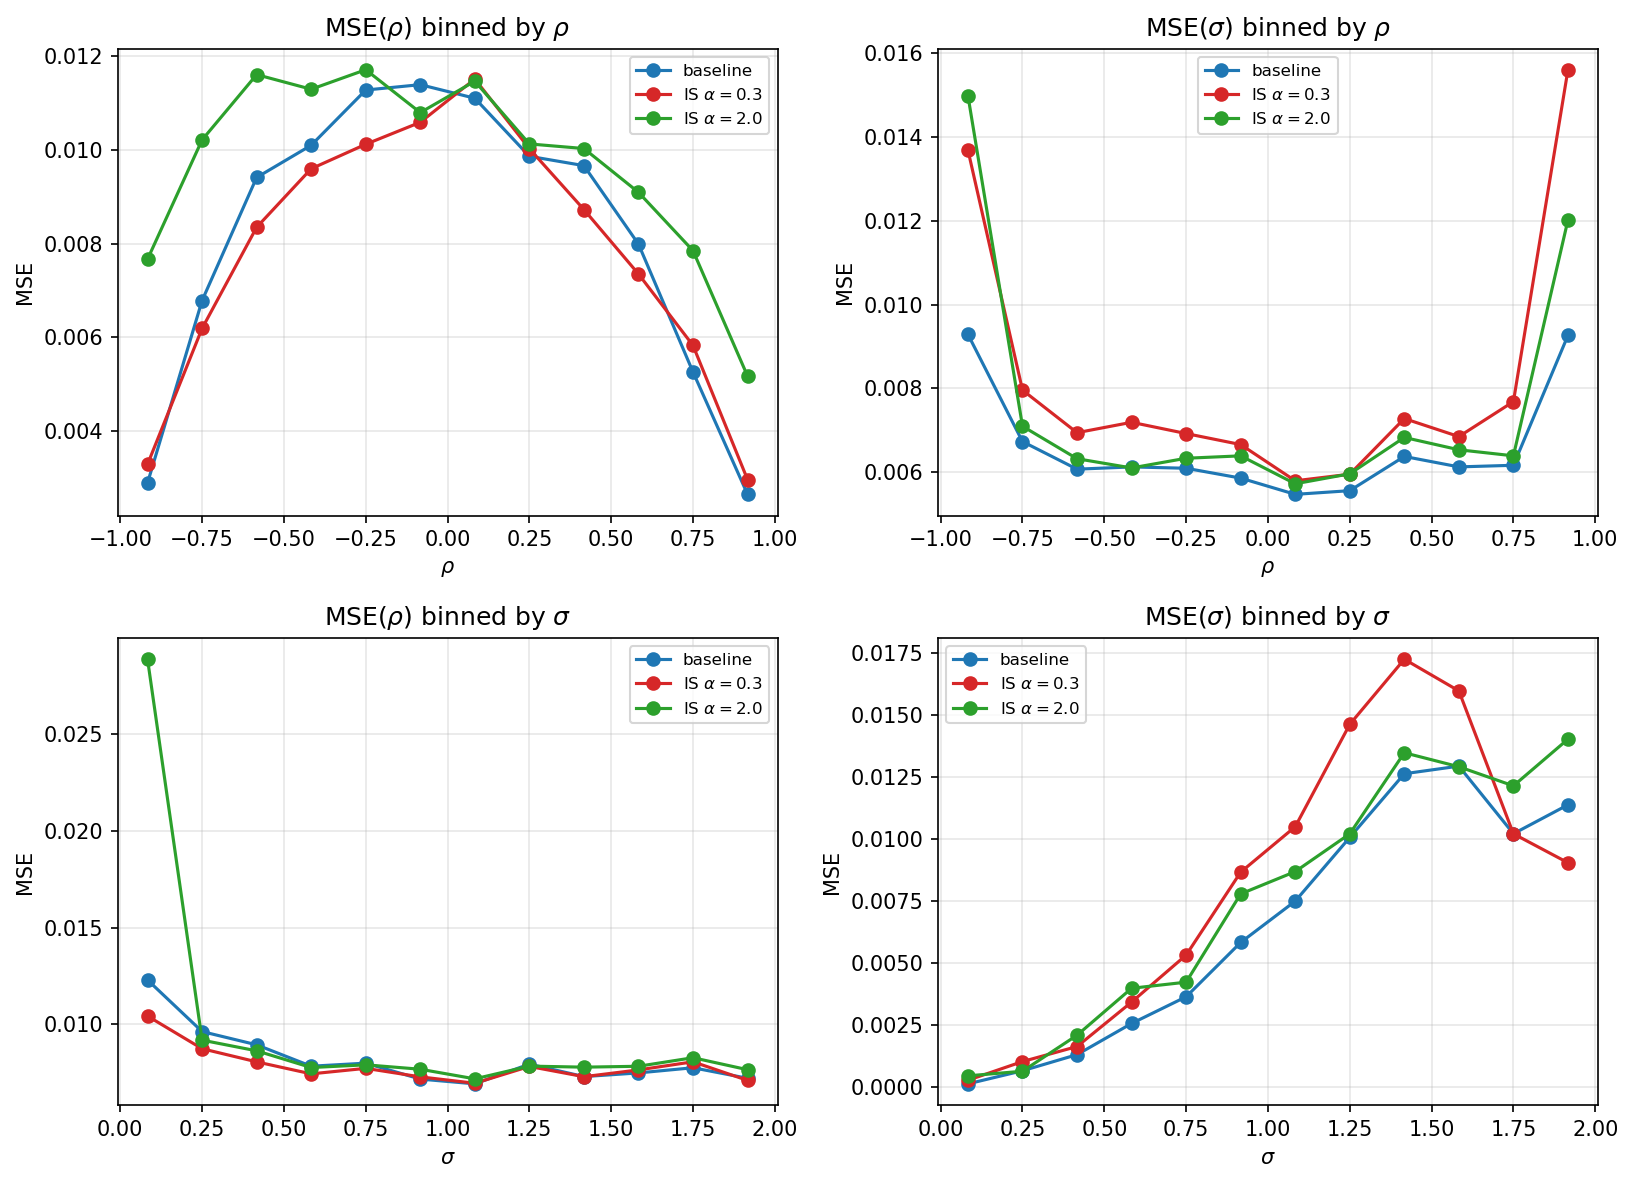
\includegraphics[width=\textwidth]{binned_mse}}
    {\fbox{\parbox[c][5.5cm][c]{\textwidth}{\centering\itshape
      Figure pending: test MSE binned by parameter
      (run \texttt{extra\_figures.py}).}}}
  \caption{Test error binned by $\rho$ (top row) and by $\sigma$ (bottom
  row), for the baseline (blue), the boundary proposal $\alpha = 0.3$
  (red), and the opposite tilt $\alpha = 2$ (green). The error lives in
  the $\rho$-interior and at large $\sigma$, not at the boundary or
  low-$\sigma$ tail the proposals target; neither overlay improves on the
  baseline.}
  \label{fig:binned-mse}
\end{figure}

The $\alpha = 2$
proposal puts its draws in the $\rho$-interior and at high $\sigma$, where
the error genuinely is largest, and it is no better than the rest
(Table~\ref{tab:is-sweep}), because the error there is the irreducible
kind the Gibbs sampler shares. So no setting of the Beta family helps:
where the error is large it cannot be removed, and where it can be removed
it is already small.

Against these absent gains stands a cost that is always paid. The more a
proposal concentrates its draws, the more variable its
weights~\eqref{eq:is-weight}, the lower the effective sample
size~\eqref{eq:ess}, and the noisier the gradient left by the
self-normalised objective~\eqref{eq:snis}. With no gain to offset it, this
cost is the whole effect: at $\alpha = 0.1$ it shows up as the
across-the-board degradation of Section~\ref{sec:is-results}. Reweighting
here can only add noise, and the harder it is pushed, the more it adds.


% ----------------------------------------------------------------
\section{When importance sampling can help}
\label{sec:when}


The negative result is therefore a verdict on a mismatch, not on importance sampling in general. Three conditions separate the problems in which importance sampling can help from those in which it cannot.

The first is that there must be reducible error left to recover. Section~\ref{sec:why} showed that little such error remains in the AR(1) experiment: the trained GRU is already close to the Gibbs posterior-mean reference. The remaining test error is therefore dominated by posterior uncertainty rather than by a failure of optimisation. Reweighting the training distribution cannot remove this irreducible part of the Bayes risk.

The second condition is that the proposal must target where the useful gradient signal is concentrated, not merely where the raw loss is large. For squared-error loss,
\[
L = \|\hat{\bm{\theta}}_{\bm{\gamma}}(\mathbf{y})-\bm{\theta}\|_2^2,
\qquad
\nabla_{\bm{\gamma}} L = 2\left(\nabla_{\bm{\gamma}}\hat{\bm{\theta}}_{\bm{\gamma}}(\mathbf{y})\right)^{\!\top}\left(\hat{\bm{\theta}}_{\bm{\gamma}}(\mathbf{y})-\bm{\theta}\right).
\]

Thus, ignoring variation in the estimator sensitivity $(\|\nabla_{\bm{\gamma}}\hat{\bm{\theta}}_{\bm{\gamma}}(\mathbf{y})\|)$, the gradient magnitude scales like $\sqrt{L}$, not like $L$ itself. A proposal designed to reduce gradient variance should therefore be guided by the size of the gradient contribution, roughly $q \propto p\sqrt{L}$, rather than by the loss alone. More importantly, the relevant loss is the reducible excess over the Bayes estimator. Large loss caused by posterior uncertainty produces noisy residuals, but not a systematic gradient direction that the network can train away.

The third condition is that the variance affected by the proposal must be the dominant source of training noise. Importance sampling changes how often different parameter values $\bm{\theta}$ are drawn, but it does not remove the randomness from simulating a fresh dataset $(\mathbf{y}\mid\bm{\theta})$. If that conditional simulation noise dominates the minibatch gradient, then even a well-aimed proposal can only produce a limited gain.

The proposals used here were fixed in advance by the single parameter
$\alpha$, which cannot know where the recoverable gradient signal lies; on
this problem it aimed badly. One direction for future work is to adapt the
proposal during training, estimating where the gradient is largest as
training proceeds and reshaping $q \propto p\sqrt{L}$ towards it, so that
the simulation budget follows the signal rather than a fixed guess.
Whether such a scheme can realise even the bounded gains these conditions
allow, without its own overhead and instability, is an open question.
A second is to test the method on a problem built to meet the conditions rather than to fail them, where the loss is sharply uneven, the estimator's sensitivity varies in the same direction, and the
residual error is genuinely reducible. That would be the fair positive
counterpart to the AR(1) case study, and the place to further investigate whether
importance sampling can meaningfully help neural Bayes training.


% ----------------------------------------------------------------
\section{Discussion}
\label{sec:is-discussion}

The experiment returns a negative result, and the negative result is the
point. On the AR(1) model, importance sampling with Beta proposals leaves
the trained estimator's test error unchanged for the milder proposals and
raises it at both extremes, all while collapsing the effective sample size
by more than an order of magnitude. Section~\ref{sec:why} explains why:
the estimator is already close to the Bayes reference everywhere, so
little reducible error remains for any proposal to recover, and the
regions the boundary proposals target are the ones the estimator already
handles best. The motivating intuition confused the conspicuous regions,
the ones that are dramatic to look at and awkward to simulate, with the
difficult ones; for the autoregressive coefficient the two are opposite.

Section~\ref{sec:when} turns that failure into a specification: importance
sampling helps training only when there is reducible error to recover,
when the proposal is aimed where the gradient signal actually
concentrates, and when the simulation noise is not what limits training. A
scale-estimation problem can be built to meet these conditions, where the
gain is real if modest; the AR(1) study met none of them where its
proposals aimed.

This is the genuine contrast with Chapter~\ref{ch:rao-blackwell}. The
Rao-Blackwell variance gap~\eqref{eq:variance-gap} is positive
semi-definite for every model and every architecture: the technique
cannot make training variance worse, and on Bayesian linear regression it made
training reliably and substantially better. Importance sampling carries
no such guarantee. It helps only when the proposal is well matched and
gradient noise is the binding constraint; when the difficulty lies
elsewhere, as here, the best it can do is leave the error untouched, and
pushed harder it makes the error worse, while its cost in effective sample
size is paid either way. Both are instances of Monte Carlo variance
reduction applied to estimator training, but they differ in reliability:
one unconditional, the other contingent on a match between the proposal
and the structure of the problem. That difference is the main lesson of
this chapter.
% ================================================================
%  CHAPTER 6 -- DISCUSSION AND CONCLUSION
%  Status: DRAFT v1 (2026-05-18).
% ================================================================
\chapter{Discussion and Conclusion}
\label{ch:conclusion}

% ----------------------------------------------------------------


This thesis began from a single observation: training a neural Bayes
estimator involves Monte Carlo integration of the Bayes risk, and the
gradient that drives training is therefore a Monte Carlo estimator
with a variance. That variance is a property of how the loss is
sampled, not of the inference problem, and it can be reduced.

The primary reduction attempted here is the Rao-Blackwellised loss. When a
block of the parameter vector has a tractable conditional posterior,
that block is integrated out of the loss analytically rather than
sampled. For squared-error loss this amounts to substituting the
conditional posterior mean for the sampled target, with the residual
conditional variance entering only as a constant that does not affect
the gradient. The resulting training gradient is the
Rao-Blackwellisation of the standard one, and the law of total
variance gives a positive semi-definite gradient-variance gap: the
technique can never increase the variance of the training gradient.
For a linear network the guarantee strengthens to the fitted weights
themselves.

The empirical study on Bayesian linear regression bore this out. The
Rao-Blackwellised estimator attained a lower loss than the standard
estimator in every cell of the experimental grid, closed about half
the gap between the standard estimator and the Bayes-optimal floor at
the baseline, and matched the standard estimator's accuracy at a
quarter of the batch size.


Chapter~\ref{ch:importance-sampling} placed Rao-Blackwellisation
alongside importance sampling, a second variance-reduction technique
acting on the training of the estimator. The comparison is the
clearest summary of what makes Rao-Blackwellisation attractive.
Importance sampling can in principle sharpen estimation by
oversampling the regions that contribute most to the loss, but only
when the bottleneck on training is gradient noise and the proposal is
matched to it. On the autoregressive model neither condition held: the
trained estimator already sat close to the Bayes-optimal floor across
the prior, and the proposal oversampled the very regions it handled
best, so reweighting found no error worth recovering and, pushed hard,
only added gradient noise.
Rao-Blackwellisation carries an unconditional guarantee, the
variance gap being positive semi-definite for every model and
architecture, at the cost of requiring a tractable conditional
posterior. Where that conditional structure is present, as it is in
any conditionally conjugate hierarchical model, Rao-Blackwellisation
is the safer and stronger of the two.

One distinction underlies this comparison and is worth stating
directly. Reducing the variance of the loss --- or, more precisely, of
the gradient that drives training --- is not really the primary goal;
the goal is reducing the variance of the estimate that training
produces, the fitted weights $\hat{\bm{\gamma}}$ and the estimator they
define. A cleaner gradient is valuable only insofar as it yields a less
variable estimator. At this level the two techniques separate most
sharply. For a linear network, Section~\ref{sec:linear-network} showed
that Rao-Blackwellisation reduces not only the variance of the gradient
but the variance of the fitted weights themselves, with the last-layer
argument suggesting the same holds approximately for nonlinear
networks. Importance sampling admits no such statement: it bears, and
only contingently, on the variance with which a minibatch estimates the
gradient, and nothing in it carries through to the variance of the
estimator that training returns. That a guarantee can be carried to the
fitted weights for one technique and not the other is the deepest form
of the contrast between them.


Several limitations bound the results. The Rao-Blackwellised loss
requires a tractable conditional posterior for the integrated block;
where no parameter block is conditionally conjugate the construction
does not apply, and only the sampled block benefits when one block is.
The experimental evidence is confined to two models (linear
regression with a multilayer perceptron, and an autoregressive process
with a recurrent network) and does not establish how the method
behaves for richer simulators or larger architectures. The estimators
studied are point estimators and provide no quantification of
posterior uncertainty.

% ----------------------------------------------------------------
\section{Future work}
\label{sec:future-work}

Several directions follow naturally. The linear-network result of
Section~\ref{sec:linear-network} suggests, but does not prove, a
corresponding statement for fully nonlinear networks; making the
last-layer argument rigorous, or bounding its error, would close that
gap. The squared-error construction of Section~\ref{sec:rb-mse} could
be extended to other losses (the quantile loss of
Section~\ref{sec:loss-summaries}, for instance) to Rao-Blackwellise
estimators of posterior quantiles rather than means. Where a parameter
block is only approximately conjugate, a partial or approximate
Rao-Blackwellisation may still reduce variance, and quantifying the
resulting bias--variance trade-off is an open question. The
variance-reduction toolbox of Monte Carlo contains further techniques
not explored here (control variates, antithetic sampling, and
stratified proposals among them), and a systematic comparison of
these against Rao-Blackwellisation for estimator training, including
how they might be combined, is a natural direction. A related
direction is the reparameterisation of the estimator's outputs to
decouple weakly identified parameters, an alternative to variance
reduction for the boundary difficulties of
Chapter~\ref{ch:importance-sampling}. Most importantly, the method
should be tested on the larger, less tractable simulators that are the
natural setting for simulation-based inference.

% ----------------------------------------------------------------
\section{Conclusion}
\label{sec:final}

Neural Bayes estimators amortise Bayesian inference by replacing
per-dataset sampling with a single trained mapping. Because their
training is itself Monte Carlo integration, the variance-reduction
toolbox of Monte Carlo applies to the training loop. This thesis has
shown that Rao-Blackwellisation, in particular, is a cheap and
reliable lever: where a parameter block is conditionally conjugate,
integrating it out of the loss provably reduces the variance of the
training gradient, and in the regimes studied it drives the trained
estimator substantially closer to the Bayes-optimal floor. Conditional
conjugacy, long exploited to make Gibbs sampling possible, turns out
to be equally useful for training the estimators that aim to replace
it.


% ================= BACK MATTER =================
\appendix
% ================================================================
%  APPENDICES
%  Status: DRAFT. Appendix B populated from sweeps2/ (tau-uniform
%  sweep) + floors_and_tables.py (Gibbs floors).
% ================================================================

\chapter{Derivations}
\label{app:derivations}

% ----------------------------------------------------------------
\section{Detailed balance for Metropolis--Hastings}
\label{app:mh-detailed-balance}

This appendix verifies the claim of Section~\ref{sec:metropolis-hastings}
that the Metropolis--Hastings chain satisfies detailed balance with
respect to the posterior $\pi(\bm{\theta}) = p(\bm{\theta} \given
\mathbf{y})$. The transition kernel has an accepted-move component and
a rejected-move component,
%
\begin{equation}
  T(\bm{\theta}' \given \bm{\theta})
  = q(\bm{\theta}' \given \bm{\theta})\,
    \alpha(\bm{\theta}, \bm{\theta}')
  + \delta(\bm{\theta}' - \bm{\theta})\,r(\bm{\theta}),
\end{equation}
%
where $\delta$ is the Dirac delta and
$r(\bm{\theta}) = \int [1 - \alpha(\bm{\theta},
\bm{\theta}'')]\,q(\bm{\theta}'' \given \bm{\theta})
\dd\bm{\theta}''$ is the total rejection probability. For
$\bm{\theta}' = \bm{\theta}$ detailed balance holds trivially, so take
$\bm{\theta}' \neq \bm{\theta}$, where the delta term vanishes.
Substituting the acceptance probability~\eqref{eq:mh-acceptance},
%
\begin{align}
  T(\bm{\theta}' \given \bm{\theta})\,\pi(\bm{\theta})
  &= q(\bm{\theta}' \given \bm{\theta})\,
     \pi(\bm{\theta})\,
     \min\!\left(1,\;
     \frac{\pi(\bm{\theta}')\,q(\bm{\theta} \given \bm{\theta}')}
          {\pi(\bm{\theta})\,q(\bm{\theta}' \given \bm{\theta})}
     \right)
     \notag \\[2pt]
  &= \min\!\Big(
     q(\bm{\theta}' \given \bm{\theta})\,\pi(\bm{\theta}),\;
     q(\bm{\theta} \given \bm{\theta}')\,\pi(\bm{\theta}')
     \Big)
     \notag \\[2pt]
  &= q(\bm{\theta} \given \bm{\theta}')\,\pi(\bm{\theta}')\,
     \min\!\left(
     \frac{\pi(\bm{\theta})\,q(\bm{\theta}' \given \bm{\theta})}
          {\pi(\bm{\theta}')\,q(\bm{\theta} \given \bm{\theta}')},\;
     1\right)
     \notag \\[2pt]
  &= T(\bm{\theta} \given \bm{\theta}')\,\pi(\bm{\theta}'),
\end{align}
%
where the second equality moves the positive factor
$q(\bm{\theta}' \given \bm{\theta})\,\pi(\bm{\theta})$ inside the
minimum and the third moves the positive factor
$q(\bm{\theta} \given \bm{\theta}')\,\pi(\bm{\theta}')$ back out. The
second line is symmetric under exchange of $\bm{\theta}$ and
$\bm{\theta}'$, which is what the third line exploits. Detailed
balance holds, so $\pi$ is the stationary distribution of the chain.

% ----------------------------------------------------------------
\section{The optimal importance sampling proposal}
\label{app:is-optimal-proposal}

This appendix proves the claim of Section~\ref{sec:is-basics} that, among
all proposals $q$, the variance of the importance sampling estimator
$\hat{L}_{\mathrm{IS}}
= \frac{1}{N}\sum_{i} w(\bm{\theta}_i)\,f(\bm{\theta}_i)$, with weight
$w(\bm{\theta}) = p(\bm{\theta})/q(\bm{\theta})$, is minimised by
%
\begin{equation}
  q^*(\bm{\theta}) \propto |f(\bm{\theta})|\, p(\bm{\theta}).
  \label{eq:app-is-optimal}
\end{equation}

\begin{proof}
Since $\hat{L}_{\mathrm{IS}}$ is unbiased for every $q$, minimising its
variance is equivalent to minimising the second moment of a single term,
\begin{equation}
  \E_q\!\left[\left(\frac{f(\bm{\theta}) p(\bm{\theta})}{q(\bm{\theta})}\right)^2\right]
  = \int \frac{f(\bm{\theta})^2 p(\bm{\theta})^2}{q(\bm{\theta})}\, \dd\bm{\theta}.
\end{equation}
By the Cauchy--Schwarz inequality, for any density $q$,
\begin{equation}
  \int \frac{f^2 p^2}{q}\,\dd\bm{\theta}
  = \left(\int \frac{f^2 p^2}{q}\,\dd\bm{\theta}\right)\!\!\left(\int q\,\dd\bm{\theta}\right)
  \geq \left(\int |f|\, p\, \dd\bm{\theta}\right)^2,
\end{equation}
with equality if and only if $f^2 p^2 / q \propto q$, that is,
\begin{equation}
  q^*(\bm{\theta}) \propto |f(\bm{\theta})|\, p(\bm{\theta}).
\end{equation}
The lower bound $\left(\int |f| p\, \dd\bm{\theta}\right)^2$ is independent of $q$,
so $q^*$ attains it and is therefore optimal. When $f \geq 0$ the resulting
weighted integrand $w(\bm{\theta}) f(\bm{\theta})$ is constant, and the variance is zero.
\end{proof}

% ================================================================
\chapter{Experimental details}
\label{app:experimental}

This appendix records the configuration and per-cell results of the
Bayesian linear regression experiment of
Chapter~\ref{ch:rao-blackwell}.

% ----------------------------------------------------------------
\section{Configuration and protocol}
\label{app:config}

The model is the hierarchical linear regression of
equation~\eqref{eq:lr-model}, with prior scale $\sigma_0 = 5$ and
noise-precision prior $\tau \sim \Uniform(0.01, 1)$, placing the noise
standard deviation in $\sigma \in (1, 10)$. The estimator is a
multilayer perceptron of depth $3$ and hidden width $128$ with ReLU
activations and a softplus output on the $\sigma$-head, trained with
Adam at learning rate $10^{-3}$.

The grid sweeps parameter dimension $p \in \{2, 5, 10, 20, 30\}$ and
minibatch size $B \in \{4, 16, 64, 256\}$ at sample size $n = 50$, with
a single design matrix fixed per dimension (a second, independent
realisation is examined in Appendix~\ref{app:second-design}). Each cell
is trained for $200$ epochs over ten seeds, the Monte Carlo and
Rao-Blackwellised estimators sharing their initialisation and their
simulated batches.
Each Bayes-optimal floor is computed by the Gibbs sampler of
Section~\ref{sec:bayes-floor} on a held-out test set of $1024$
problems; its variance-based and squared-error estimators agree at
every dimension (Table~\ref{tab:floors}).

% ----------------------------------------------------------------
\section{Main grid results}
\label{app:main-grid}

Table~\ref{tab:main-grid} reports, for every $(p, B)$ cell, the final
test loss of each estimator (the mean of the last ten epochs, averaged
over ten seeds), the Bayes floor $L^{*}$, the raw ratio
$\mathcal{L}_{\MC}/\mathcal{L}_{\RB}$, and the excess-over-floor ratio
$(\mathcal{L}_{\MC}-L^{*})/(\mathcal{L}_{\RB}-L^{*})$. The
Rao-Blackwellised estimator attains the lower loss in all twenty cells.

\begin{table}[htbp]
  \centering
  \small
  \caption{Main grid: final test loss of the Monte Carlo (MC) and
  Rao-Blackwellised (RB) estimators, the Bayes floor $L^{*}$, and the
  raw and excess-over-floor ratios, for each $(p, B)$ cell at $n = 50$.}
  \label{tab:main-grid}
  \begin{tabular}{rr rrr rr}
    \toprule
    $p$ & $B$ & $\mathcal{L}_{\MC}$ & $\mathcal{L}_{\RB}$
        & $L^{*}$ & ratio & excess ratio \\
    \midrule
    2 & 4   & 0.1080 & 0.0921 & 0.0708 & 1.172 & 1.74 \\
    2 & 16  & 0.1033 & 0.0906 & 0.0708 & 1.140 & 1.64 \\
    2 & 64  & 0.0979 & 0.0868 & 0.0708 & 1.129 & 1.70 \\
    2 & 256 & 0.0932 & 0.0864 & 0.0708 & 1.079 & 1.43 \\
    \midrule
    5 & 4   & 0.1549 & 0.1234 & 0.0964 & 1.255 & 2.16 \\
    5 & 16  & 0.1526 & 0.1190 & 0.0964 & 1.283 & 2.49 \\
    5 & 64  & 0.1410 & 0.1158 & 0.0964 & 1.218 & 2.30 \\
    5 & 256 & 0.1312 & 0.1225 & 0.0964 & 1.071 & 1.33 \\
    \midrule
    10 & 4   & 0.2209 & 0.1701 & 0.1102 & 1.299 & 1.85 \\
    10 & 16  & 0.1944 & 0.1484 & 0.1102 & 1.310 & 2.20 \\
    10 & 64  & 0.1700 & 0.1448 & 0.1102 & 1.174 & 1.73 \\
    10 & 256 & 0.1638 & 0.1622 & 0.1102 & 1.010 & 1.03 \\
    \midrule
    20 & 4   & 0.3766 & 0.2683 & 0.1263 & 1.404 & 1.76 \\
    20 & 16  & 0.2759 & 0.1983 & 0.1263 & 1.392 & 2.08 \\
    20 & 64  & 0.2104 & 0.1802 & 0.1263 & 1.168 & 1.56 \\
    20 & 256 & 0.2407 & 0.2328 & 0.1263 & 1.034 & 1.07 \\
    \midrule
    30 & 4   & 0.6366 & 0.5135 & 0.2188 & 1.240 & 1.42 \\
    30 & 16  & 0.4524 & 0.3362 & 0.2188 & 1.346 & 1.99 \\
    30 & 64  & 0.3806 & 0.3354 & 0.2188 & 1.135 & 1.39 \\
    30 & 256 & 0.3681 & 0.3569 & 0.2188 & 1.031 & 1.08 \\
    \bottomrule
  \end{tabular}
\end{table}

% ----------------------------------------------------------------
\section{Batch-size sweep}
\label{app:batch-sweep}

Table~\ref{tab:batch-sweep} reports the $p = 20$ cell at batch sizes
$B \in \{4, 16, 64, 256\}$ (ten seeds each, $200$ epochs). The loss
is the mean over the last ten epochs; the excess is that loss minus
the floor $L^{*} = 0.126$.

\begin{table}[htbp]
  \centering
  \small
  \caption{Batch-size sweep at $p = 20$: final loss and excess over the
  floor for each estimator.}
  \label{tab:batch-sweep}
  \begin{tabular}{r rr rr r}
    \toprule
    $B$ & MC loss & RB loss & MC excess & RB excess & excess ratio \\
    \midrule
    4   & 0.377 & 0.268 & 0.250 & 0.142 & 1.76 \\
    16  & 0.276 & 0.198 & 0.150 & 0.072 & 2.08 \\
    64  & 0.210 & 0.180 & 0.084 & 0.054 & 1.56 \\
    256 & 0.241 & 0.233 & 0.114 & 0.107 & 1.07 \\
    \bottomrule
  \end{tabular}
\end{table}

The Rao-Blackwellised estimator at batch $4$ (excess $0.142$) matches
the Monte Carlo estimator at batch $16$ (excess $0.150$): its variance
reduction is worth a fourfold increase in batch size. At every batch
size its excess over the floor is the smaller of the two, and only at
$B = 256$ (where both estimators have nearly exhausted the Monte
Carlo noise) do the two nearly coincide.

% ----------------------------------------------------------------
\section{Bayes-optimal floors}
\label{app:floors}

Table~\ref{tab:floors} reports the Bayes floor for each dimension at
$n = 50$, together with the two independent estimators of it: the
average within-chain posterior variance and the mean squared error of
the posterior-mean estimate (Section~\ref{sec:bayes-floor}). The two
agree to within sampling error at every dimension, validating the Gibbs
sampler.

\begin{table}[htbp]
  \centering
  \small
  \caption{Bayes-optimal floors by dimension $p$ (at $n = 50$), with
  the squared-error and variance-based estimators.}
  \label{tab:floors}
  \begin{tabular}{r rr}
    \toprule
    $p$ & $L^{*}$ (MSE) & $L^{*}$ (variance) \\
    \midrule
    2  & 0.0708 & 0.0774 \\
    5  & 0.0964 & 0.0976 \\
    10 & 0.1102 & 0.1131 \\
    20 & 0.1263 & 0.1276 \\
    30 & 0.2188 & 0.2165 \\
    \bottomrule
  \end{tabular}
\end{table}

% ----------------------------------------------------------------
\section{Second design matrix}
\label{app:second-design}

The main-text results fix a single design matrix $X$ per dimension. To
confirm that the Rao-Blackwellisation advantage is a property of the
estimator and not of one particular design, the entire sweep was
repeated on a second, independent design-matrix realisation $X^{(2)}$
(a different random seed for $X$; identical prior, grid, ten training
seeds, and $200$ epochs). Its Bayes floors are recomputed by the same
Gibbs sampler on $X^{(2)}$ and reported in the $L^{*}$ column of
Table~\ref{tab:main-grid-X2}.

The pattern of the main text reappears (Figure~\ref{fig:curves-X2}):
the Rao-Blackwellised estimator attains the lower loss in eighteen of
the twenty cells, by margins that grow as the batch size shrinks. The
two exceptions are both at the largest batch $B = 256$, where the two
estimators have all but exhausted the Monte Carlo noise and coincide to
within $2\%$ --- the same vanishing of the Rao-Blackwell advantage with
batch size seen for the first design. The advantage is therefore
robust to the design wherever it is not already exhausted by averaging.

\begin{figure}[htbp]
  \centering
  \IfFileExists{figures/rb_tau_curves_X2.png}
    {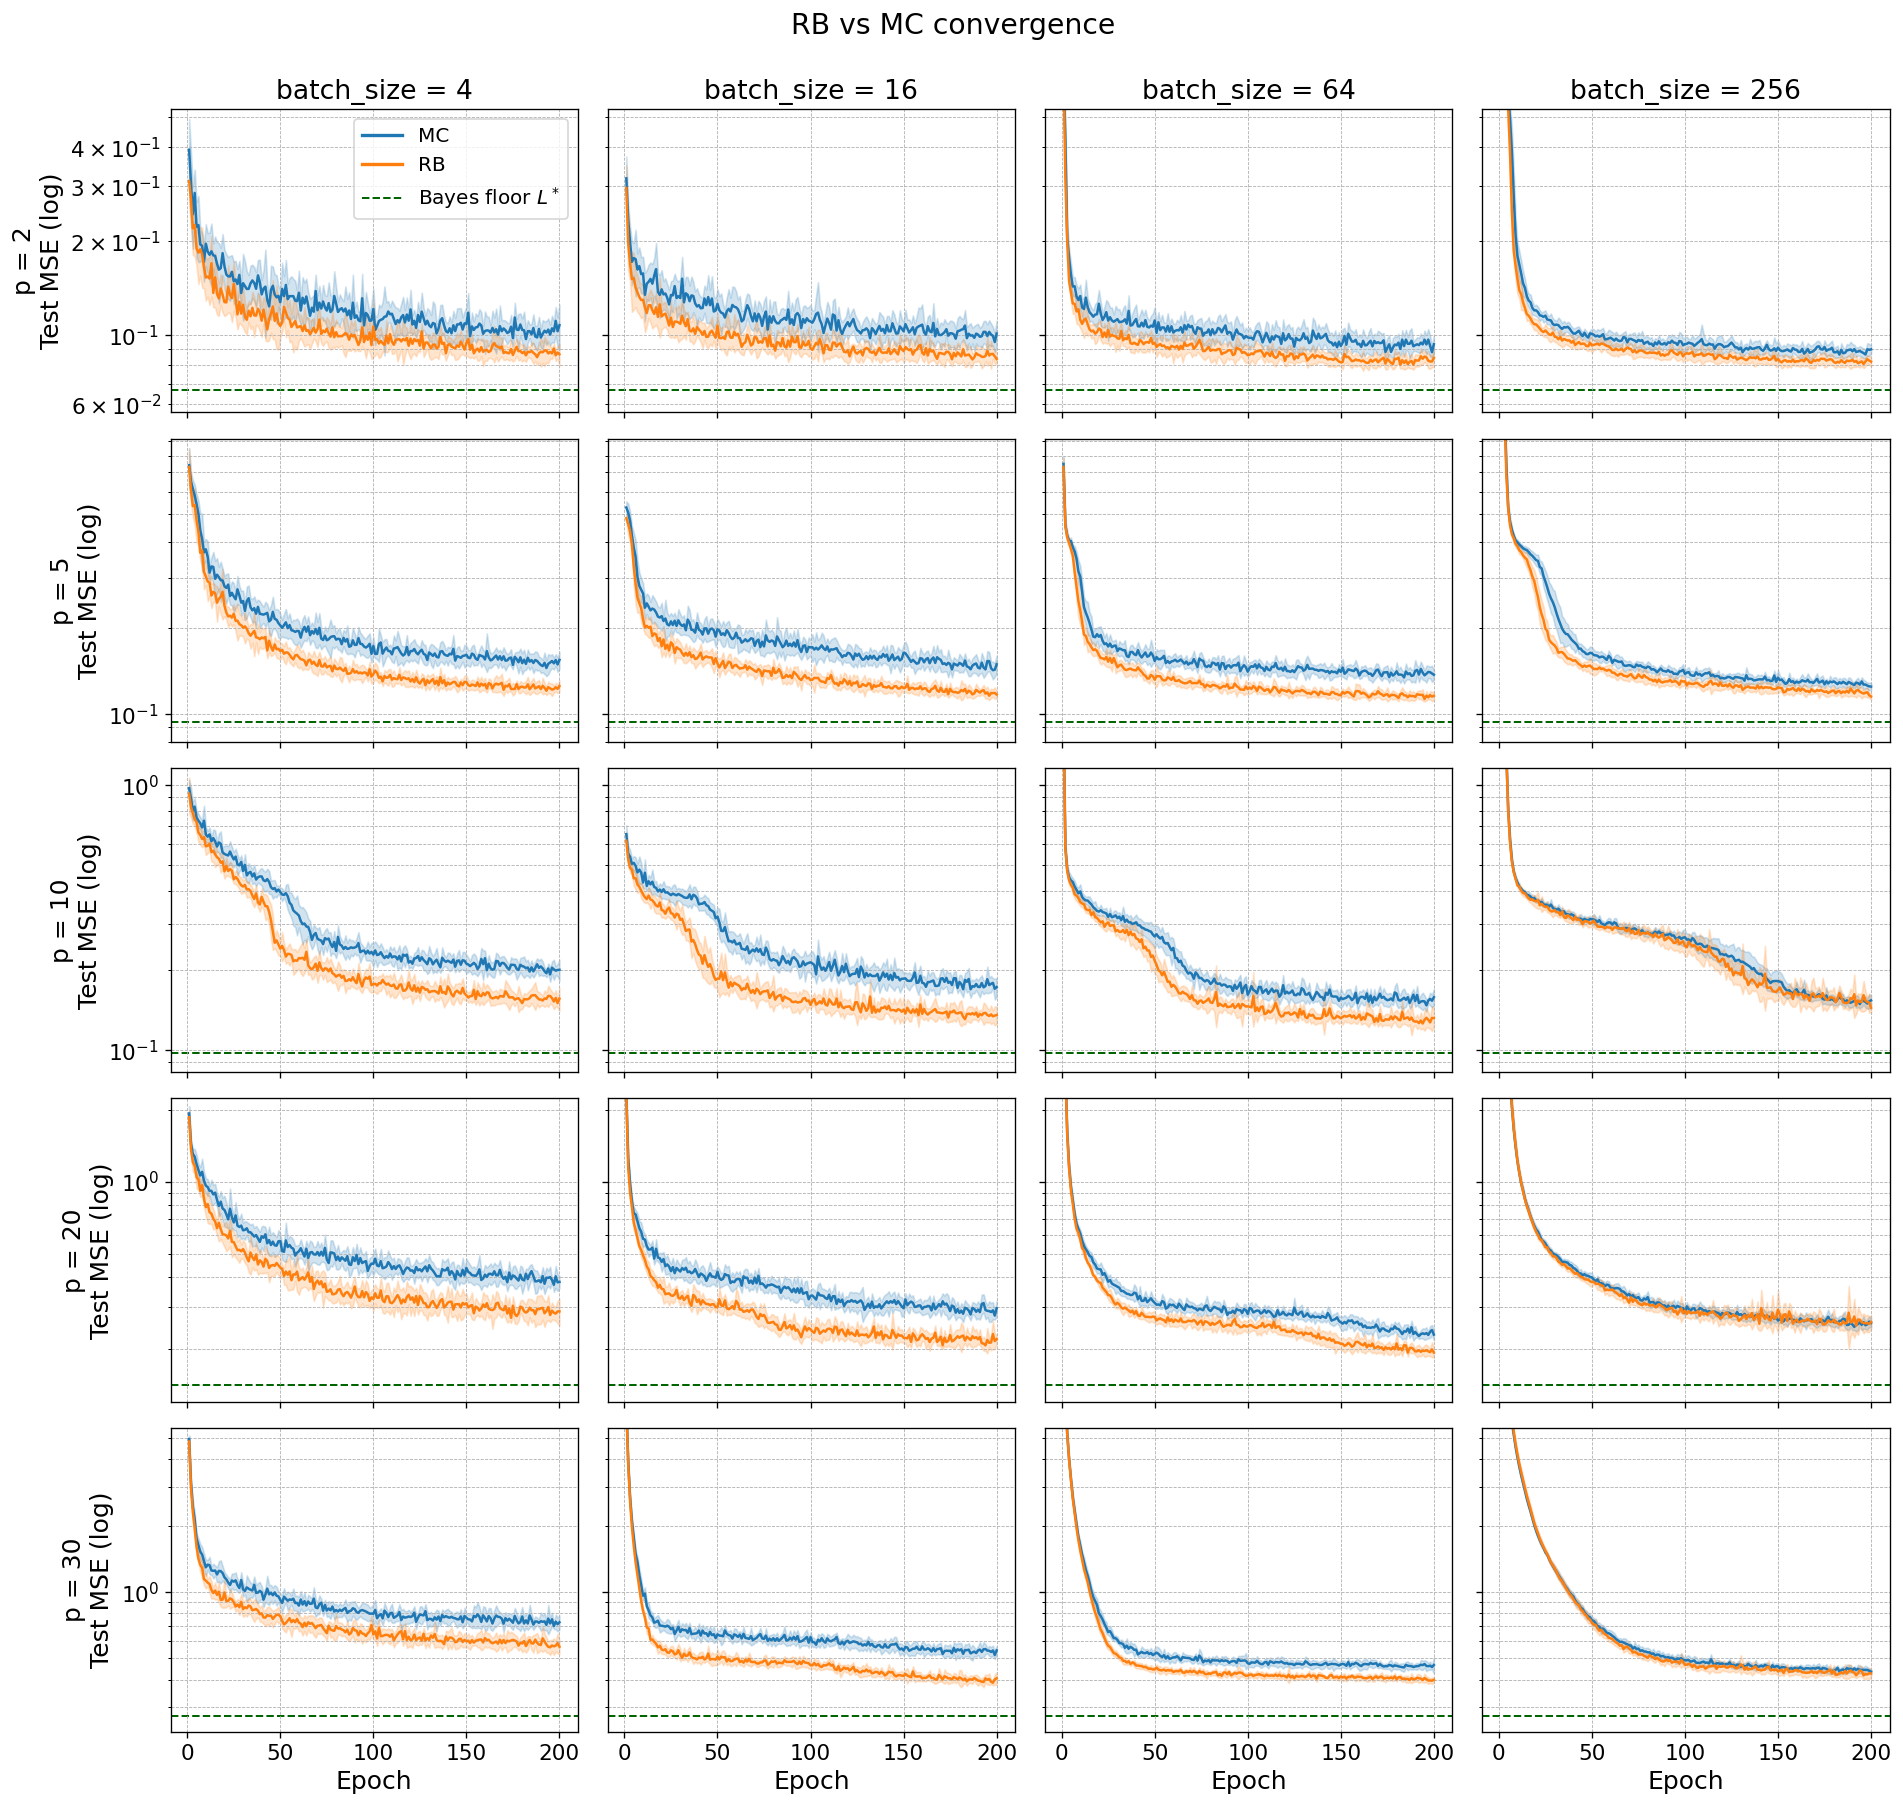
\includegraphics[width=\textwidth]{rb_tau_curves_X2}}
    {\fbox{\parbox[c][6cm][c]{\textwidth}{\centering\itshape
      Figure pending: second design-matrix curves grid
      (re-export \texttt{rb\_tau\_curves\_X2} via
      \texttt{replot\_curves\_floor.py}).}}}
  \caption{As Figure~\ref{fig:curves}, for the second design-matrix
  realisation $X^{(2)}$: training curves across parameter dimension $p$
  (rows) and batch size (columns); Monte Carlo (blue) and
  Rao-Blackwellised (orange), with the Bayes floor $L^{*}(p)$ dashed.}
  \label{fig:curves-X2}
\end{figure}

\begin{table}[htbp]
  \centering
  \small
  \caption{Second design matrix $X^{(2)}$: final test loss of the Monte
  Carlo (MC) and Rao-Blackwellised (RB) estimators, the Bayes floor
  $L^{*}$, and the raw and excess-over-floor ratios, for each $(p, B)$
  cell at $n = 50$.}
  \label{tab:main-grid-X2}
  \begin{tabular}{rr rrr rr}
    \toprule
    $p$ & $B$ & $\mathcal{L}_{\MC}$ & $\mathcal{L}_{\RB}$
        & $L^{*}$ & ratio & excess ratio \\
    \midrule
    2 & 4   & 0.1041 & 0.0882 & 0.0666 & 1.180 & 1.74 \\
    2 & 16  & 0.1001 & 0.0861 & 0.0666 & 1.162 & 1.72 \\
    2 & 64  & 0.0936 & 0.0838 & 0.0666 & 1.117 & 1.57 \\
    2 & 256 & 0.0889 & 0.0823 & 0.0666 & 1.080 & 1.42 \\
    \midrule
    5 & 4   & 0.1508 & 0.1234 & 0.0939 & 1.222 & 1.93 \\
    5 & 16  & 0.1471 & 0.1187 & 0.0939 & 1.240 & 2.15 \\
    5 & 64  & 0.1396 & 0.1160 & 0.0939 & 1.204 & 2.07 \\
    5 & 256 & 0.1271 & 0.1187 & 0.0939 & 1.070 & 1.34 \\
    \midrule
    10 & 4   & 0.2002 & 0.1561 & 0.0972 & 1.282 & 1.75 \\
    10 & 16  & 0.1762 & 0.1360 & 0.0972 & 1.295 & 2.04 \\
    10 & 64  & 0.1540 & 0.1294 & 0.0972 & 1.189 & 1.76 \\
    10 & 256 & 0.1524 & 0.1531 & 0.0972 & 0.995 & 0.99 \\
    \midrule
    20 & 4   & 0.3888 & 0.2864 & 0.1407 & 1.357 & 1.70 \\
    20 & 16  & 0.2912 & 0.2156 & 0.1407 & 1.351 & 2.01 \\
    20 & 64  & 0.2311 & 0.1953 & 0.1407 & 1.183 & 1.66 \\
    20 & 256 & 0.2538 & 0.2588 & 0.1407 & 0.981 & 0.96 \\
    \midrule
    30 & 4   & 0.7288 & 0.5779 & 0.2737 & 1.261 & 1.50 \\
    30 & 16  & 0.5409 & 0.3974 & 0.2737 & 1.361 & 2.16 \\
    30 & 64  & 0.4639 & 0.4018 & 0.2737 & 1.155 & 1.49 \\
    30 & 256 & 0.4435 & 0.4278 & 0.2737 & 1.037 & 1.10 \\
    \bottomrule
  \end{tabular}
\end{table}

% ----------------------------------------------------------------
\section{Reproduction}
\label{app:reproduction}

The experiment code is in \texttt{sweeps2/} of the accompanying
repository. The training curves of Figure~\ref{fig:curves} and the raw
per-cell trajectories are produced by
%
\begin{quote}
\texttt{python rb\_vs\_mc\_sweep\_tau.py}
\end{quote}
%
and the Bayes floors and the tables of this appendix by
\texttt{floors\_and\_tables.py}, which runs a vectorised Gibbs sampler
for the linear-regression posterior on the same held-out test sets. The
Bayes-floor line on Figure~\ref{fig:curves} is overlaid by
\texttt{replot\_curves\_floor.py}, and the samples-seen view of
Figure~\ref{fig:vs-samples} by \texttt{plot\_curves\_vs\_samples.py};
both reuse the saved \texttt{.npz} without retraining.


\bibliography{references}

\end{document}
